%%%%%%%%%%%%%%%%%%%%%%%%%%
% COM Dissertation Project Template
%%%%%%%%%%%%%%%%%%%%%%%%%%
% Based on template originally developed by
% Prof. Roger K. Moore
% University of Sheffield
% 22 March 2017
%%%%%%%%%%%%%%%%%%%%%%%%%%
% Updated 22 October 2025 (Mark Stevenson)
%%%%%%%%%%%%%%%%%%%%%%%%%%
%
% HOW THIS DOCUMENT IS BUILT (Overleaf: upload the whole dissertation/ folder as a zip, set
% main.tex as the main document, compiler pdfLaTeX; it compiles with the default settings)
%
%   Locally:  pdflatex main && bibtex main && pdflatex main && pdflatex main
%   Refresh the numbers and tables after any analysis change:  bash sync_generated.sh
%
% Every statistic in the text is a macro from generated/numbers.tex (for example \FullEmoSignObs{})
% so the prose cannot drift from the analysis. No result number is typed by hand.
% Boxes produced by \placeholderfigure are the images still to be added by hand; see
% FIGURES_TO_ADD.md for the list and the instructions.

\documentclass[11pt,oneside]{book}
\usepackage[margin=1.2in]{geometry}
\usepackage{setspace}
\usepackage[toc,page]{appendix}
\usepackage[none]{hyphenat} % turn hyphenation off by default (template setting)
\usepackage{graphicx}
\usepackage{amsmath,amssymb}
\usepackage{booktabs}
\usepackage{xcolor}
\usepackage{tikz}
\usetikzlibrary{arrows.meta,positioning,shapes.geometric,calc,fit}
\usepackage{microtype}
\usepackage{enumitem}
\usepackage{caption}
\usepackage{subcaption}
\usepackage{float}
\usepackage[most]{tcolorbox}
\usepackage{url}
\usepackage[hidelinks]{hyperref}

\emergencystretch 2em          % fewer overfull lines with hyphenation switched off
\captionsetup{font=small,labelfont=bf,width=0.92\textwidth}
\setlist{itemsep=2pt,topsep=3pt}

\graphicspath{{figures/}}
% numbers.tex — GENERATED by emoviz/export_tex.py. Do not edit; re-run the exporter.
% Every macro below is a number read from a result file under emoviz/outputs/.
% Macro                      Meaning
%   \nTotal                     records processed (incl. pre-tests)
%   \nPretest                   pre-festival developer test records, excluded
%   \nAnalysed                  records analysed
%   \nEmotional                 prompts whose GoEmotions top-1 family is not neutral
%   \nNonEmotional              prompts the text reader labels neutral
%   \nFaceAll                   face-classified records, all analysed
%   \nSceneAll                  scene-classified records, all analysed
%   \nFaceEmo                   face-classified within emotional
%   \nSceneEmo                  scene-classified within emotional
%   \nPositive                  positive-valence prompts (family joy)
%   \nNegative                  negative-valence prompts
%   \nDistinct                  distinct prompts (dedup_key groups)
%   \nRepeats                   records repeating an earlier prompt
%   \nHappy                     records whose prompt is exactly 'happy'
%   \nDistinctEmo               distinct prompts, emotional
%   \nDistinctNonEmo            distinct prompts, neutral-labelled
%   \nDistinctFace              distinct prompts, emotional, face-classified
%   \nDistinctScene             distinct prompts, emotional, scene-classified
%   \nGroups                    prompts drawn two or more times
%   \nGroupRecords              records inside those groups
%   \nPairGroups                groups that are pairs
%   \nullShuffles               random re-pairings per null
%   \nullSeed                   random seed of the analysis
%   \famPromptJoy               prompt-reader top-1 = joy, all analysed
%   \famPromptSadness           prompt-reader top-1 = sadness, all analysed
%   \famPromptAnger             prompt-reader top-1 = anger, all analysed
%   \famPromptFear              prompt-reader top-1 = fear, all analysed
%   \famPromptSurprise          prompt-reader top-1 = surprise, all analysed
%   \famPromptDisgust           prompt-reader top-1 = disgust, all analysed
%   \famPromptNeutral           prompt-reader top-1 = neutral, all analysed
%   \famImageJoy                image-reader top-1 = joy, all analysed
%   \famImageSadness            image-reader top-1 = sadness, all analysed
%   \famImageAnger              image-reader top-1 = anger, all analysed
%   \famImageFear               image-reader top-1 = fear, all analysed
%   \famImageSurprise           image-reader top-1 = surprise, all analysed
%   \famImageDisgust            image-reader top-1 = disgust, all analysed
%   \famImageNeutral            image-reader top-1 = neutral, all analysed
%   \FullEmoN                   Full block, ALL emotional: n
%   \FullEmoNSign               Full block, ALL emotional: valence-sign denominator
%   \FullEmoVaObs               Full ALL emotional va: observed
%   \FullEmoVaNull              Full ALL emotional va: null mean
%   \FullEmoVaSd                Full ALL emotional va: null sd (pp)
%   \FullEmoVaZ                 Full ALL emotional va: z (n/a = degenerate)
%   \FullEmoVaCi                Full ALL emotional va: clustered-bootstrap 95% CI
%   \FullEmoSignObs             Full ALL emotional vsign: observed
%   \FullEmoSignNull            Full ALL emotional vsign: null mean
%   \FullEmoSignSd              Full ALL emotional vsign: null sd (pp)
%   \FullEmoSignZ               Full ALL emotional vsign: z (n/a = degenerate)
%   \FullEmoSignCi              Full ALL emotional vsign: clustered-bootstrap 95% CI
%   \FullEmoFamObs              Full ALL emotional family: observed
%   \FullEmoFamNull             Full ALL emotional family: null mean
%   \FullEmoFamSd               Full ALL emotional family: null sd (pp)
%   \FullEmoFamZ                Full ALL emotional family: z (n/a = degenerate)
%   \FullEmoFamCi               Full ALL emotional family: clustered-bootstrap 95% CI
%   \FullEmoOvlpObs             Full ALL emotional overlap: observed
%   \FullEmoOvlpNull            Full ALL emotional overlap: null mean
%   \FullEmoOvlpSd              Full ALL emotional overlap: null sd (pp)
%   \FullEmoOvlpZ               Full ALL emotional overlap: z (n/a = degenerate)
%   \FullEmoOvlpCi              Full ALL emotional overlap: clustered-bootstrap 95% CI
%   \FullFaceN                  Full block, face images: n
%   \FullFaceNSign              Full block, face images: valence-sign denominator
%   \FullFaceVaObs              Full face images va: observed
%   \FullFaceVaNull             Full face images va: null mean
%   \FullFaceVaSd               Full face images va: null sd (pp)
%   \FullFaceVaZ                Full face images va: z (n/a = degenerate)
%   \FullFaceVaCi               Full face images va: clustered-bootstrap 95% CI
%   \FullFaceSignObs            Full face images vsign: observed
%   \FullFaceSignNull           Full face images vsign: null mean
%   \FullFaceSignSd             Full face images vsign: null sd (pp)
%   \FullFaceSignZ              Full face images vsign: z (n/a = degenerate)
%   \FullFaceSignCi             Full face images vsign: clustered-bootstrap 95% CI
%   \FullFaceFamObs             Full face images family: observed
%   \FullFaceFamNull            Full face images family: null mean
%   \FullFaceFamSd              Full face images family: null sd (pp)
%   \FullFaceFamZ               Full face images family: z (n/a = degenerate)
%   \FullFaceFamCi              Full face images family: clustered-bootstrap 95% CI
%   \FullFaceOvlpObs            Full face images overlap: observed
%   \FullFaceOvlpNull           Full face images overlap: null mean
%   \FullFaceOvlpSd             Full face images overlap: null sd (pp)
%   \FullFaceOvlpZ              Full face images overlap: z (n/a = degenerate)
%   \FullFaceOvlpCi             Full face images overlap: clustered-bootstrap 95% CI
%   \FullSceneN                 Full block, scene images: n
%   \FullSceneNSign             Full block, scene images: valence-sign denominator
%   \FullSceneVaObs             Full scene images va: observed
%   \FullSceneVaNull            Full scene images va: null mean
%   \FullSceneVaSd              Full scene images va: null sd (pp)
%   \FullSceneVaZ               Full scene images va: z (n/a = degenerate)
%   \FullSceneVaCi              Full scene images va: clustered-bootstrap 95% CI
%   \FullSceneSignObs           Full scene images vsign: observed
%   \FullSceneSignNull          Full scene images vsign: null mean
%   \FullSceneSignSd            Full scene images vsign: null sd (pp)
%   \FullSceneSignZ             Full scene images vsign: z (n/a = degenerate)
%   \FullSceneSignCi            Full scene images vsign: clustered-bootstrap 95% CI
%   \FullSceneFamObs            Full scene images family: observed
%   \FullSceneFamNull           Full scene images family: null mean
%   \FullSceneFamSd             Full scene images family: null sd (pp)
%   \FullSceneFamZ              Full scene images family: z (n/a = degenerate)
%   \FullSceneFamCi             Full scene images family: clustered-bootstrap 95% CI
%   \FullSceneOvlpObs           Full scene images overlap: observed
%   \FullSceneOvlpNull          Full scene images overlap: null mean
%   \FullSceneOvlpSd            Full scene images overlap: null sd (pp)
%   \FullSceneOvlpZ             Full scene images overlap: z (n/a = degenerate)
%   \FullSceneOvlpCi            Full scene images overlap: clustered-bootstrap 95% CI
%   \FullPosN                   Full block, positive prompts: n
%   \FullPosNSign               Full block, positive prompts: valence-sign denominator
%   \FullPosVaObs               Full positive prompts va: observed
%   \FullPosVaNull              Full positive prompts va: null mean
%   \FullPosVaSd                Full positive prompts va: null sd (pp)
%   \FullPosVaZ                 Full positive prompts va: z (n/a = degenerate)
%   \FullPosVaCi                Full positive prompts va: clustered-bootstrap 95% CI
%   \FullPosSignObs             Full positive prompts vsign: observed
%   \FullPosSignNull            Full positive prompts vsign: null mean
%   \FullPosSignSd              Full positive prompts vsign: null sd (pp)
%   \FullPosSignZ               Full positive prompts vsign: z (n/a = degenerate)
%   \FullPosSignCi              Full positive prompts vsign: clustered-bootstrap 95% CI
%   \FullPosFamObs              Full positive prompts family: observed
%   \FullPosFamNull             Full positive prompts family: null mean
%   \FullPosFamSd               Full positive prompts family: null sd (pp)
%   \FullPosFamZ                Full positive prompts family: z (n/a = degenerate)
%   \FullPosFamCi               Full positive prompts family: clustered-bootstrap 95% CI
%   \FullPosOvlpObs             Full positive prompts overlap: observed
%   \FullPosOvlpNull            Full positive prompts overlap: null mean
%   \FullPosOvlpSd              Full positive prompts overlap: null sd (pp)
%   \FullPosOvlpZ               Full positive prompts overlap: z (n/a = degenerate)
%   \FullPosOvlpCi              Full positive prompts overlap: clustered-bootstrap 95% CI
%   \FullNegN                   Full block, negative prompts: n
%   \FullNegNSign               Full block, negative prompts: valence-sign denominator
%   \FullNegVaObs               Full negative prompts va: observed
%   \FullNegVaNull              Full negative prompts va: null mean
%   \FullNegVaSd                Full negative prompts va: null sd (pp)
%   \FullNegVaZ                 Full negative prompts va: z (n/a = degenerate)
%   \FullNegVaCi                Full negative prompts va: clustered-bootstrap 95% CI
%   \FullNegSignObs             Full negative prompts vsign: observed
%   \FullNegSignNull            Full negative prompts vsign: null mean
%   \FullNegSignSd              Full negative prompts vsign: null sd (pp)
%   \FullNegSignZ               Full negative prompts vsign: z (n/a = degenerate)
%   \FullNegSignCi              Full negative prompts vsign: clustered-bootstrap 95% CI
%   \FullNegFamObs              Full negative prompts family: observed
%   \FullNegFamNull             Full negative prompts family: null mean
%   \FullNegFamSd               Full negative prompts family: null sd (pp)
%   \FullNegFamZ                Full negative prompts family: z (n/a = degenerate)
%   \FullNegFamCi               Full negative prompts family: clustered-bootstrap 95% CI
%   \FullNegOvlpObs             Full negative prompts overlap: observed
%   \FullNegOvlpNull            Full negative prompts overlap: null mean
%   \FullNegOvlpSd              Full negative prompts overlap: null sd (pp)
%   \FullNegOvlpZ               Full negative prompts overlap: z (n/a = degenerate)
%   \FullNegOvlpCi              Full negative prompts overlap: clustered-bootstrap 95% CI
%   \FullNeuN                   Full block, non-emotional: n
%   \FullNeuNSign               Full block, non-emotional: valence-sign denominator
%   \FullNeuVaObs               Full non-emotional va: observed
%   \FullNeuVaNull              Full non-emotional va: null mean
%   \FullNeuVaSd                Full non-emotional va: null sd (pp)
%   \FullNeuVaZ                 Full non-emotional va: z (n/a = degenerate)
%   \FullNeuVaCi                Full non-emotional va: clustered-bootstrap 95% CI
%   \FullNeuSignObs             Full non-emotional vsign: observed
%   \FullNeuSignNull            Full non-emotional vsign: null mean
%   \FullNeuSignSd              Full non-emotional vsign: null sd (pp)
%   \FullNeuSignZ               Full non-emotional vsign: z (n/a = degenerate)
%   \FullNeuSignCi              Full non-emotional vsign: clustered-bootstrap 95% CI
%   \FullNeuFamObs              Full non-emotional family: observed
%   \FullNeuFamNull             Full non-emotional family: null mean
%   \FullNeuFamSd               Full non-emotional family: null sd (pp)
%   \FullNeuFamZ                Full non-emotional family: z (n/a = degenerate)
%   \FullNeuFamCi               Full non-emotional family: clustered-bootstrap 95% CI
%   \FullNeuOvlpObs             Full non-emotional overlap: observed
%   \FullNeuOvlpNull            Full non-emotional overlap: null mean
%   \FullNeuOvlpSd              Full non-emotional overlap: null sd (pp)
%   \FullNeuOvlpZ               Full non-emotional overlap: z (n/a = degenerate)
%   \FullNeuOvlpCi              Full non-emotional overlap: clustered-bootstrap 95% CI
%   \DistEmoN                   Dist block, ALL emotional: n
%   \DistEmoNSign               Dist block, ALL emotional: valence-sign denominator
%   \DistEmoVaObs               Dist ALL emotional va: observed
%   \DistEmoVaNull              Dist ALL emotional va: null mean
%   \DistEmoVaSd                Dist ALL emotional va: null sd (pp)
%   \DistEmoVaZ                 Dist ALL emotional va: z (n/a = degenerate)
%   \DistEmoVaCi                Dist ALL emotional va: clustered-bootstrap 95% CI
%   \DistEmoSignObs             Dist ALL emotional vsign: observed
%   \DistEmoSignNull            Dist ALL emotional vsign: null mean
%   \DistEmoSignSd              Dist ALL emotional vsign: null sd (pp)
%   \DistEmoSignZ               Dist ALL emotional vsign: z (n/a = degenerate)
%   \DistEmoSignCi              Dist ALL emotional vsign: clustered-bootstrap 95% CI
%   \DistEmoFamObs              Dist ALL emotional family: observed
%   \DistEmoFamNull             Dist ALL emotional family: null mean
%   \DistEmoFamSd               Dist ALL emotional family: null sd (pp)
%   \DistEmoFamZ                Dist ALL emotional family: z (n/a = degenerate)
%   \DistEmoFamCi               Dist ALL emotional family: clustered-bootstrap 95% CI
%   \DistEmoOvlpObs             Dist ALL emotional overlap: observed
%   \DistEmoOvlpNull            Dist ALL emotional overlap: null mean
%   \DistEmoOvlpSd              Dist ALL emotional overlap: null sd (pp)
%   \DistEmoOvlpZ               Dist ALL emotional overlap: z (n/a = degenerate)
%   \DistEmoOvlpCi              Dist ALL emotional overlap: clustered-bootstrap 95% CI
%   \DistFaceN                  Dist block, face images: n
%   \DistFaceNSign              Dist block, face images: valence-sign denominator
%   \DistFaceVaObs              Dist face images va: observed
%   \DistFaceVaNull             Dist face images va: null mean
%   \DistFaceVaSd               Dist face images va: null sd (pp)
%   \DistFaceVaZ                Dist face images va: z (n/a = degenerate)
%   \DistFaceVaCi               Dist face images va: clustered-bootstrap 95% CI
%   \DistFaceSignObs            Dist face images vsign: observed
%   \DistFaceSignNull           Dist face images vsign: null mean
%   \DistFaceSignSd             Dist face images vsign: null sd (pp)
%   \DistFaceSignZ              Dist face images vsign: z (n/a = degenerate)
%   \DistFaceSignCi             Dist face images vsign: clustered-bootstrap 95% CI
%   \DistFaceFamObs             Dist face images family: observed
%   \DistFaceFamNull            Dist face images family: null mean
%   \DistFaceFamSd              Dist face images family: null sd (pp)
%   \DistFaceFamZ               Dist face images family: z (n/a = degenerate)
%   \DistFaceFamCi              Dist face images family: clustered-bootstrap 95% CI
%   \DistFaceOvlpObs            Dist face images overlap: observed
%   \DistFaceOvlpNull           Dist face images overlap: null mean
%   \DistFaceOvlpSd             Dist face images overlap: null sd (pp)
%   \DistFaceOvlpZ              Dist face images overlap: z (n/a = degenerate)
%   \DistFaceOvlpCi             Dist face images overlap: clustered-bootstrap 95% CI
%   \DistSceneN                 Dist block, scene images: n
%   \DistSceneNSign             Dist block, scene images: valence-sign denominator
%   \DistSceneVaObs             Dist scene images va: observed
%   \DistSceneVaNull            Dist scene images va: null mean
%   \DistSceneVaSd              Dist scene images va: null sd (pp)
%   \DistSceneVaZ               Dist scene images va: z (n/a = degenerate)
%   \DistSceneVaCi              Dist scene images va: clustered-bootstrap 95% CI
%   \DistSceneSignObs           Dist scene images vsign: observed
%   \DistSceneSignNull          Dist scene images vsign: null mean
%   \DistSceneSignSd            Dist scene images vsign: null sd (pp)
%   \DistSceneSignZ             Dist scene images vsign: z (n/a = degenerate)
%   \DistSceneSignCi            Dist scene images vsign: clustered-bootstrap 95% CI
%   \DistSceneFamObs            Dist scene images family: observed
%   \DistSceneFamNull           Dist scene images family: null mean
%   \DistSceneFamSd             Dist scene images family: null sd (pp)
%   \DistSceneFamZ              Dist scene images family: z (n/a = degenerate)
%   \DistSceneFamCi             Dist scene images family: clustered-bootstrap 95% CI
%   \DistSceneOvlpObs           Dist scene images overlap: observed
%   \DistSceneOvlpNull          Dist scene images overlap: null mean
%   \DistSceneOvlpSd            Dist scene images overlap: null sd (pp)
%   \DistSceneOvlpZ             Dist scene images overlap: z (n/a = degenerate)
%   \DistSceneOvlpCi            Dist scene images overlap: clustered-bootstrap 95% CI
%   \DistPosN                   Dist block, positive prompts: n
%   \DistPosNSign               Dist block, positive prompts: valence-sign denominator
%   \DistPosVaObs               Dist positive prompts va: observed
%   \DistPosVaNull              Dist positive prompts va: null mean
%   \DistPosVaSd                Dist positive prompts va: null sd (pp)
%   \DistPosVaZ                 Dist positive prompts va: z (n/a = degenerate)
%   \DistPosVaCi                Dist positive prompts va: clustered-bootstrap 95% CI
%   \DistPosSignObs             Dist positive prompts vsign: observed
%   \DistPosSignNull            Dist positive prompts vsign: null mean
%   \DistPosSignSd              Dist positive prompts vsign: null sd (pp)
%   \DistPosSignZ               Dist positive prompts vsign: z (n/a = degenerate)
%   \DistPosSignCi              Dist positive prompts vsign: clustered-bootstrap 95% CI
%   \DistPosFamObs              Dist positive prompts family: observed
%   \DistPosFamNull             Dist positive prompts family: null mean
%   \DistPosFamSd               Dist positive prompts family: null sd (pp)
%   \DistPosFamZ                Dist positive prompts family: z (n/a = degenerate)
%   \DistPosFamCi               Dist positive prompts family: clustered-bootstrap 95% CI
%   \DistPosOvlpObs             Dist positive prompts overlap: observed
%   \DistPosOvlpNull            Dist positive prompts overlap: null mean
%   \DistPosOvlpSd              Dist positive prompts overlap: null sd (pp)
%   \DistPosOvlpZ               Dist positive prompts overlap: z (n/a = degenerate)
%   \DistPosOvlpCi              Dist positive prompts overlap: clustered-bootstrap 95% CI
%   \DistNegN                   Dist block, negative prompts: n
%   \DistNegNSign               Dist block, negative prompts: valence-sign denominator
%   \DistNegVaObs               Dist negative prompts va: observed
%   \DistNegVaNull              Dist negative prompts va: null mean
%   \DistNegVaSd                Dist negative prompts va: null sd (pp)
%   \DistNegVaZ                 Dist negative prompts va: z (n/a = degenerate)
%   \DistNegVaCi                Dist negative prompts va: clustered-bootstrap 95% CI
%   \DistNegSignObs             Dist negative prompts vsign: observed
%   \DistNegSignNull            Dist negative prompts vsign: null mean
%   \DistNegSignSd              Dist negative prompts vsign: null sd (pp)
%   \DistNegSignZ               Dist negative prompts vsign: z (n/a = degenerate)
%   \DistNegSignCi              Dist negative prompts vsign: clustered-bootstrap 95% CI
%   \DistNegFamObs              Dist negative prompts family: observed
%   \DistNegFamNull             Dist negative prompts family: null mean
%   \DistNegFamSd               Dist negative prompts family: null sd (pp)
%   \DistNegFamZ                Dist negative prompts family: z (n/a = degenerate)
%   \DistNegFamCi               Dist negative prompts family: clustered-bootstrap 95% CI
%   \DistNegOvlpObs             Dist negative prompts overlap: observed
%   \DistNegOvlpNull            Dist negative prompts overlap: null mean
%   \DistNegOvlpSd              Dist negative prompts overlap: null sd (pp)
%   \DistNegOvlpZ               Dist negative prompts overlap: z (n/a = degenerate)
%   \DistNegOvlpCi              Dist negative prompts overlap: clustered-bootstrap 95% CI
%   \DistNeuN                   Dist block, non-emotional: n
%   \DistNeuNSign               Dist block, non-emotional: valence-sign denominator
%   \DistNeuVaObs               Dist non-emotional va: observed
%   \DistNeuVaNull              Dist non-emotional va: null mean
%   \DistNeuVaSd                Dist non-emotional va: null sd (pp)
%   \DistNeuVaZ                 Dist non-emotional va: z (n/a = degenerate)
%   \DistNeuVaCi                Dist non-emotional va: clustered-bootstrap 95% CI
%   \DistNeuSignObs             Dist non-emotional vsign: observed
%   \DistNeuSignNull            Dist non-emotional vsign: null mean
%   \DistNeuSignSd              Dist non-emotional vsign: null sd (pp)
%   \DistNeuSignZ               Dist non-emotional vsign: z (n/a = degenerate)
%   \DistNeuSignCi              Dist non-emotional vsign: clustered-bootstrap 95% CI
%   \DistNeuFamObs              Dist non-emotional family: observed
%   \DistNeuFamNull             Dist non-emotional family: null mean
%   \DistNeuFamSd               Dist non-emotional family: null sd (pp)
%   \DistNeuFamZ                Dist non-emotional family: z (n/a = degenerate)
%   \DistNeuFamCi               Dist non-emotional family: clustered-bootstrap 95% CI
%   \DistNeuOvlpObs             Dist non-emotional overlap: observed
%   \DistNeuOvlpNull            Dist non-emotional overlap: null mean
%   \DistNeuOvlpSd              Dist non-emotional overlap: null sd (pp)
%   \DistNeuOvlpZ               Dist non-emotional overlap: z (n/a = degenerate)
%   \DistNeuOvlpCi              Dist non-emotional overlap: clustered-bootstrap 95% CI
%   \DiffSignPp                 face minus scene, valence-sign agreement
%   \DiffSignCi                 its clustered-bootstrap 95% CI (pp)
%   \DiffSignP                  clustered permutation p (valence sign)
%   \DiffFamPp                  face minus scene, family agreement
%   \DiffFamCi                  its clustered-bootstrap 95% CI (pp)
%   \DiffFamP                   clustered permutation p (family)
%   \DiffDraws                  draws in the clustered bootstrap / permutation
%   \KappaEmo                   Cohen's kappa, family agreement, emotional
%   \KappaEmoCi                 its clustered-bootstrap 95% CI
%   \KappaEmoBand               Landis & Koch (1977) band
%   \KappaFace                  Cohen's kappa, family agreement, face
%   \KappaFaceCi                its clustered-bootstrap 95% CI
%   \KappaFaceBand              Landis & Koch (1977) band
%   \KappaScene                 Cohen's kappa, family agreement, scene
%   \KappaSceneCi               its clustered-bootstrap 95% CI
%   \KappaSceneBand             Landis & Koch (1977) band
%   \KappaAll                   Cohen's kappa, family agreement, all_analysed
%   \KappaAllCi                 its clustered-bootstrap 95% CI
%   \KappaAllBand               Landis & Koch (1977) band
%   \KappaDistEmo               Cohen's kappa, family agreement, distinct_emotional
%   \KappaDistEmoCi             its clustered-bootstrap 95% CI
%   \KappaDistEmoBand           Landis & Koch (1977) band
%   \KappaDistFace              Cohen's kappa, family agreement, distinct_face
%   \KappaDistFaceCi            its clustered-bootstrap 95% CI
%   \KappaDistFaceBand          Landis & Koch (1977) band
%   \KappaDistScene             Cohen's kappa, family agreement, distinct_scene
%   \KappaDistSceneCi           its clustered-bootstrap 95% CI
%   \KappaDistSceneBand         Landis & Koch (1977) band
%   \ConsFam                    mean within-group modal-family agreement
%   \ConsFamNull                its permutation-null mean
%   \ConsFamNullSd              its null sd
%   \ConsFamZ                   its z
%   \ConsFamP                   its permutation p
%   \ConsFamCi                  clustered-bootstrap 95% CI over groups (inference.py)
%   \ConsVal                    mean within-group modal-valence agreement
%   \ConsValNull                its null mean
%   \ConsValZ                   its z
%   \ConsValP                   its permutation p
%   \ConsFull                   groups where every drawing shares one family
%   \ConsFullPct                as a share of the groups
%   \ConsFullNull               its null mean (count)
%   \ConsFullZ                  its z
%   \ConsFullP                  its permutation p
%   \ConsDraws                  permutation draws
%   \ConsHappyN                 drawings of the prompt 'happy'
%   \ConsHappyJoy               'happy' drawings read as joy
%   \ConsHappyNeutral           'happy' drawings read as neutral
%   \ConsHappySurprise          'happy' drawings read as surprise
%   \ZSeedMin                   smallest emotional valence-sign z over seeds 1-5
%   \ZSeedMax                   largest emotional valence-sign z over seeds 1-5
%   \McN                        records both image readers cover
%   \McDeVa                     like-for-like describe_then_extract va (emotional)
%   \McDeVaNull                 its null mean
%   \McDeVaZ                    its z
%   \McDeSign                   like-for-like describe_then_extract vsign (emotional)
%   \McDeSignNull               its null mean
%   \McDeSignZ                  its z
%   \McDeFam                    like-for-like describe_then_extract family (emotional)
%   \McDeFamNull                its null mean
%   \McDeFamZ                   its z
%   \McDeOvlp                   like-for-like describe_then_extract overlap (emotional)
%   \McDeOvlpNull               its null mean
%   \McDeOvlpZ                  its z
%   \McDeFaceSign               like-for-like describe_then_extract face_images vsign
%   \McDeFaceSignZ              its z
%   \McDeFaceFam                like-for-like describe_then_extract face_images family
%   \McDeFaceFamZ               its z
%   \McDeSceneSign              like-for-like describe_then_extract scene_images vsign
%   \McDeSceneSignZ             its z
%   \McDeSceneFam               like-for-like describe_then_extract scene_images family
%   \McDeSceneFamZ              its z
%   \McClipVa                   like-for-like direct_clip va (emotional)
%   \McClipVaNull               its null mean
%   \McClipVaZ                  its z
%   \McClipSign                 like-for-like direct_clip vsign (emotional)
%   \McClipSignNull             its null mean
%   \McClipSignZ                its z
%   \McClipFam                  like-for-like direct_clip family (emotional)
%   \McClipFamNull              its null mean
%   \McClipFamZ                 its z
%   \McClipOvlp                 like-for-like direct_clip overlap (emotional)
%   \McClipOvlpNull             its null mean
%   \McClipOvlpZ                its z
%   \McClipFaceSign             like-for-like direct_clip face_images vsign
%   \McClipFaceSignZ            its z
%   \McClipFaceFam              like-for-like direct_clip face_images family
%   \McClipFaceFamZ             its z
%   \McClipSceneSign            like-for-like direct_clip scene_images vsign
%   \McClipSceneSignZ           its z
%   \McClipSceneFam             like-for-like direct_clip scene_images family
%   \McClipSceneFamZ            its z
%   \McDiffFamPp                describe minus CLIP, family agreement
%   \McDiffFamCi                its clustered-bootstrap 95% CI (pp)
%   \McMcNemarFamP              exact McNemar p, unclustered (optimistic)
%   \McClusterFamP              cluster sign-flip p (family)
%   \McFamB                     records only describe-then-extract agrees on (family)
%   \McFamC                     records only direct CLIP agrees on (family)
%   \McFamBoth                  records both agree on (family)
%   \McFamNeither               records neither agrees on (family)
%   \McDiffSignPp               describe minus CLIP, valence-sign agreement
%   \McDiffSignCi               its clustered-bootstrap 95% CI (pp)
%   \McMcNemarSignP             exact McNemar p, unclustered
%   \McClusterDraws             cluster sign-flip draws
%   \McReaderAgree              top-1 agreement between the two image readers
%   \McClipNeutral              emotional-prompt images direct CLIP reads as neutral
%   \McVOneN                    records in the v1 (NLI prompt side) comparison
%   \McVOneDeFam                v1 comparison describe_then_extract family
%   \McVOneDeOvlp               v1 comparison describe_then_extract overlap
%   \McVOneDeVa                 v1 comparison describe_then_extract va
%   \McVOneClipFam              v1 comparison direct_clip family
%   \McVOneClipOvlp             v1 comparison direct_clip overlap
%   \McVOneClipVa               v1 comparison direct_clip va
%   \CtrlN                      neutral-labelled prompts
%   \CtrlNameOnly               records reduced to '[name]' by redaction
%   \CtrlLexicon                affect words in the audit lexicon
%   \CtrlFlagged                neutral-labelled prompts containing an affect word
%   \CtrlFlaggedPct             as a share of the control
%   \CtrlRemoved                records removed for the cleaned control
%   \CtrlCleanN                 cleaned control size
%   \CtrlTopWords               ten most frequent affect words in the control
%   \CtrlVaObs                  full control VA observed
%   \CtrlVaNull                 full control VA null
%   \CtrlVaSd                   full control VA null sd (pp)
%   \CtrlVaZ                    full control VA z (record-level null)
%   \CtrlVaZClustered           full control VA z (clustered null)
%   \CtrlCleanVaObs             cleaned control VA observed
%   \CtrlCleanVaNull            cleaned control VA null
%   \CtrlCleanVaZ               cleaned control VA z (record-level)
%   \CtrlCleanVaZClustered      cleaned control VA z (clustered)
%   \CtrlFamObs                 full control family agreement (degenerate: equals its null)
%   \DescPeopleExpr             people>=1 and expression word
%   \DescPeopleNoExpr           people>=1, no expression word
%   \DescNoPeopleExpr           people=0 yet an expression word
%   \DescNoPeopleNoExpr         people=0, no expression word
%   \DescSceneN                 scene-classified records
%   \DescScenePeopleZero        of which people=0
%   \DescScenePeopleZeroExpr    of which people=0 with an expression word
%   \DescSceneSmile             people=0 answering smile/smiling/happy
%   \DescSceneSmilePct          as a share of the people=0 records
%   \DescBareStrictN            expression answers that name an affective state (strict)
%   \DescBareStrictPct          as a share of analysed records
%   \DescBareBroadN             expression answers that are a single facial-action or affect word (broad)
%   \DescCopyStrict             copy rate, strict: image top-1 equals the word's family
%   \DescCopyBroad              copy rate, broad
%   \DescCopyBroadPeopleZero    copy rate, broad, people=0
%   \DescCopyBroadPeople        copy rate, broad, people>=1
%   \DescSmileAll               smile/smiling/happy share, all analysed
%   \DescSmileAllN              count
%   \DescSmileFace              smile/smiling/happy share, face-classified
%   \DescSmileFaceN             count
%   \RecJoy                     per-family recall (row = prompt family joy)
%   \RecJoyCi                   its clustered-bootstrap 95% CI
%   \RecJoyN                    prompts in that family
%   \RecSadness                 per-family recall (row = prompt family sadness)
%   \RecSadnessCi               its clustered-bootstrap 95% CI
%   \RecSadnessN                prompts in that family
%   \RecAnger                   per-family recall (row = prompt family anger)
%   \RecAngerCi                 its clustered-bootstrap 95% CI
%   \RecAngerN                  prompts in that family
%   \RecFear                    per-family recall (row = prompt family fear)
%   \RecFearCi                  its clustered-bootstrap 95% CI
%   \RecFearN                   prompts in that family
%   \RecSurprise                per-family recall (row = prompt family surprise)
%   \RecSurpriseCi              its clustered-bootstrap 95% CI
%   \RecSurpriseN               prompts in that family
%   \RecDisgust                 per-family recall (row = prompt family disgust)
%   \RecDisgustCi               its clustered-bootstrap 95% CI
%   \RecDisgustN                prompts in that family
%   \TaxN                       high-confidence disagreements examined
%   \TaxDistinct                distinct prompts among them
%   \TaxA                       failure mode (a)
%   \TaxB                       failure mode (b)
%   \TaxC                       failure mode (c)
%   \TaxD                       failure mode (d)
%   \TaxE                       failure mode (e)
%   \TaxF                       failure mode (f)
%   \TaxDescriber               describer faults (a+b)
%   \TaxReader                  image-reader faults (c)
%   \TaxPrompt                  prompt-side faults (d+f)
%   \TaxGenerator               generator faults (e)
%   \TaxPeopleZero              records auto-tagged people=0
%   \HolmM                      non-degenerate z-scores tested
%   \HolmExcluded               degenerate z-scores excluded
%   \HolmSurvive                survive Holm at family-wise 0.05
%   \HolmFail                   do not survive
%   \HolmBonfZ                  Bonferroni-equivalent z for the smallest rank
%   \AblDropExpressionEmoSignObs ablation drop_expression, emotional, vsign: observed
%   \AblDropExpressionEmoSignNull ablation drop_expression, emotional, vsign: null mean
%   \AblDropExpressionEmoSignZ  ablation drop_expression, emotional, vsign: z
%   \AblDropExpressionEmoFamObs ablation drop_expression, emotional, family: observed
%   \AblDropExpressionEmoFamNull ablation drop_expression, emotional, family: null mean
%   \AblDropExpressionEmoFamZ   ablation drop_expression, emotional, family: z
%   \AblDropExpressionFaceSignObs ablation drop_expression, face, vsign: observed
%   \AblDropExpressionFaceSignNull ablation drop_expression, face, vsign: null mean
%   \AblDropExpressionFaceSignZ ablation drop_expression, face, vsign: z
%   \AblDropExpressionFaceFamObs ablation drop_expression, face, family: observed
%   \AblDropExpressionFaceFamNull ablation drop_expression, face, family: null mean
%   \AblDropExpressionFaceFamZ  ablation drop_expression, face, family: z
%   \AblDropExpressionSceneSignObs ablation drop_expression, scene, vsign: observed
%   \AblDropExpressionSceneSignNull ablation drop_expression, scene, vsign: null mean
%   \AblDropExpressionSceneSignZ ablation drop_expression, scene, vsign: z
%   \AblDropExpressionSceneFamObs ablation drop_expression, scene, family: observed
%   \AblDropExpressionSceneFamNull ablation drop_expression, scene, family: null mean
%   \AblDropExpressionSceneFamZ ablation drop_expression, scene, family: z
%   \AblDropActionEmoSignObs    ablation drop_action, emotional, vsign: observed
%   \AblDropActionEmoSignNull   ablation drop_action, emotional, vsign: null mean
%   \AblDropActionEmoSignZ      ablation drop_action, emotional, vsign: z
%   \AblDropActionEmoFamObs     ablation drop_action, emotional, family: observed
%   \AblDropActionEmoFamNull    ablation drop_action, emotional, family: null mean
%   \AblDropActionEmoFamZ       ablation drop_action, emotional, family: z
%   \AblDropActionFaceSignObs   ablation drop_action, face, vsign: observed
%   \AblDropActionFaceSignNull  ablation drop_action, face, vsign: null mean
%   \AblDropActionFaceSignZ     ablation drop_action, face, vsign: z
%   \AblDropActionFaceFamObs    ablation drop_action, face, family: observed
%   \AblDropActionFaceFamNull   ablation drop_action, face, family: null mean
%   \AblDropActionFaceFamZ      ablation drop_action, face, family: z
%   \AblDropActionSceneSignObs  ablation drop_action, scene, vsign: observed
%   \AblDropActionSceneSignNull ablation drop_action, scene, vsign: null mean
%   \AblDropActionSceneSignZ    ablation drop_action, scene, vsign: z
%   \AblDropActionSceneFamObs   ablation drop_action, scene, family: observed
%   \AblDropActionSceneFamNull  ablation drop_action, scene, family: null mean
%   \AblDropActionSceneFamZ     ablation drop_action, scene, family: z
%   \AblDropPostureEmoSignObs   ablation drop_posture, emotional, vsign: observed
%   \AblDropPostureEmoSignNull  ablation drop_posture, emotional, vsign: null mean
%   \AblDropPostureEmoSignZ     ablation drop_posture, emotional, vsign: z
%   \AblDropPostureEmoFamObs    ablation drop_posture, emotional, family: observed
%   \AblDropPostureEmoFamNull   ablation drop_posture, emotional, family: null mean
%   \AblDropPostureEmoFamZ      ablation drop_posture, emotional, family: z
%   \AblDropPostureFaceSignObs  ablation drop_posture, face, vsign: observed
%   \AblDropPostureFaceSignNull ablation drop_posture, face, vsign: null mean
%   \AblDropPostureFaceSignZ    ablation drop_posture, face, vsign: z
%   \AblDropPostureFaceFamObs   ablation drop_posture, face, family: observed
%   \AblDropPostureFaceFamNull  ablation drop_posture, face, family: null mean
%   \AblDropPostureFaceFamZ     ablation drop_posture, face, family: z
%   \AblDropPostureSceneSignObs ablation drop_posture, scene, vsign: observed
%   \AblDropPostureSceneSignNull ablation drop_posture, scene, vsign: null mean
%   \AblDropPostureSceneSignZ   ablation drop_posture, scene, vsign: z
%   \AblDropPostureSceneFamObs  ablation drop_posture, scene, family: observed
%   \AblDropPostureSceneFamNull ablation drop_posture, scene, family: null mean
%   \AblDropPostureSceneFamZ    ablation drop_posture, scene, family: z
%   \AblDropPeopleEmoSignObs    ablation drop_people, emotional, vsign: observed
%   \AblDropPeopleEmoSignNull   ablation drop_people, emotional, vsign: null mean
%   \AblDropPeopleEmoSignZ      ablation drop_people, emotional, vsign: z
%   \AblDropPeopleEmoFamObs     ablation drop_people, emotional, family: observed
%   \AblDropPeopleEmoFamNull    ablation drop_people, emotional, family: null mean
%   \AblDropPeopleEmoFamZ       ablation drop_people, emotional, family: z
%   \AblDropPeopleFaceSignObs   ablation drop_people, face, vsign: observed
%   \AblDropPeopleFaceSignNull  ablation drop_people, face, vsign: null mean
%   \AblDropPeopleFaceSignZ     ablation drop_people, face, vsign: z
%   \AblDropPeopleFaceFamObs    ablation drop_people, face, family: observed
%   \AblDropPeopleFaceFamNull   ablation drop_people, face, family: null mean
%   \AblDropPeopleFaceFamZ      ablation drop_people, face, family: z
%   \AblDropPeopleSceneSignObs  ablation drop_people, scene, vsign: observed
%   \AblDropPeopleSceneSignNull ablation drop_people, scene, vsign: null mean
%   \AblDropPeopleSceneSignZ    ablation drop_people, scene, vsign: z
%   \AblDropPeopleSceneFamObs   ablation drop_people, scene, family: observed
%   \AblDropPeopleSceneFamNull  ablation drop_people, scene, family: null mean
%   \AblDropPeopleSceneFamZ     ablation drop_people, scene, family: z
%   \AblDropSceneEmoSignObs     ablation drop_scene, emotional, vsign: observed
%   \AblDropSceneEmoSignNull    ablation drop_scene, emotional, vsign: null mean
%   \AblDropSceneEmoSignZ       ablation drop_scene, emotional, vsign: z
%   \AblDropSceneEmoFamObs      ablation drop_scene, emotional, family: observed
%   \AblDropSceneEmoFamNull     ablation drop_scene, emotional, family: null mean
%   \AblDropSceneEmoFamZ        ablation drop_scene, emotional, family: z
%   \AblDropSceneFaceSignObs    ablation drop_scene, face, vsign: observed
%   \AblDropSceneFaceSignNull   ablation drop_scene, face, vsign: null mean
%   \AblDropSceneFaceSignZ      ablation drop_scene, face, vsign: z
%   \AblDropSceneFaceFamObs     ablation drop_scene, face, family: observed
%   \AblDropSceneFaceFamNull    ablation drop_scene, face, family: null mean
%   \AblDropSceneFaceFamZ       ablation drop_scene, face, family: z
%   \AblDropSceneSceneSignObs   ablation drop_scene, scene, vsign: observed
%   \AblDropSceneSceneSignNull  ablation drop_scene, scene, vsign: null mean
%   \AblDropSceneSceneSignZ     ablation drop_scene, scene, vsign: z
%   \AblDropSceneSceneFamObs    ablation drop_scene, scene, family: observed
%   \AblDropSceneSceneFamNull   ablation drop_scene, scene, family: null mean
%   \AblDropSceneSceneFamZ      ablation drop_scene, scene, family: z
%   \AblFixedExpressionEmoSignObs ablation fixed_expression, emotional, vsign: observed
%   \AblFixedExpressionEmoSignNull ablation fixed_expression, emotional, vsign: null mean
%   \AblFixedExpressionEmoSignZ ablation fixed_expression, emotional, vsign: z
%   \AblFixedExpressionEmoFamObs ablation fixed_expression, emotional, family: observed
%   \AblFixedExpressionEmoFamNull ablation fixed_expression, emotional, family: null mean
%   \AblFixedExpressionEmoFamZ  ablation fixed_expression, emotional, family: z
%   \AblFixedExpressionFaceSignObs ablation fixed_expression, face, vsign: observed
%   \AblFixedExpressionFaceSignNull ablation fixed_expression, face, vsign: null mean
%   \AblFixedExpressionFaceSignZ ablation fixed_expression, face, vsign: z
%   \AblFixedExpressionFaceFamObs ablation fixed_expression, face, family: observed
%   \AblFixedExpressionFaceFamNull ablation fixed_expression, face, family: null mean
%   \AblFixedExpressionFaceFamZ ablation fixed_expression, face, family: z
%   \AblFixedExpressionSceneSignObs ablation fixed_expression, scene, vsign: observed
%   \AblFixedExpressionSceneSignNull ablation fixed_expression, scene, vsign: null mean
%   \AblFixedExpressionSceneSignZ ablation fixed_expression, scene, vsign: z
%   \AblFixedExpressionSceneFamObs ablation fixed_expression, scene, family: observed
%   \AblFixedExpressionSceneFamNull ablation fixed_expression, scene, family: null mean
%   \AblFixedExpressionSceneFamZ ablation fixed_expression, scene, family: z
%   \AblPeopleAwareEmoSignObs   ablation people_aware, emotional, vsign: observed
%   \AblPeopleAwareEmoSignNull  ablation people_aware, emotional, vsign: null mean
%   \AblPeopleAwareEmoSignZ     ablation people_aware, emotional, vsign: z
%   \AblPeopleAwareEmoFamObs    ablation people_aware, emotional, family: observed
%   \AblPeopleAwareEmoFamNull   ablation people_aware, emotional, family: null mean
%   \AblPeopleAwareEmoFamZ      ablation people_aware, emotional, family: z
%   \AblPeopleAwareFaceSignObs  ablation people_aware, face, vsign: observed
%   \AblPeopleAwareFaceSignNull ablation people_aware, face, vsign: null mean
%   \AblPeopleAwareFaceSignZ    ablation people_aware, face, vsign: z
%   \AblPeopleAwareFaceFamObs   ablation people_aware, face, family: observed
%   \AblPeopleAwareFaceFamNull  ablation people_aware, face, family: null mean
%   \AblPeopleAwareFaceFamZ     ablation people_aware, face, family: z
%   \AblPeopleAwareSceneSignObs ablation people_aware, scene, vsign: observed
%   \AblPeopleAwareSceneSignNull ablation people_aware, scene, vsign: null mean
%   \AblPeopleAwareSceneSignZ   ablation people_aware, scene, vsign: z
%   \AblPeopleAwareSceneFamObs  ablation people_aware, scene, family: observed
%   \AblPeopleAwareSceneFamNull ablation people_aware, scene, family: null mean
%   \AblPeopleAwareSceneFamZ    ablation people_aware, scene, family: z
%   \AblPeopleAwareNoExpressionEmoSignObs ablation people_aware_no_expression, emotional, vsign: observed
%   \AblPeopleAwareNoExpressionEmoSignNull ablation people_aware_no_expression, emotional, vsign: null mean
%   \AblPeopleAwareNoExpressionEmoSignZ ablation people_aware_no_expression, emotional, vsign: z
%   \AblPeopleAwareNoExpressionEmoFamObs ablation people_aware_no_expression, emotional, family: observed
%   \AblPeopleAwareNoExpressionEmoFamNull ablation people_aware_no_expression, emotional, family: null mean
%   \AblPeopleAwareNoExpressionEmoFamZ ablation people_aware_no_expression, emotional, family: z
%   \AblPeopleAwareNoExpressionFaceSignObs ablation people_aware_no_expression, face, vsign: observed
%   \AblPeopleAwareNoExpressionFaceSignNull ablation people_aware_no_expression, face, vsign: null mean
%   \AblPeopleAwareNoExpressionFaceSignZ ablation people_aware_no_expression, face, vsign: z
%   \AblPeopleAwareNoExpressionFaceFamObs ablation people_aware_no_expression, face, family: observed
%   \AblPeopleAwareNoExpressionFaceFamNull ablation people_aware_no_expression, face, family: null mean
%   \AblPeopleAwareNoExpressionFaceFamZ ablation people_aware_no_expression, face, family: z
%   \AblPeopleAwareNoExpressionSceneSignObs ablation people_aware_no_expression, scene, vsign: observed
%   \AblPeopleAwareNoExpressionSceneSignNull ablation people_aware_no_expression, scene, vsign: null mean
%   \AblPeopleAwareNoExpressionSceneSignZ ablation people_aware_no_expression, scene, vsign: z
%   \AblPeopleAwareNoExpressionSceneFamObs ablation people_aware_no_expression, scene, family: observed
%   \AblPeopleAwareNoExpressionSceneFamNull ablation people_aware_no_expression, scene, family: null mean
%   \AblPeopleAwareNoExpressionSceneFamZ ablation people_aware_no_expression, scene, family: z
%   \AblControlEmoSignObs       ablation control_full_template, emotional, vsign: observed
%   \AblControlEmoSignNull      ablation control_full_template, emotional, vsign: null mean
%   \AblControlEmoSignZ         ablation control_full_template, emotional, vsign: z
%   \AblControlEmoFamObs        ablation control_full_template, emotional, family: observed
%   \AblControlEmoFamNull       ablation control_full_template, emotional, family: null mean
%   \AblControlEmoFamZ          ablation control_full_template, emotional, family: z
%   \AblControlFaceSignObs      ablation control_full_template, face, vsign: observed
%   \AblControlFaceSignNull     ablation control_full_template, face, vsign: null mean
%   \AblControlFaceSignZ        ablation control_full_template, face, vsign: z
%   \AblControlFaceFamObs       ablation control_full_template, face, family: observed
%   \AblControlFaceFamNull      ablation control_full_template, face, family: null mean
%   \AblControlFaceFamZ         ablation control_full_template, face, family: z
%   \AblControlSceneSignObs     ablation control_full_template, scene, vsign: observed
%   \AblControlSceneSignNull    ablation control_full_template, scene, vsign: null mean
%   \AblControlSceneSignZ       ablation control_full_template, scene, vsign: z
%   \AblControlSceneFamObs      ablation control_full_template, scene, family: observed
%   \AblControlSceneFamNull     ablation control_full_template, scene, family: null mean
%   \AblControlSceneFamZ        ablation control_full_template, scene, family: z
%   \AblBaselineEmoSignObs      ablation baseline, emotional, vsign: observed
%   \AblBaselineEmoSignNull     ablation baseline, emotional, vsign: null mean
%   \AblBaselineEmoSignZ        ablation baseline, emotional, vsign: z
%   \AblBaselineEmoFamObs       ablation baseline, emotional, family: observed
%   \AblBaselineEmoFamNull      ablation baseline, emotional, family: null mean
%   \AblBaselineEmoFamZ         ablation baseline, emotional, family: z
%   \AblBaselineFaceSignObs     ablation baseline, face, vsign: observed
%   \AblBaselineFaceSignNull    ablation baseline, face, vsign: null mean
%   \AblBaselineFaceSignZ       ablation baseline, face, vsign: z
%   \AblBaselineFaceFamObs      ablation baseline, face, family: observed
%   \AblBaselineFaceFamNull     ablation baseline, face, family: null mean
%   \AblBaselineFaceFamZ        ablation baseline, face, family: z
%   \AblBaselineSceneSignObs    ablation baseline, scene, vsign: observed
%   \AblBaselineSceneSignNull   ablation baseline, scene, vsign: null mean
%   \AblBaselineSceneSignZ      ablation baseline, scene, vsign: z
%   \AblBaselineSceneFamObs     ablation baseline, scene, family: observed
%   \AblBaselineSceneFamNull    ablation baseline, scene, family: null mean
%   \AblBaselineSceneFamZ       ablation baseline, scene, family: z
%   \AblControlChanged          top-1 readings changed by the control re-run
%   \AblDropExpressionSurprise  drop_expression: records read as surprise
%   \AblDropExpressionNeutral   drop_expression: records read as neutral
%   \AblDropExpressionChanged   drop_expression: top-1 readings changed vs baseline
%   \AblationAvailable          ablation summary present
%   \HumanCheckAvailable        human check scored

\newcommand{\nTotal}{1,025}
\newcommand{\nPretest}{13}
\newcommand{\nAnalysed}{1,012}
\newcommand{\nEmotional}{607}
\newcommand{\nNonEmotional}{405}
\newcommand{\nFaceAll}{591}
\newcommand{\nSceneAll}{421}
\newcommand{\nFaceEmo}{402}
\newcommand{\nSceneEmo}{205}
\newcommand{\nPositive}{402}
\newcommand{\nNegative}{128}
\newcommand{\nDistinct}{763}
\newcommand{\nRepeats}{249}
\newcommand{\nHappy}{42}
\newcommand{\nDistinctEmo}{452}
\newcommand{\nDistinctNonEmo}{311}
\newcommand{\nDistinctFace}{319}
\newcommand{\nDistinctScene}{133}
\newcommand{\nGroups}{87}
\newcommand{\nGroupRecords}{336}
\newcommand{\nPairGroups}{43}
\newcommand{\nullShuffles}{300}
\newcommand{\nullSeed}{7}
\newcommand{\famPromptJoy}{402}
\newcommand{\famPromptSadness}{99}
\newcommand{\famPromptAnger}{12}
\newcommand{\famPromptFear}{16}
\newcommand{\famPromptSurprise}{77}
\newcommand{\famPromptDisgust}{1}
\newcommand{\famPromptNeutral}{405}
\newcommand{\famImageJoy}{461}
\newcommand{\famImageSadness}{141}
\newcommand{\famImageAnger}{89}
\newcommand{\famImageFear}{4}
\newcommand{\famImageSurprise}{108}
\newcommand{\famImageDisgust}{0}
\newcommand{\famImageNeutral}{209}
\newcommand{\FullEmoN}{607}
\newcommand{\FullEmoNSign}{530}
\newcommand{\FullEmoVaObs}{83.8\%}
\newcommand{\FullEmoVaNull}{77.3\%}
\newcommand{\FullEmoVaSd}{0.53\%}
\newcommand{\FullEmoVaZ}{+12.2}
\newcommand{\FullEmoVaCi}{[82.0, 85.5]}
\newcommand{\FullEmoSignObs}{64.0\%}
\newcommand{\FullEmoSignNull}{45.6\%}
\newcommand{\FullEmoSignSd}{1.65\%}
\newcommand{\FullEmoSignZ}{+11.1}
\newcommand{\FullEmoSignCi}{[58.6, 68.8]}
\newcommand{\FullEmoFamObs}{53.0\%}
\newcommand{\FullEmoFamNull}{38.8\%}
\newcommand{\FullEmoFamSd}{1.38\%}
\newcommand{\FullEmoFamZ}{+10.3}
\newcommand{\FullEmoFamCi}{[47.3, 58.7]}
\newcommand{\FullEmoOvlpObs}{50.6\%}
\newcommand{\FullEmoOvlpNull}{39.4\%}
\newcommand{\FullEmoOvlpSd}{0.96\%}
\newcommand{\FullEmoOvlpZ}{+11.6}
\newcommand{\FullEmoOvlpCi}{[46.5, 54.7]}
\newcommand{\FullFaceN}{402}
\newcommand{\FullFaceNSign}{360}
\newcommand{\FullFaceVaObs}{84.2\%}
\newcommand{\FullFaceVaNull}{76.4\%}
\newcommand{\FullFaceVaSd}{0.70\%}
\newcommand{\FullFaceVaZ}{+11.2}
\newcommand{\FullFaceVaCi}{[82.3, 86.1]}
\newcommand{\FullFaceSignObs}{73.9\%}
\newcommand{\FullFaceSignNull}{53.5\%}
\newcommand{\FullFaceSignSd}{1.97\%}
\newcommand{\FullFaceSignZ}{+10.4}
\newcommand{\FullFaceSignCi}{[68.3, 79.2]}
\newcommand{\FullFaceFamObs}{61.9\%}
\newcommand{\FullFaceFamNull}{45.8\%}
\newcommand{\FullFaceFamSd}{1.57\%}
\newcommand{\FullFaceFamZ}{+10.3}
\newcommand{\FullFaceFamCi}{[55.8, 68.0]}
\newcommand{\FullFaceOvlpObs}{53.4\%}
\newcommand{\FullFaceOvlpNull}{40.4\%}
\newcommand{\FullFaceOvlpSd}{1.12\%}
\newcommand{\FullFaceOvlpZ}{+11.6}
\newcommand{\FullFaceOvlpCi}{[49.2, 57.7]}
\newcommand{\FullSceneN}{205}
\newcommand{\FullSceneNSign}{170}
\newcommand{\FullSceneVaObs}{82.9\%}
\newcommand{\FullSceneVaNull}{79.1\%}
\newcommand{\FullSceneVaSd}{0.64\%}
\newcommand{\FullSceneVaZ}{+6.0}
\newcommand{\FullSceneVaCi}{[80.4, 85.2]}
\newcommand{\FullSceneSignObs}{42.9\%}
\newcommand{\FullSceneSignNull}{29.6\%}
\newcommand{\FullSceneSignSd}{2.30\%}
\newcommand{\FullSceneSignZ}{+5.8}
\newcommand{\FullSceneSignCi}{[33.1, 51.1]}
\newcommand{\FullSceneFamObs}{35.6\%}
\newcommand{\FullSceneFamNull}{26.2\%}
\newcommand{\FullSceneFamSd}{2.17\%}
\newcommand{\FullSceneFamZ}{+4.4}
\newcommand{\FullSceneFamCi}{[26.4, 44.1]}
\newcommand{\FullSceneOvlpObs}{44.9\%}
\newcommand{\FullSceneOvlpNull}{38.1\%}
\newcommand{\FullSceneOvlpSd}{1.39\%}
\newcommand{\FullSceneOvlpZ}{+4.9}
\newcommand{\FullSceneOvlpCi}{[38.7, 51.0]}
\newcommand{\FullPosN}{402}
\newcommand{\FullPosNSign}{402}
\newcommand{\FullPosVaObs}{86.6\%}
\newcommand{\FullPosVaNull}{85.9\%}
\newcommand{\FullPosVaSd}{0.19\%}
\newcommand{\FullPosVaZ}{+3.9}
\newcommand{\FullPosVaCi}{--}
\newcommand{\FullPosSignObs}{64.9\%}
\newcommand{\FullPosSignNull}{64.9\%}
\newcommand{\FullPosSignSd}{0.00\%}
\newcommand{\FullPosSignZ}{n/a}
\newcommand{\FullPosSignCi}{--}
\newcommand{\FullPosFamObs}{64.9\%}
\newcommand{\FullPosFamNull}{64.9\%}
\newcommand{\FullPosFamSd}{0.00\%}
\newcommand{\FullPosFamZ}{n/a}
\newcommand{\FullPosFamCi}{--}
\newcommand{\FullPosOvlpObs}{57.4\%}
\newcommand{\FullPosOvlpNull}{56.4\%}
\newcommand{\FullPosOvlpSd}{0.46\%}
\newcommand{\FullPosOvlpZ}{+2.3}
\newcommand{\FullPosOvlpCi}{--}
\newcommand{\FullNegN}{128}
\newcommand{\FullNegNSign}{128}
\newcommand{\FullNegVaObs}{75.9\%}
\newcommand{\FullNegVaNull}{74.5\%}
\newcommand{\FullNegVaSd}{0.66\%}
\newcommand{\FullNegVaZ}{+2.1}
\newcommand{\FullNegVaCi}{--}
\newcommand{\FullNegSignObs}{60.9\%}
\newcommand{\FullNegSignNull}{60.9\%}
\newcommand{\FullNegSignSd}{0.00\%}
\newcommand{\FullNegSignZ}{n/a}
\newcommand{\FullNegSignCi}{--}
\newcommand{\FullNegFamObs}{35.9\%}
\newcommand{\FullNegFamNull}{31.0\%}
\newcommand{\FullNegFamSd}{2.30\%}
\newcommand{\FullNegFamZ}{+2.1}
\newcommand{\FullNegFamCi}{--}
\newcommand{\FullNegOvlpObs}{35.4\%}
\newcommand{\FullNegOvlpNull}{30.3\%}
\newcommand{\FullNegOvlpSd}{1.68\%}
\newcommand{\FullNegOvlpZ}{+3.0}
\newcommand{\FullNegOvlpCi}{--}
\newcommand{\FullNeuN}{405}
\newcommand{\FullNeuNSign}{0}
\newcommand{\FullNeuVaObs}{76.6\%}
\newcommand{\FullNeuVaNull}{76.6\%}
\newcommand{\FullNeuVaSd}{0.16\%}
\newcommand{\FullNeuVaZ}{+0.3}
\newcommand{\FullNeuVaCi}{[75.6, 77.6]}
\newcommand{\FullNeuSignObs}{0.0\%}
\newcommand{\FullNeuSignNull}{0.0\%}
\newcommand{\FullNeuSignSd}{0.00\%}
\newcommand{\FullNeuSignZ}{n/a}
\newcommand{\FullNeuSignCi}{--}
\newcommand{\FullNeuFamObs}{28.6\%}
\newcommand{\FullNeuFamNull}{28.6\%}
\newcommand{\FullNeuFamSd}{0.00\%}
\newcommand{\FullNeuFamZ}{n/a}
\newcommand{\FullNeuFamCi}{--}
\newcommand{\FullNeuOvlpObs}{31.6\%}
\newcommand{\FullNeuOvlpNull}{31.6\%}
\newcommand{\FullNeuOvlpSd}{0.35\%}
\newcommand{\FullNeuOvlpZ}{+0.0}
\newcommand{\FullNeuOvlpCi}{--}
\newcommand{\DistEmoN}{452}
\newcommand{\DistEmoNSign}{394}
\newcommand{\DistEmoVaObs}{83.0\%}
\newcommand{\DistEmoVaNull}{76.5\%}
\newcommand{\DistEmoVaSd}{0.61\%}
\newcommand{\DistEmoVaZ}{+10.6}
\newcommand{\DistEmoVaCi}{[81.5, 84.4]}
\newcommand{\DistEmoSignObs}{62.2\%}
\newcommand{\DistEmoSignNull}{44.4\%}
\newcommand{\DistEmoSignSd}{1.80\%}
\newcommand{\DistEmoSignZ}{+9.9}
\newcommand{\DistEmoSignCi}{[57.2, 67.0]}
\newcommand{\DistEmoFamObs}{51.3\%}
\newcommand{\DistEmoFamNull}{37.2\%}
\newcommand{\DistEmoFamSd}{1.51\%}
\newcommand{\DistEmoFamZ}{+9.3}
\newcommand{\DistEmoFamCi}{[46.7, 56.0]}
\newcommand{\DistEmoOvlpObs}{48.9\%}
\newcommand{\DistEmoOvlpNull}{37.7\%}
\newcommand{\DistEmoOvlpSd}{1.03\%}
\newcommand{\DistEmoOvlpZ}{+10.8}
\newcommand{\DistEmoOvlpCi}{[45.9, 51.9]}
\newcommand{\DistFaceN}{319}
\newcommand{\DistFaceNSign}{284}
\newcommand{\DistFaceVaObs}{83.5\%}
\newcommand{\DistFaceVaNull}{75.5\%}
\newcommand{\DistFaceVaSd}{0.82\%}
\newcommand{\DistFaceVaZ}{+9.7}
\newcommand{\DistFaceVaCi}{[81.7, 85.2]}
\newcommand{\DistFaceSignObs}{71.8\%}
\newcommand{\DistFaceSignNull}{51.0\%}
\newcommand{\DistFaceSignSd}{2.46\%}
\newcommand{\DistFaceSignZ}{+8.4}
\newcommand{\DistFaceSignCi}{[66.4, 77.0]}
\newcommand{\DistFaceFamObs}{59.9\%}
\newcommand{\DistFaceFamNull}{43.0\%}
\newcommand{\DistFaceFamSd}{2.07\%}
\newcommand{\DistFaceFamZ}{+8.1}
\newcommand{\DistFaceFamCi}{[54.2, 65.2]}
\newcommand{\DistFaceOvlpObs}{51.8\%}
\newcommand{\DistFaceOvlpNull}{38.4\%}
\newcommand{\DistFaceOvlpSd}{1.38\%}
\newcommand{\DistFaceOvlpZ}{+9.7}
\newcommand{\DistFaceOvlpCi}{[48.1, 55.4]}
\newcommand{\DistSceneN}{133}
\newcommand{\DistSceneNSign}{110}
\newcommand{\DistSceneVaObs}{81.8\%}
\newcommand{\DistSceneVaNull}{78.9\%}
\newcommand{\DistSceneVaSd}{0.80\%}
\newcommand{\DistSceneVaZ}{+3.6}
\newcommand{\DistSceneVaCi}{[79.5, 83.8]}
\newcommand{\DistSceneSignObs}{37.3\%}
\newcommand{\DistSceneSignNull}{27.1\%}
\newcommand{\DistSceneSignSd}{2.92\%}
\newcommand{\DistSceneSignZ}{+3.5}
\newcommand{\DistSceneSignCi}{[28.1, 46.2]}
\newcommand{\DistSceneFamObs}{30.8\%}
\newcommand{\DistSceneFamNull}{24.1\%}
\newcommand{\DistSceneFamSd}{2.62\%}
\newcommand{\DistSceneFamZ}{+2.6}
\newcommand{\DistSceneFamCi}{[23.3, 38.4]}
\newcommand{\DistSceneOvlpObs}{41.7\%}
\newcommand{\DistSceneOvlpNull}{36.7\%}
\newcommand{\DistSceneOvlpSd}{1.63\%}
\newcommand{\DistSceneOvlpZ}{+3.1}
\newcommand{\DistSceneOvlpCi}{[36.9, 46.5]}
\newcommand{\DistPosN}{293}
\newcommand{\DistPosNSign}{293}
\newcommand{\DistPosVaObs}{85.5\%}
\newcommand{\DistPosVaNull}{84.8\%}
\newcommand{\DistPosVaSd}{0.22\%}
\newcommand{\DistPosVaZ}{+3.3}
\newcommand{\DistPosVaCi}{--}
\newcommand{\DistPosSignObs}{62.1\%}
\newcommand{\DistPosSignNull}{62.1\%}
\newcommand{\DistPosSignSd}{0.00\%}
\newcommand{\DistPosSignZ}{n/a}
\newcommand{\DistPosSignCi}{--}
\newcommand{\DistPosFamObs}{62.1\%}
\newcommand{\DistPosFamNull}{62.1\%}
\newcommand{\DistPosFamSd}{0.00\%}
\newcommand{\DistPosFamZ}{n/a}
\newcommand{\DistPosFamCi}{--}
\newcommand{\DistPosOvlpObs}{54.6\%}
\newcommand{\DistPosOvlpNull}{53.6\%}
\newcommand{\DistPosOvlpSd}{0.53\%}
\newcommand{\DistPosOvlpZ}{+1.9}
\newcommand{\DistPosOvlpCi}{--}
\newcommand{\DistNegN}{101}
\newcommand{\DistNegNSign}{101}
\newcommand{\DistNegVaObs}{76.2\%}
\newcommand{\DistNegVaNull}{74.8\%}
\newcommand{\DistNegVaSd}{0.85\%}
\newcommand{\DistNegVaZ}{+1.6}
\newcommand{\DistNegVaCi}{--}
\newcommand{\DistNegSignObs}{62.4\%}
\newcommand{\DistNegSignNull}{62.4\%}
\newcommand{\DistNegSignSd}{0.00\%}
\newcommand{\DistNegSignZ}{n/a}
\newcommand{\DistNegSignCi}{--}
\newcommand{\DistNegFamObs}{38.6\%}
\newcommand{\DistNegFamNull}{32.9\%}
\newcommand{\DistNegFamSd}{2.72\%}
\newcommand{\DistNegFamZ}{+2.1}
\newcommand{\DistNegFamCi}{--}
\newcommand{\DistNegOvlpObs}{36.7\%}
\newcommand{\DistNegOvlpNull}{31.0\%}
\newcommand{\DistNegOvlpSd}{2.11\%}
\newcommand{\DistNegOvlpZ}{+2.7}
\newcommand{\DistNegOvlpCi}{--}
\newcommand{\DistNeuN}{311}
\newcommand{\DistNeuNSign}{0}
\newcommand{\DistNeuVaObs}{76.6\%}
\newcommand{\DistNeuVaNull}{76.4\%}
\newcommand{\DistNeuVaSd}{0.18\%}
\newcommand{\DistNeuVaZ}{+1.1}
\newcommand{\DistNeuVaCi}{--}
\newcommand{\DistNeuSignObs}{0.0\%}
\newcommand{\DistNeuSignNull}{0.0\%}
\newcommand{\DistNeuSignSd}{0.00\%}
\newcommand{\DistNeuSignZ}{n/a}
\newcommand{\DistNeuSignCi}{--}
\newcommand{\DistNeuFamObs}{27.7\%}
\newcommand{\DistNeuFamNull}{27.7\%}
\newcommand{\DistNeuFamSd}{0.00\%}
\newcommand{\DistNeuFamZ}{n/a}
\newcommand{\DistNeuFamCi}{--}
\newcommand{\DistNeuOvlpObs}{31.4\%}
\newcommand{\DistNeuOvlpNull}{31.1\%}
\newcommand{\DistNeuOvlpSd}{0.37\%}
\newcommand{\DistNeuOvlpZ}{+0.8}
\newcommand{\DistNeuOvlpCi}{--}
\newcommand{\DiffSignPp}{+30.9~pp}
\newcommand{\DiffSignCi}{[+22.6, +40.6]}
\newcommand{\DiffSignP}{0.0001}
\newcommand{\DiffFamPp}{+26.3~pp}
\newcommand{\DiffFamCi}{[+18.4, +35.3]}
\newcommand{\DiffFamP}{0.0001}
\newcommand{\DiffDraws}{10,000}
\newcommand{\KappaEmo}{0.23}
\newcommand{\KappaEmoCi}{[0.18, 0.29]}
\newcommand{\KappaEmoBand}{fair}
\newcommand{\KappaFace}{0.30}
\newcommand{\KappaFaceCi}{[0.23, 0.37]}
\newcommand{\KappaFaceBand}{fair}
\newcommand{\KappaScene}{0.13}
\newcommand{\KappaSceneCi}{[0.06, 0.19]}
\newcommand{\KappaSceneBand}{slight}
\newcommand{\KappaAll}{0.21}
\newcommand{\KappaAllCi}{[0.16, 0.25]}
\newcommand{\KappaAllBand}{fair}
\newcommand{\KappaDistEmo}{0.23}
\newcommand{\KappaDistEmoCi}{[0.17, 0.29]}
\newcommand{\KappaDistEmoBand}{fair}
\newcommand{\KappaDistFace}{0.29}
\newcommand{\KappaDistFaceCi}{[0.21, 0.37]}
\newcommand{\KappaDistFaceBand}{fair}
\newcommand{\KappaDistScene}{0.09}
\newcommand{\KappaDistSceneCi}{[0.01, 0.17]}
\newcommand{\KappaDistSceneBand}{slight}
\newcommand{\ConsFam}{68.8\%}
\newcommand{\ConsFamNull}{59.4\%}
\newcommand{\ConsFamNullSd}{2.1\%}
\newcommand{\ConsFamZ}{+4.5}
\newcommand{\ConsFamP}{$1.0\times10^{-4}$}
\newcommand{\ConsFamCi}{[63.8, 73.9]}
\newcommand{\ConsVal}{74.5\%}
\newcommand{\ConsValNull}{63.7\%}
\newcommand{\ConsValZ}{+5.0}
\newcommand{\ConsValP}{$1.0\times10^{-4}$}
\newcommand{\ConsFull}{28}
\newcommand{\ConsFullPct}{32.2\%}
\newcommand{\ConsFullNull}{14.5}
\newcommand{\ConsFullZ}{+4.2}
\newcommand{\ConsFullP}{$2.0\times10^{-4}$}
\newcommand{\ConsDraws}{10,000}
\newcommand{\ConsHappyN}{42}
\newcommand{\ConsHappyJoy}{34}
\newcommand{\ConsHappyNeutral}{7}
\newcommand{\ConsHappySurprise}{1}
\newcommand{\ZSeedMin}{+11.2}
\newcommand{\ZSeedMax}{+12.2}
\newcommand{\McN}{607}
\newcommand{\McDeVa}{83.8\%}
\newcommand{\McDeVaNull}{77.3\%}
\newcommand{\McDeVaZ}{+12.2}
\newcommand{\McDeSign}{64.0\%}
\newcommand{\McDeSignNull}{45.6\%}
\newcommand{\McDeSignZ}{+11.1}
\newcommand{\McDeFam}{53.0\%}
\newcommand{\McDeFamNull}{38.8\%}
\newcommand{\McDeFamZ}{+10.3}
\newcommand{\McDeOvlp}{50.6\%}
\newcommand{\McDeOvlpNull}{39.4\%}
\newcommand{\McDeOvlpZ}{+11.6}
\newcommand{\McDeFaceSign}{73.9\%}
\newcommand{\McDeFaceSignZ}{+10.4}
\newcommand{\McDeFaceFam}{61.9\%}
\newcommand{\McDeFaceFamZ}{+10.3}
\newcommand{\McDeSceneSign}{42.9\%}
\newcommand{\McDeSceneSignZ}{+5.8}
\newcommand{\McDeSceneFam}{35.6\%}
\newcommand{\McDeSceneFamZ}{+4.4}
\newcommand{\McClipVa}{73.3\%}
\newcommand{\McClipVaNull}{70.1\%}
\newcommand{\McClipVaZ}{+10.2}
\newcommand{\McClipSign}{31.1\%}
\newcommand{\McClipSignNull}{18.6\%}
\newcommand{\McClipSignZ}{+9.9}
\newcommand{\McClipFam}{22.4\%}
\newcommand{\McClipFamNull}{12.2\%}
\newcommand{\McClipFamZ}{+11.1}
\newcommand{\McClipOvlp}{26.4\%}
\newcommand{\McClipOvlpNull}{20.2\%}
\newcommand{\McClipOvlpZ}{+11.2}
\newcommand{\McClipFaceSign}{36.4\%}
\newcommand{\McClipFaceSignZ}{+7.9}
\newcommand{\McClipFaceFam}{27.4\%}
\newcommand{\McClipFaceFamZ}{+9.4}
\newcommand{\McClipSceneSign}{20.0\%}
\newcommand{\McClipSceneSignZ}{+5.4}
\newcommand{\McClipSceneFam}{12.7\%}
\newcommand{\McClipSceneFamZ}{+4.1}
\newcommand{\McDiffFamPp}{+30.6~pp}
\newcommand{\McDiffFamCi}{[+25.5, +35.6]}
\newcommand{\McMcNemarFamP}{$3.4\times10^{-35}$}
\newcommand{\McClusterFamP}{$<$0.001}
\newcommand{\McFamB}{218}
\newcommand{\McFamC}{32}
\newcommand{\McFamBoth}{104}
\newcommand{\McFamNeither}{253}
\newcommand{\McDiffSignPp}{+32.8~pp}
\newcommand{\McDiffSignCi}{[+27.4, +38.2]}
\newcommand{\McMcNemarSignP}{$5.5\times10^{-33}$}
\newcommand{\McClusterDraws}{20,000}
\newcommand{\McReaderAgree}{32.1\%}
\newcommand{\McClipNeutral}{283}
\newcommand{\McVOneN}{608}
\newcommand{\McVOneDeFam}{49.3\%}
\newcommand{\McVOneDeOvlp}{48.6\%}
\newcommand{\McVOneDeVa}{83.7\%}
\newcommand{\McVOneClipFam}{25.3\%}
\newcommand{\McVOneClipOvlp}{22.8\%}
\newcommand{\McVOneClipVa}{74.2\%}
\newcommand{\CtrlN}{405}
\newcommand{\CtrlNameOnly}{2}
\newcommand{\CtrlLexicon}{66}
\newcommand{\CtrlFlagged}{68}
\newcommand{\CtrlFlaggedPct}{16.8\%}
\newcommand{\CtrlRemoved}{70}
\newcommand{\CtrlCleanN}{335}
\newcommand{\CtrlTopWords}{calm (10), content (8), tired (7), stress (6), relaxed (6), inspired (4), sleepy (4), interested (3), anticipation (3), nostalgic (3)}
\newcommand{\CtrlVaObs}{76.6\%}
\newcommand{\CtrlVaNull}{76.5\%}
\newcommand{\CtrlVaSd}{0.15\%}
\newcommand{\CtrlVaZ}{+0.5}
\newcommand{\CtrlVaZClustered}{-0.1}
\newcommand{\CtrlCleanVaObs}{76.6\%}
\newcommand{\CtrlCleanVaNull}{76.6\%}
\newcommand{\CtrlCleanVaZ}{+0.0}
\newcommand{\CtrlCleanVaZClustered}{-0.6}
\newcommand{\CtrlFamObs}{28.6\%}
\newcommand{\DescPeopleExpr}{591}
\newcommand{\DescPeopleNoExpr}{7}
\newcommand{\DescNoPeopleExpr}{406}
\newcommand{\DescNoPeopleNoExpr}{8}
\newcommand{\DescSceneN}{421}
\newcommand{\DescScenePeopleZero}{414}
\newcommand{\DescScenePeopleZeroExpr}{406}
\newcommand{\DescSceneSmile}{332}
\newcommand{\DescSceneSmilePct}{80.2\%}
\newcommand{\DescBareStrictN}{418}
\newcommand{\DescBareStrictPct}{41.3\%}
\newcommand{\DescBareBroadN}{997}
\newcommand{\DescCopyStrict}{99.8\%}
\newcommand{\DescCopyBroad}{68.6\%}
\newcommand{\DescCopyBroadPeopleZero}{48.8\%}
\newcommand{\DescCopyBroadPeople}{82.2\%}
\newcommand{\DescSmileAll}{66.1\%}
\newcommand{\DescSmileAllN}{669}
\newcommand{\DescSmileFace}{57.0\%}
\newcommand{\DescSmileFaceN}{337}
\newcommand{\RecJoy}{64.9\%}
\newcommand{\RecJoyCi}{[58.7, 70.3]}
\newcommand{\RecJoyN}{402}
\newcommand{\RecSadness}{40.4\%}
\newcommand{\RecSadnessCi}{[30.9, 51.2]}
\newcommand{\RecSadnessN}{99}
\newcommand{\RecAnger}{50.0\%}
\newcommand{\RecAngerCi}{[22.2, 77.8]}
\newcommand{\RecAngerN}{12}
\newcommand{\RecFear}{0.0\%}
\newcommand{\RecFearCi}{[0.0, 0.0]}
\newcommand{\RecFearN}{16}
\newcommand{\RecSurprise}{19.5\%}
\newcommand{\RecSurpriseCi}{[11.4, 28.1]}
\newcommand{\RecSurpriseN}{77}
\newcommand{\RecDisgust}{0.0\%}
\newcommand{\RecDisgustCi}{[0.0, 0.0]}
\newcommand{\RecDisgustN}{1}
\newcommand{\TaxN}{38}
\newcommand{\TaxDistinct}{37}
\newcommand{\TaxA}{9}
\newcommand{\TaxB}{10}
\newcommand{\TaxC}{5}
\newcommand{\TaxD}{11}
\newcommand{\TaxE}{2}
\newcommand{\TaxF}{1}
\newcommand{\TaxDescriber}{19}
\newcommand{\TaxReader}{5}
\newcommand{\TaxPrompt}{12}
\newcommand{\TaxGenerator}{2}
\newcommand{\TaxPeopleZero}{13}
\newcommand{\HolmM}{36}
\newcommand{\HolmExcluded}{12}
\newcommand{\HolmSurvive}{26}
\newcommand{\HolmFail}{10}
\newcommand{\HolmBonfZ}{3.2}
\newcommand{\AblDropExpressionEmoSignObs}{15.3\%}
\newcommand{\AblDropExpressionEmoSignNull}{11.4\%}
\newcommand{\AblDropExpressionEmoSignZ}{+5.1}
\newcommand{\AblDropExpressionEmoFamObs}{20.3\%}
\newcommand{\AblDropExpressionEmoFamNull}{16.6\%}
\newcommand{\AblDropExpressionEmoFamZ}{+3.8}
\newcommand{\AblDropExpressionFaceSignObs}{18.9\%}
\newcommand{\AblDropExpressionFaceSignNull}{14.7\%}
\newcommand{\AblDropExpressionFaceSignZ}{+3.8}
\newcommand{\AblDropExpressionFaceFamObs}{25.9\%}
\newcommand{\AblDropExpressionFaceFamNull}{20.5\%}
\newcommand{\AblDropExpressionFaceFamZ}{+3.8}
\newcommand{\AblDropExpressionSceneSignObs}{7.6\%}
\newcommand{\AblDropExpressionSceneSignNull}{4.7\%}
\newcommand{\AblDropExpressionSceneSignZ}{+2.7}
\newcommand{\AblDropExpressionSceneFamObs}{9.3\%}
\newcommand{\AblDropExpressionSceneFamNull}{6.4\%}
\newcommand{\AblDropExpressionSceneFamZ}{+2.2}
\newcommand{\AblDropActionEmoSignObs}{61.9\%}
\newcommand{\AblDropActionEmoSignNull}{43.9\%}
\newcommand{\AblDropActionEmoSignZ}{+11.0}
\newcommand{\AblDropActionEmoFamObs}{50.6\%}
\newcommand{\AblDropActionEmoFamNull}{36.7\%}
\newcommand{\AblDropActionEmoFamZ}{+10.3}
\newcommand{\AblDropActionFaceSignObs}{72.5\%}
\newcommand{\AblDropActionFaceSignNull}{52.2\%}
\newcommand{\AblDropActionFaceSignZ}{+10.4}
\newcommand{\AblDropActionFaceFamObs}{60.7\%}
\newcommand{\AblDropActionFaceFamNull}{44.5\%}
\newcommand{\AblDropActionFaceFamZ}{+10.4}
\newcommand{\AblDropActionSceneSignObs}{39.4\%}
\newcommand{\AblDropActionSceneSignNull}{26.8\%}
\newcommand{\AblDropActionSceneSignZ}{+5.6}
\newcommand{\AblDropActionSceneFamObs}{30.7\%}
\newcommand{\AblDropActionSceneFamNull}{21.9\%}
\newcommand{\AblDropActionSceneFamZ}{+4.6}
\newcommand{\AblDropPostureEmoSignObs}{62.3\%}
\newcommand{\AblDropPostureEmoSignNull}{44.5\%}
\newcommand{\AblDropPostureEmoSignZ}{+10.7}
\newcommand{\AblDropPostureEmoFamObs}{51.4\%}
\newcommand{\AblDropPostureEmoFamNull}{37.9\%}
\newcommand{\AblDropPostureEmoFamZ}{+9.7}
\newcommand{\AblDropPostureFaceSignObs}{73.1\%}
\newcommand{\AblDropPostureFaceSignNull}{53.1\%}
\newcommand{\AblDropPostureFaceSignZ}{+10.0}
\newcommand{\AblDropPostureFaceFamObs}{61.4\%}
\newcommand{\AblDropPostureFaceFamNull}{45.6\%}
\newcommand{\AblDropPostureFaceFamZ}{+10.1}
\newcommand{\AblDropPostureSceneSignObs}{39.4\%}
\newcommand{\AblDropPostureSceneSignNull}{26.8\%}
\newcommand{\AblDropPostureSceneSignZ}{+5.6}
\newcommand{\AblDropPostureSceneFamObs}{31.7\%}
\newcommand{\AblDropPostureSceneFamNull}{24.0\%}
\newcommand{\AblDropPostureSceneFamZ}{+3.6}
\newcommand{\AblDropPeopleEmoSignObs}{68.5\%}
\newcommand{\AblDropPeopleEmoSignNull}{50.7\%}
\newcommand{\AblDropPeopleEmoSignZ}{+10.8}
\newcommand{\AblDropPeopleEmoFamObs}{57.8\%}
\newcommand{\AblDropPeopleEmoFamNull}{43.7\%}
\newcommand{\AblDropPeopleEmoFamZ}{+9.9}
\newcommand{\AblDropPeopleFaceSignObs}{70.8\%}
\newcommand{\AblDropPeopleFaceSignNull}{50.7\%}
\newcommand{\AblDropPeopleFaceSignZ}{+10.4}
\newcommand{\AblDropPeopleFaceFamObs}{59.7\%}
\newcommand{\AblDropPeopleFaceFamNull}{43.6\%}
\newcommand{\AblDropPeopleFaceFamZ}{+10.3}
\newcommand{\AblDropPeopleSceneSignObs}{63.5\%}
\newcommand{\AblDropPeopleSceneSignNull}{50.9\%}
\newcommand{\AblDropPeopleSceneSignZ}{+5.0}
\newcommand{\AblDropPeopleSceneFamObs}{54.1\%}
\newcommand{\AblDropPeopleSceneFamNull}{44.5\%}
\newcommand{\AblDropPeopleSceneFamZ}{+3.8}
\newcommand{\AblDropSceneEmoSignObs}{64.2\%}
\newcommand{\AblDropSceneEmoSignNull}{46.0\%}
\newcommand{\AblDropSceneEmoSignZ}{+10.7}
\newcommand{\AblDropSceneEmoFamObs}{53.4\%}
\newcommand{\AblDropSceneEmoFamNull}{39.2\%}
\newcommand{\AblDropSceneEmoFamZ}{+9.8}
\newcommand{\AblDropSceneFaceSignObs}{74.4\%}
\newcommand{\AblDropSceneFaceSignNull}{53.8\%}
\newcommand{\AblDropSceneFaceSignZ}{+10.4}
\newcommand{\AblDropSceneFaceFamObs}{62.4\%}
\newcommand{\AblDropSceneFaceFamNull}{46.1\%}
\newcommand{\AblDropSceneFaceFamZ}{+10.1}
\newcommand{\AblDropSceneSceneSignObs}{42.4\%}
\newcommand{\AblDropSceneSceneSignNull}{29.9\%}
\newcommand{\AblDropSceneSceneSignZ}{+5.6}
\newcommand{\AblDropSceneSceneFamObs}{35.6\%}
\newcommand{\AblDropSceneSceneFamNull}{26.8\%}
\newcommand{\AblDropSceneSceneFamZ}{+3.9}
\newcommand{\AblFixedExpressionEmoSignObs}{15.1\%}
\newcommand{\AblFixedExpressionEmoSignNull}{10.8\%}
\newcommand{\AblFixedExpressionEmoSignZ}{+5.9}
\newcommand{\AblFixedExpressionEmoFamObs}{21.3\%}
\newcommand{\AblFixedExpressionEmoFamNull}{17.5\%}
\newcommand{\AblFixedExpressionEmoFamZ}{+3.9}
\newcommand{\AblFixedExpressionFaceSignObs}{17.5\%}
\newcommand{\AblFixedExpressionFaceSignNull}{12.8\%}
\newcommand{\AblFixedExpressionFaceSignZ}{+4.4}
\newcommand{\AblFixedExpressionFaceFamObs}{25.1\%}
\newcommand{\AblFixedExpressionFaceFamNull}{19.7\%}
\newcommand{\AblFixedExpressionFaceFamZ}{+4.0}
\newcommand{\AblFixedExpressionSceneSignObs}{10.0\%}
\newcommand{\AblFixedExpressionSceneSignNull}{6.6\%}
\newcommand{\AblFixedExpressionSceneSignZ}{+2.8}
\newcommand{\AblFixedExpressionSceneFamObs}{13.7\%}
\newcommand{\AblFixedExpressionSceneFamNull}{11.2\%}
\newcommand{\AblFixedExpressionSceneFamZ}{+1.5}
\newcommand{\AblPeopleAwareEmoSignObs}{51.7\%}
\newcommand{\AblPeopleAwareEmoSignNull}{36.9\%}
\newcommand{\AblPeopleAwareEmoSignZ}{+10.1}
\newcommand{\AblPeopleAwareEmoFamObs}{47.1\%}
\newcommand{\AblPeopleAwareEmoFamNull}{34.5\%}
\newcommand{\AblPeopleAwareEmoFamZ}{+8.8}
\newcommand{\AblPeopleAwareFaceSignObs}{73.9\%}
\newcommand{\AblPeopleAwareFaceSignNull}{53.5\%}
\newcommand{\AblPeopleAwareFaceSignZ}{+10.4}
\newcommand{\AblPeopleAwareFaceFamObs}{61.9\%}
\newcommand{\AblPeopleAwareFaceFamNull}{45.8\%}
\newcommand{\AblPeopleAwareFaceFamZ}{+10.3}
\newcommand{\AblPeopleAwareSceneSignObs}{4.7\%}
\newcommand{\AblPeopleAwareSceneSignNull}{3.4\%}
\newcommand{\AblPeopleAwareSceneSignZ}{+1.6}
\newcommand{\AblPeopleAwareSceneFamObs}{18.0\%}
\newcommand{\AblPeopleAwareSceneFamNull}{17.3\%}
\newcommand{\AblPeopleAwareSceneFamZ}{+0.6}
\newcommand{\AblPeopleAwareNoExpressionEmoSignObs}{55.3\%}
\newcommand{\AblPeopleAwareNoExpressionEmoSignNull}{39.5\%}
\newcommand{\AblPeopleAwareNoExpressionEmoSignZ}{+10.5}
\newcommand{\AblPeopleAwareNoExpressionEmoFamObs}{48.1\%}
\newcommand{\AblPeopleAwareNoExpressionEmoFamNull}{35.0\%}
\newcommand{\AblPeopleAwareNoExpressionEmoFamZ}{+9.6}
\newcommand{\AblPeopleAwareNoExpressionFaceSignObs}{73.9\%}
\newcommand{\AblPeopleAwareNoExpressionFaceSignNull}{53.5\%}
\newcommand{\AblPeopleAwareNoExpressionFaceSignZ}{+10.4}
\newcommand{\AblPeopleAwareNoExpressionFaceFamObs}{61.9\%}
\newcommand{\AblPeopleAwareNoExpressionFaceFamNull}{45.8\%}
\newcommand{\AblPeopleAwareNoExpressionFaceFamZ}{+10.3}
\newcommand{\AblPeopleAwareNoExpressionSceneSignObs}{15.9\%}
\newcommand{\AblPeopleAwareNoExpressionSceneSignNull}{11.6\%}
\newcommand{\AblPeopleAwareNoExpressionSceneSignZ}{+2.7}
\newcommand{\AblPeopleAwareNoExpressionSceneFamObs}{21.0\%}
\newcommand{\AblPeopleAwareNoExpressionSceneFamNull}{16.8\%}
\newcommand{\AblPeopleAwareNoExpressionSceneFamZ}{+2.2}
\newcommand{\AblControlEmoSignObs}{64.0\%}
\newcommand{\AblControlEmoSignNull}{45.6\%}
\newcommand{\AblControlEmoSignZ}{+11.1}
\newcommand{\AblControlEmoFamObs}{53.0\%}
\newcommand{\AblControlEmoFamNull}{38.8\%}
\newcommand{\AblControlEmoFamZ}{+10.3}
\newcommand{\AblControlFaceSignObs}{73.9\%}
\newcommand{\AblControlFaceSignNull}{53.5\%}
\newcommand{\AblControlFaceSignZ}{+10.4}
\newcommand{\AblControlFaceFamObs}{61.9\%}
\newcommand{\AblControlFaceFamNull}{45.8\%}
\newcommand{\AblControlFaceFamZ}{+10.3}
\newcommand{\AblControlSceneSignObs}{42.9\%}
\newcommand{\AblControlSceneSignNull}{29.6\%}
\newcommand{\AblControlSceneSignZ}{+5.8}
\newcommand{\AblControlSceneFamObs}{35.6\%}
\newcommand{\AblControlSceneFamNull}{26.2\%}
\newcommand{\AblControlSceneFamZ}{+4.4}
\newcommand{\AblBaselineEmoSignObs}{64.0\%}
\newcommand{\AblBaselineEmoSignNull}{45.6\%}
\newcommand{\AblBaselineEmoSignZ}{+11.1}
\newcommand{\AblBaselineEmoFamObs}{53.0\%}
\newcommand{\AblBaselineEmoFamNull}{38.8\%}
\newcommand{\AblBaselineEmoFamZ}{+10.3}
\newcommand{\AblBaselineFaceSignObs}{73.9\%}
\newcommand{\AblBaselineFaceSignNull}{53.5\%}
\newcommand{\AblBaselineFaceSignZ}{+10.4}
\newcommand{\AblBaselineFaceFamObs}{61.9\%}
\newcommand{\AblBaselineFaceFamNull}{45.8\%}
\newcommand{\AblBaselineFaceFamZ}{+10.3}
\newcommand{\AblBaselineSceneSignObs}{42.9\%}
\newcommand{\AblBaselineSceneSignNull}{29.6\%}
\newcommand{\AblBaselineSceneSignZ}{+5.8}
\newcommand{\AblBaselineSceneFamObs}{35.6\%}
\newcommand{\AblBaselineSceneFamNull}{26.2\%}
\newcommand{\AblBaselineSceneFamZ}{+4.4}
\newcommand{\AblControlChanged}{0}
\newcommand{\AblDropExpressionSurprise}{514}
\newcommand{\AblDropExpressionNeutral}{368}
\newcommand{\AblDropExpressionChanged}{671}
\newcommand{\AblationAvailable}{yes}
\newcommand{\HumanCheckAvailable}{no}


% A visible box for an image the student still has to add. Arguments: label, caption, instructions.
% Replace the whole \placeholderfigure line with a normal figure once the image exists, e.g.
%   \begin{figure}[htbp]\centering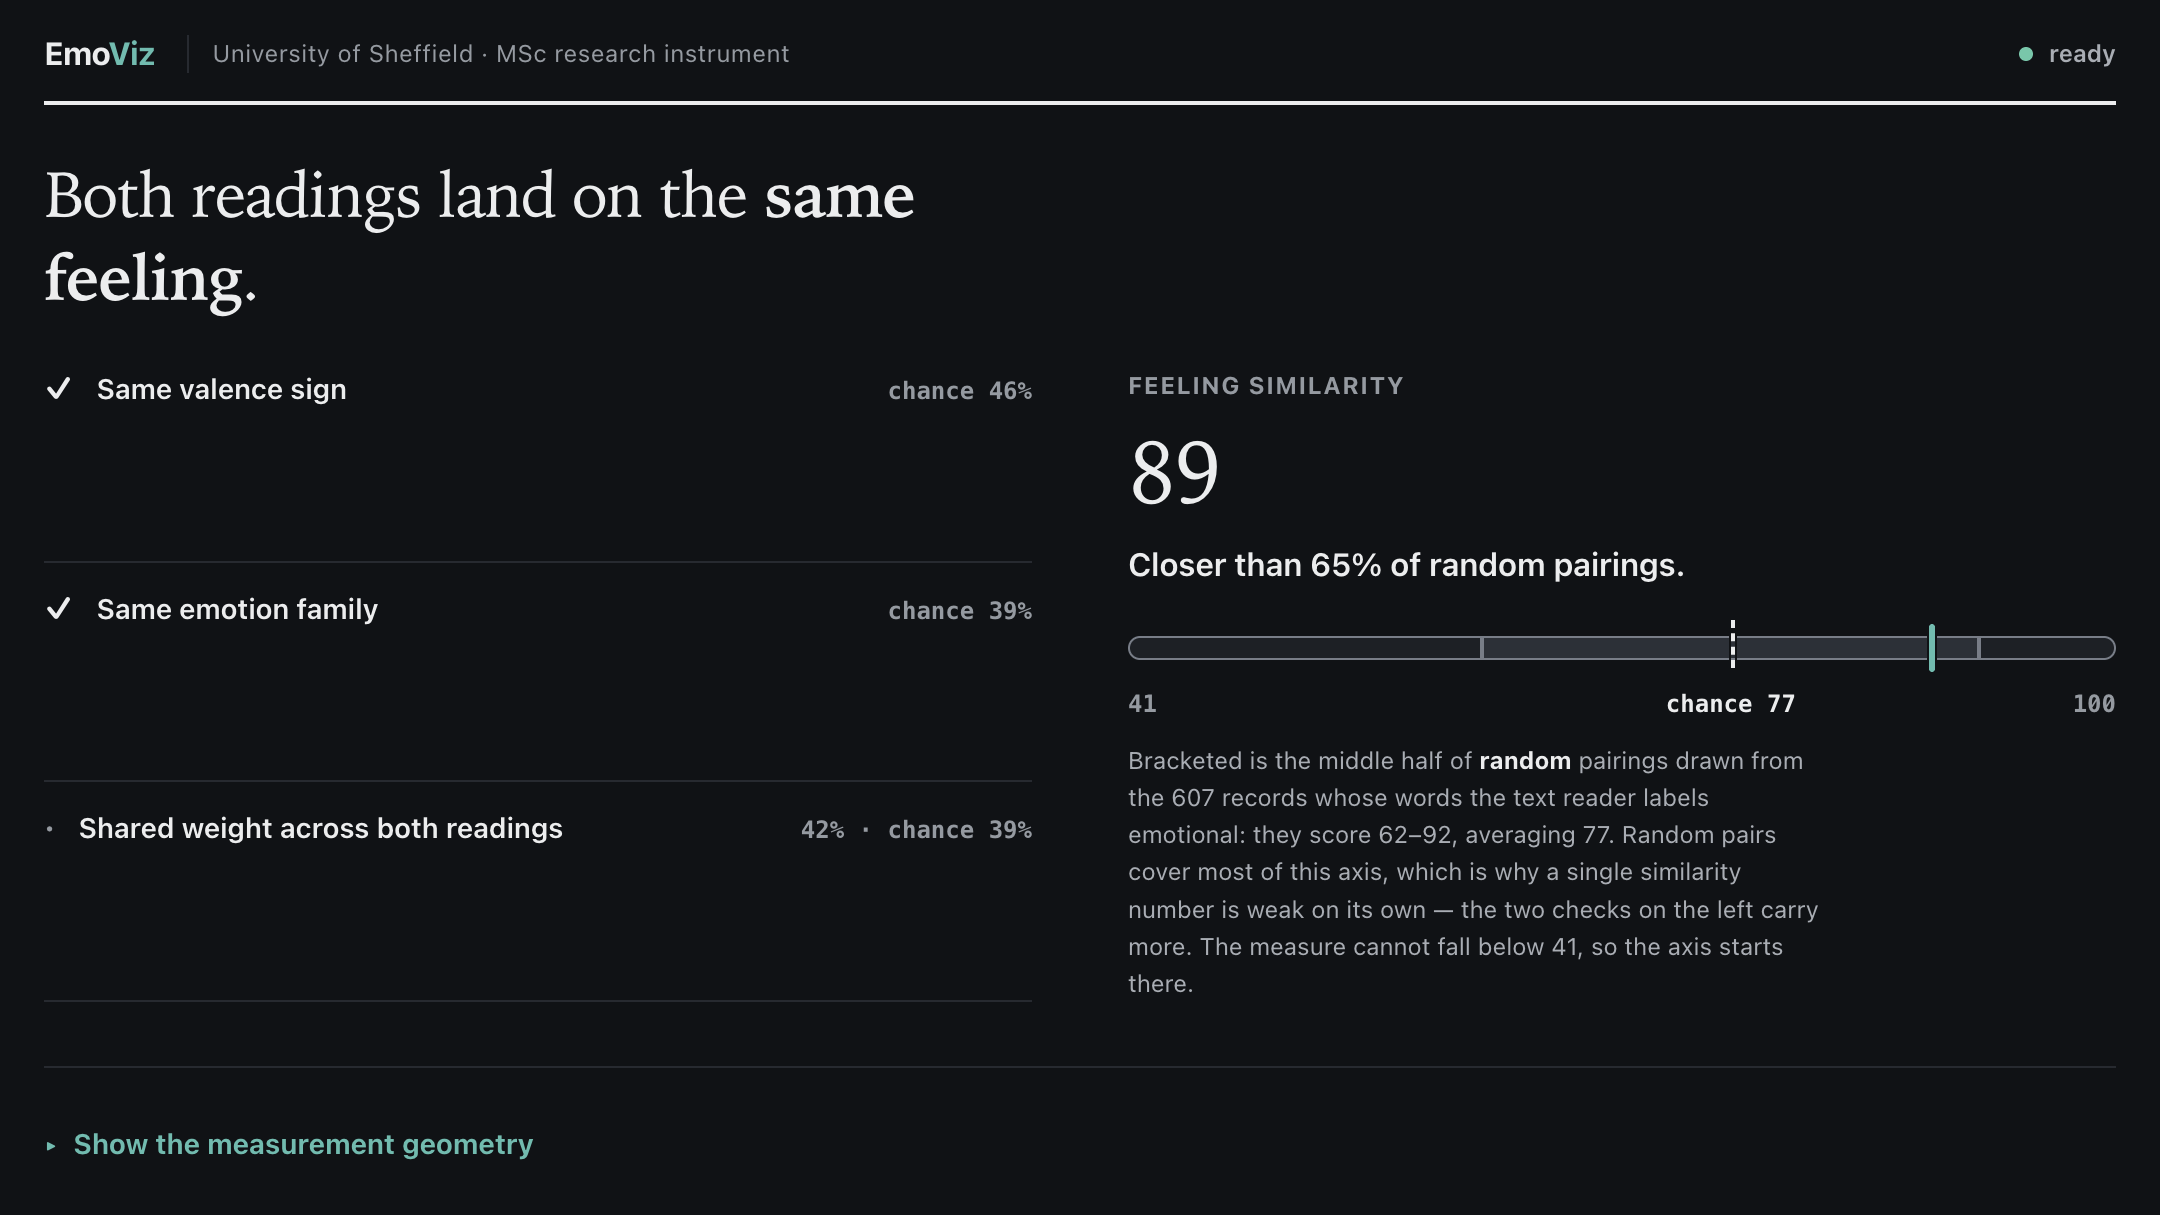
\includegraphics[width=0.9\textwidth]{demo_screenshot}
%   \caption{...}\label{fig:demo}\end{figure}
\newcommand{\placeholderfigure}[3]{%
\begin{figure}[htbp]
\centering
\begin{tcolorbox}[enhanced,width=0.92\textwidth,height=5.2cm,valign=center,halign=center,
  colback=black!3,colframe=white,boxrule=0pt,arc=2pt,borderline={0.9pt}{0pt}{black!50,dashed}]
\textbf{[ADD IMAGE HERE]}\\[5pt]
\small #3
\end{tcolorbox}
\caption{#2}
\label{#1}
\end{figure}}

\begin{document}

\frontmatter

\begin{titlepage}
\begin{center}

\includegraphics[width=5cm]{images/UOSLogo_Portrait_Violet_RGB.png}\\[2cm]
\linespread{1.2}\huge {\bfseries Visualising Emotion: A Similarity-Based Analysis of Emotional Fidelity in Text-to-Image Generation}\\[2cm]
\linespread{1}
{\Large Shre Hari Prem Anandh}\\[1cm]
{\large \emph{Supervisor:} Dr Chaona Chen}\\[1cm]
\large \emph{A report submitted in fulfilment of the requirements}\\ \emph{for the degree of} MSc in Artificial Intelligence\\[0.3cm]
\textit{in the}\\[0.3cm]
School of Computer Science\\[2cm]
September 2026
\end{center}
\end{titlepage}

% -------------------------------------------------------------------
% Declaration
% -------------------------------------------------------------------

\newpage
\chapter*{\Large Declaration}

\setstretch{1.1}

All sentences or passages quoted in this report from other people's work have been specifically acknowledged by clear cross-referencing to author, work and page(s). Any illustrations that are not the work of the author of this report have been used with the explicit permission of the originator and are specifically acknowledged. I understand that failure to do this amounts to plagiarism and will be considered grounds for failure in this project and the degree examination as a whole.\\[1cm]

\noindent Name:\\[1mm]
\rule[1em]{25em}{0.5pt}

\noindent Signature:\\[1mm]
\rule[1em]{25em}{0.5pt}

\noindent Date:\\[1mm]
\rule[1em]{25em}{0.5pt}

% -------------------------------------------------------------------
% Abstract, glossary
% -------------------------------------------------------------------

\chapter*{\Large \center Abstract}

Visitors to Sheffield's Festival of the Mind typed how they felt and a text-to-image installation answered each entry with a monochrome line drawing. That left \nTotal{} unlabelled prompt--drawing records, of which I analyse \nAnalysed{}. Nobody rated the drawings, so there is no ground truth. I ask instead whether one model's reading of a drawing agrees with another model's reading of its prompt. The prompt reader is RoBERTa fine-tuned on GoEmotions. The image reader is describe-then-extract, where BLIP-VQA is asked five factual questions and BART-MNLI reads an emotion family from the resulting description. On my supervisor's advice the readings are scored on a four-rung similarity ladder, from valence--arousal similarity to family agreement, and never matched label to label. Because valence--arousal similarity cannot fall below 0.412, with random pairs averaging \FullNeuVaNull{}, every score is reported beside its random-pairing null, and because \nRepeats{} records repeat a prompt, the intervals and tests are clustered on prompt groups.

On the \nEmotional{} prompts the prompt reader labels emotional, observed valence-sign agreement is \FullEmoSignObs{} where random pairing averages \FullEmoSignNull{} ($z$ = \FullEmoSignZ{}), and family agreement is \FullEmoFamObs{} against \FullEmoFamNull{}. Both hold with each prompt counted once and after Holm correction. Under the describer's split, face-classified drawings reach \FullFaceSignObs{} on valence sign and scene-classified drawings reach \FullSceneSignObs{}, a gap of \DiffSignPp{} (clustered 95\% interval \DiffSignCi{}, clustered permutation $p$ = \DiffSignP{}). Neutral-labelled prompts stay at chance. I also ran direct CLIP like for like; it gets \McClipFam{} family agreement where describe-then-extract gets \McDeFam{}. Where a prompt repeats, \ConsFam{} of its drawings receive the group's modal family, against \ConsFamNull{} with families shuffled.

The describer reports no person in \DescScenePeopleZero{} scene-classified drawings yet gives an expression for \DescScenePeopleZeroExpr{} of them, and corpus-wide, wherever that answer is an emotion word, the image reader returns that word's family \DescCopyStrict{} of the time. Dropping the expression sentence cuts valence-sign agreement to \AblDropExpressionEmoSignObs{} (null \AblDropExpressionEmoSignNull{}), and a people-aware template leaves the face rows unchanged and the scene rows at chance, so the headline agreement is a property of the measurement chain. To say what a person sees, I would need the single-coder check, then a human-rated study. The check was unscored when I wrote this. The dissertation contributes the corpus and the research question, the null-referenced ladder, the consistency experiment, and an audited, reproducible toolkit and demonstrator.

\chapter*{Glossary}
\addcontentsline{toc}{chapter}{Glossary}

% Fixed project vocabulary. The same words are used throughout the text.

\begin{description}\setlength{\itemsep}{2pt}
\item[Record] One prompt paired with the drawing made from it. Records are not linked to people. \nTotal\ were processed and \nAnalysed\ analysed.
\item[Prompt] The words a visitor typed. Prompts are quoted exactly as typed, lower case included.
\item[Drawing] The black-and-white line drawing the installation returned for a prompt.
\item[Prompt reader] The text model that reads the prompt: a RoBERTa model fine-tuned on GoEmotions (28 categories), summed into seven families.
\item[Describer] The vision model that answers five factual questions about a drawing (BLIP-VQA). It is never asked for an emotion.
\item[Image reader] The text model that infers a family from the describer's one-sentence description (BART-MNLI, zero-shot).
\item[Describe-then-extract] The image side of the pipeline: describer, template, image reader.
\item[Direct CLIP] The comparison reader, an OpenCLIP model asked for a family directly. Called the baseline; nothing else is.
\item[Category] One of the 28 GoEmotions labels.
\item[Family] One of seven groups the categories are summed into: joy, sadness, anger, fear, surprise, disgust, neutral.
\item[Agreement] The quantity this dissertation measures: how similar the prompt reader's reading of the words is to the image reader's reading of the drawing. It describes two machine readers and says nothing about what a person would see.
\item[Valence sign] $+$ for joy; $-$ for sadness, anger, fear and disgust; $0$ for surprise and neutral. Valence-sign agreement is computed over records whose prompt family has a sign.
\item[Family agreement] The share of records on which the two readers' top families coincide.
\item[Top-3 soft overlap] The overlap of the two readers' top-3 distributions once each is normalised to sum to one.
\item[Valence--arousal similarity] One minus the normalised distance between the two readings' score-weighted centroids on the circumplex. Its floor over the family centroids is 0.412, and randomly paired records already average about \FullNeuVaNull.
\item[Random-pairing null] The mean and spread a measure takes when the image readings are re-paired with the prompts at random (\nullShuffles\ re-pairings, seed \nullSeed). Every reported value is read against it.
\item[$z$] (observed $-$ null mean) / null standard deviation. Used to order effects, not as a precise probability: across seeds it moves by about a unit (\ZSeedMin\ to \ZSeedMax\ for the headline).
\item[Degenerate null] A null with zero spread. It arises when every prompt in a subset shares one label, so re-pairing cannot change the score. No $z$ is reported for it.
\item[Prompt group] All records whose prompt text is identical after case-folding, computed before redaction. There are \nDistinct\ groups; \nRepeats\ records repeat an earlier prompt. Every interval and test clusters on the group.
\item[Repeat group] A prompt group with two or more records (\nGroups\ of them, \nGroupRecords\ records).
\item[Clustered bootstrap] Resampling prompt groups, with replacement, to get 95\% confidence intervals that respect repeated prompts (\DiffDraws\ draws).
\item[Face-classified / scene-classified] A record is face-classified when the describer reports at least one person \emph{and} its expression answer contains a readable expression word. Every other record is scene-classified. The split is the describer's, not a person's.
\item[Emotional / neutral-labelled prompt] A prompt is emotional when the prompt reader's top family is not neutral (\nEmotional\ records); otherwise it is neutral-labelled (\nNonEmotional). The label was never checked by a person.
\item[Specificity check] The expectation that neutral-labelled prompts show no agreement above their null. Only valence--arousal similarity can move there.
\item[Copy rate] Where the describer's expression answer is itself an emotion word, the share of records in which the image reader's top family is that word's family (\DescCopyStrict\ on the strict definition).
\item[Consistency] For repeat groups, the mean share of drawings in a group that the image reader gives the group's most common family, read against a permutation null.
\item[People-aware template] The ablation variant of the description template that leaves out the person and expression clauses wherever the describer reported no people.
\item[Single-coder check] The 120-drawing sample the author codes blind, from contact sheets, to score the describer and the image reader against a person.
\item[Demonstrator] The local web application that runs the real pipeline on any record or an uploaded image and shows every measure against its chance level.
\end{description}


% -------------------------------------------------------------------
% TOC etc
% -------------------------------------------------------------------

\tableofcontents
\listoffigures
\listoftables

\setstretch{1.1}

\mainmatter

\chapter{Introduction}
\label{ch:intro}

\section{Context}
\label{sec:intro-context}

In September 2024 the University of Sheffield held its Festival of the Mind, and at one installation visitors were asked to type in how they felt. Whatever they typed went straight to DALL$\cdot$E, the model named in each file's provenance data, and the line drawing that came back, in black and white, went up on the screen for the visitor. There are \nTotal{} of these prompt--drawing records in all. They reached me when the project began in June 2026 as a folder of PNG files and a single JSON file of bare strings, without labels or metadata and with nothing to say who had typed what. The project specification offered a text strand and an image strand and left the focus to me.

Two features of the material shaped the work. First, the entries are short, and most of them are about the writer. The median length is four words, and 294 of the analysed records consist of one word only. The word ``happy'' by itself was typed \nHappy{} times, and other common entries are ``curious'', ``ok'', ``excited'' and ``good''. Many entries name more than one feeling at once, often feelings that pull against each other, as in ``tired but happy'' or ``tired proud happy'', and ``tired'' turns up inside many of the longer entries. A single label would lose part of what such an entry says. Second, every drawing is monochrome. The installation software appended a line-art instruction to each prompt (the instruction itself is not part of the data), so colour, which the literature treats as the main carrier of emotion in generated images \cite{alvarado2025texttoimage}, is missing from all \nTotal{} drawings. Whatever an automatic reader can recover from them has to come from line, posture, faces and composition.

The interface accepted any text at all. Some entries are not about a feeling at all: ``pigs'', which appears repeatedly, ``mickey mouse'', ``disney characters'', ``i like football'', and questions put to the machine such as ``how can a circle be squared''. Nothing ties a record to a person, so someone could have typed once or come back several times, and how many people contributed is unknown. Since \nRepeats{} of the \nAnalysed{} records repeat an earlier prompt, the count of contributors is at most \nDistinct{}, the number of distinct prompts. Every count in this dissertation is therefore a count of records. Figure~\ref{fig:examples} gives six records in the form used throughout this dissertation, the visitor's words with any personal name replaced by a placeholder, next to the drawing made from them.

\begin{figure}[htbp]
\centering
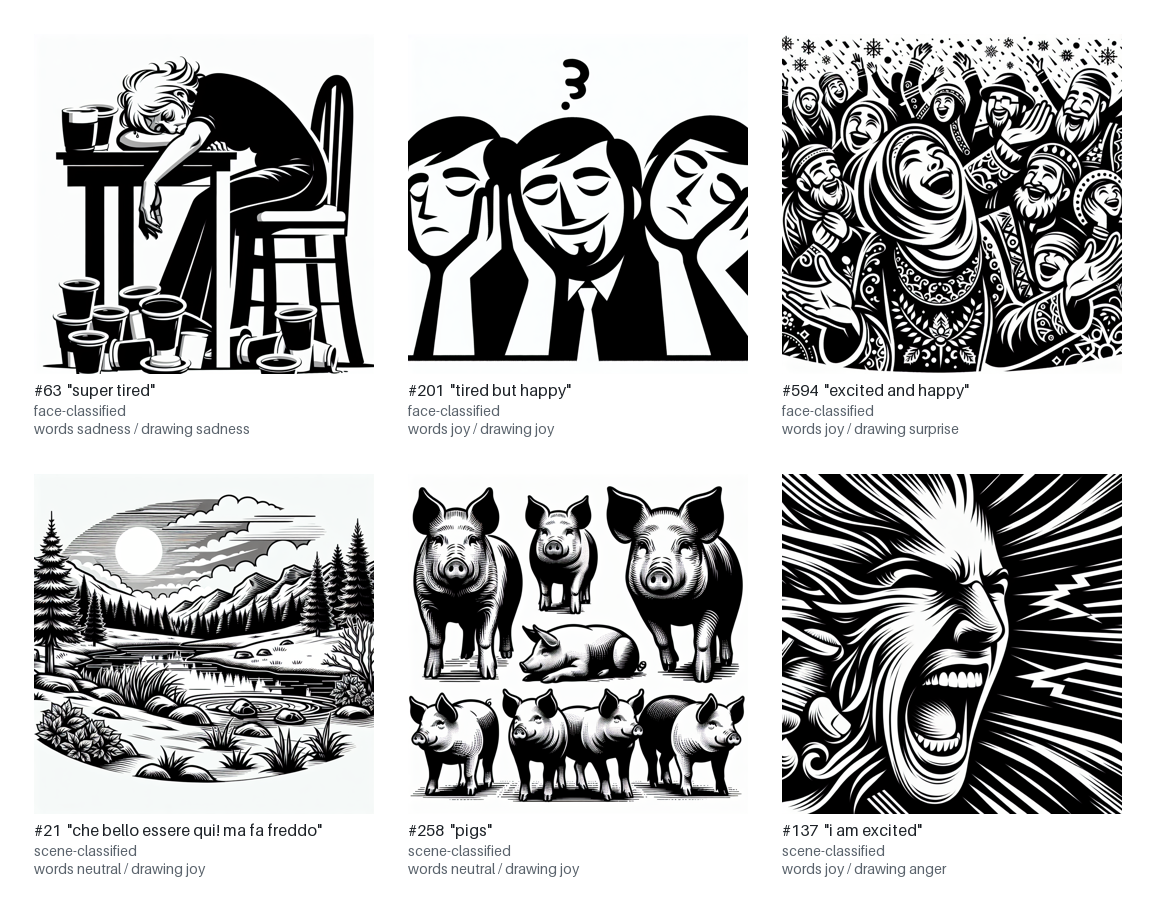
\includegraphics[width=\textwidth]{examples}
\caption{Six records as they appear throughout this dissertation. Under each drawing are the record number, the prompt as typed, the class the describer assigned (face or scene, Section~\ref{sec:method-pipeline}) and the family returned by each of the two readers. The demonstrator examples (Section~\ref{sec:method-demo}) are records 63 and 201. In record 21 the drawing is of mountains, the describer reported no people, and its expression answer was still ``smiling''; Section~\ref{sec:results-describer} reports how often that happens.}
\label{fig:examples}
\end{figure}

\section{The question}
\label{sec:intro-question}

If someone types something about how they feel and an image generator draws it, how far does the emotion read from the words agree with the emotion read from the drawing? That is the research question, and the data limit how it can be answered. Nobody rated these drawings, and the only record of what a visitor meant is what the visitor typed. Each side therefore gets an automatic reader in place of a person. A language model assigns the prompt an emotion, and a second reader does the same for the drawing by first putting it into words and then reading those words. All the numbers reported here are agreement between those two readings. What a person looking at a drawing would see is a separate question that needs human raters, and Chapter~\ref{ch:conclusion} lists that study as further work.

The design follows a direction my supervisor gave at a meeting at the end of July. Dr Chen is a psychologist who works on facial expressions, and her point was that scoring a drawing as a hit or a miss against a label is too crude for emotion. Two people looking at the same face will often not agree about what it is doing, and the models are noisy on top of that. The labels overlap as well. Cowen and Keltner \cite{cowen2017self} found 27 categories in self-reported experience, joined to one another by continuous gradients, and on Russell's circumplex \cite{russell1980circumplex, posner2005circumplex} ``happy'' lies a short distance from ``excited'' on the valence--arousal plane. If a visitor typed ``happy'' and the drawing is read as excited, counting that as a complete miss throws away most of what this corpus has to offer. So the project asks how similar two readings are, and it never scores a drawing on whether it matches a label. Dr Chen asked for this similarity framing to be named as the novel element of the work.

In place of the hit-or-miss score there are four measures arranged as a ladder, from loose to strict, and each is compared with what comes out when drawings are paired with prompts at random. Chapter~\ref{ch:method} defines them. Valence--arousal similarity is the loosest and family agreement, which needs the two top families to coincide, is the strictest; top-3 soft overlap and valence-sign agreement sit between them. The chance reference is needed because the loosest measure does not start at zero. Valence--arousal similarity has a floor of 0.412 on a scale whose top is 1, and a random pairing of drawings with prompts already scores about \FullNeuVaNull{}, so a value that looks respectable at first sight can sit below chance. I ran into this while building the demonstrator, when a value that looked fine on screen was in fact under the random-pairing mean.

\section{Aims and objectives}
\label{sec:intro-aims}

The aim is to measure how closely two automatic readers, one reading the visitor's words and the other the drawing, agree about the emotion in a record, with each value set against its chance level, and to describe the instrument well enough that its weak points are on record. There are eight objectives.

\begin{enumerate}
\item Build the image side as a describe-then-extract pipeline, in which a vision model answers factual questions about the picture and a separate text model reads an emotion from those answers, so that the vision model is never asked about emotion.
\item Define the four-rung similarity ladder and the random-pairing null, so that no value is reported without its chance level.
\item Measure agreement on the full corpus and then separately on the two splits Dr Chen asked for: emotional prompts against neutral-labelled ones, and face-classified drawings against scene-classified ones.
\item Put the face/scene difference to a formal test, and check that the headline results are not an artefact of the repeated prompts.
\item Run a like-for-like comparison between describe-then-extract and a direct CLIP reader, with both given the same records, the same prompt-side readings and the same measures.
\item Turn the repeated prompts into a consistency measurement, asking how far drawings made from one and the same prompt are given the same family by the image reader.
\item Audit the instrument. The checks are a control audit of the neutral-labelled prompts, an audit of the describer's answers, a taxonomy of the strongest disagreements by failure mode, a single-coder check on a blind sample of drawings, and an ablation over the description template.
\item Release the toolkit in a reproducible form, with the headline numbers pinned by tests and a demonstrator that runs the real models.
\end{enumerate}

\section{Contributions}
\label{sec:intro-contributions}

Very little of the software is new in itself. The prompt side uses RoBERTa fine-tuned on GoEmotions, the image side uses a visual question-answering model followed by a natural-language-inference model, and the inference relies on textbook procedures such as the clustered bootstrap and the permutation test. The new parts are the object of study and the question put to it, the practice of setting every answer against its chance level, the consistency experiment, and the audits.

The material is new because nobody gave the visitors a list of emotions to pick from or a template to fill in, and what they typed is mostly short self-reports from members of the public, many naming more than one feeling, each drawn as a line drawing with no colour in it. The closest prior study is by Lomas and colleagues \cite{lomas2024improved}. Their design differs on several points: ten emotions from a fixed list, each generated on a person or a robot, in colour, and scored by human raters. None of the 73 papers retained for the review in Chapter~\ref{ch:lit} measures agreement between the emotion read from a short, mixed self-report and the emotion read from a colour-free drawing made of it.

For each record the question is whether the two readings agree end to end, and it is answered with the ladder set against its null. Because \nRepeats{} records repeat a prompt and cannot be treated as independent, the intervals are clustered on prompt groups, and the one contrast the design was built around, face-classified against scene-classified drawings, gets a formal permutation test. The repeated prompts also allow a consistency experiment. It needs the same words drawn more than once, which none of the studies reviewed in Chapter~\ref{ch:lit} had, and it measures how often the image reader gives the same family to a prompt drawn again.

The audits put numbers on the instrument's weak points: how far the image reading depends on a single word from the describer, what the describer answers when the drawing has no face in it, how many of the neutral-labelled prompts contain a plain affect word after all, and how many of the strongest disagreements can be traced to the generator as against the readers. Until the second audit in September the scene drawings looked as if they sat a little above chance. The template ablation in that audit removed that result (Chapter~\ref{ch:results}).

In practical terms the deliverables are the analysis code, the result tables over the \nAnalysed{} records, the demonstrator, a two-layer test suite and the audits themselves. The demonstrator is a small Flask application, run locally, that puts any analysed record or an uploaded image through the real models and reports all four measures against the chance levels the analysis uses. One test layer is a shell script that checks the environment, the corpus files and the cached model outputs, then runs the live pipeline over a few fresh images; the other pins each headline number to the JSON file behind it. Each statistic in the text is a LaTeX macro produced from those same result files. Re-running the analysis rewrites the numbers here without anyone retyping them.

\section{Overview of the report}
\label{sec:intro-overview}

The literature review in Chapter~\ref{ch:lit} goes through eight themes, from theories of emotion to how the public receives pictures made by AI, and closes by stating the gap the project sits in. Chapter~\ref{ch:method} covers the corpus and its pre-processing, then the two readers, then the ladder with its null and the inference procedures, then each analysis, the demonstrator and the alternatives I tried first and dropped. The numbers, with their tables and figures, are in Chapter~\ref{ch:results}. Interpretation is held over to Chapter~\ref{ch:discussion}, which sets out what the results do and do not establish, why the weakest part of the chain is the describer, and how the findings sit next to earlier work. Chapter~\ref{ch:conclusion} closes with further work in the order the evaluation points to. Three appendices follow. Appendix~\ref{app:repro} gives the layout of the repository, the order in which the scripts run and the pinned environment. Appendix~\ref{app:instruments} collects the fixed strings the pipeline depends on: the five describer questions, the description template, the hypothesis string, the expression-word list, the category-to-family map, the circumplex centroids, the coder's instructions and the redaction procedure. The record of supervision meetings is Appendix~\ref{app:supervision}.
   % Introduction
\chapter{Literature Review}
\label{ch:lit}

\section{Scope and method of the review}
\label{sec:lit-scope}

Five bodies of work bear on this project, and few papers cite across them. The psychology of emotion, emotion detection in text, image generation from text, the scoring of generated pictures, and the study of how people judge feeling in a picture each have something to say about a drawing made from the words ``tired but happy''. All five were read across to check that none of them had already asked this project's question. The starting point was the eight papers Dr Chen provided when the project began. From each of those the reference lists were followed outward, one literature at a time. Ninety-seven papers were read in full.

Every paper got two scores, one for how close it sat to the path of the dissertation and one for the strength of its evidence, and a paper was kept only when it did well on both. In practice that meant an empirical study with an evaluation of its own, or a dataset, lexicon or benchmark that later work builds on. Surveys and position pieces went out. So did careful work that was aimed somewhere else, and a reason was logged for every exclusion, so that the 24 papers dropped at this stage can be checked against the criterion. Two foundations would have failed the evidence test applied strictly, Ekman on basic emotions and Russell on the circumplex, and they were kept regardless, because every classifier and every lexicon further down assumes one or the other. That left 73 papers, and they fell into eight themes. On 9 September, after the second audit, 18 references were added for the models and the statistical procedures that the methodology depends on, which takes the bibliography to 91 entries; they are cited where they are used, here and in Chapter~\ref{ch:method}. The eight themes give this chapter its sections.

One term needs settling before the review starts. When other people's papers discuss how well an image corresponds to its prompt they say \emph{alignment}, and their term is kept here whenever their work is described. For this project the word is \emph{agreement}. What is measured here is how often two readers, one given the prompt and one given the drawing, return the same thing, and calling that alignment would imply a standard that the drawing either meets or misses, and this corpus has no such standard.

\section{Foundations: emotion theory and taxonomy}
\label{sec:lit-theory}

The vocabulary comes from two traditions. Ekman \cite{ekman1992argument} made the case that a small number of basic emotions exist, each with its own signal, and the six-way scheme that most classifiers still use is his: happiness, sadness, anger, fear, surprise and disgust. Russell's circumplex \cite{russell1980circumplex} puts affect on two continuous axes instead, valence and arousal, and the later paper by Posner, Russell and Peterson \cite{posner2005circumplex} argues from neural and developmental evidence that the dimensional picture fits better than the categorical one. Both are used here. The seven families in this dissertation, Ekman's six with neutral added, form the categorical rung, and the dimensional rung comes from where each family sits on the circumplex.

Neither scheme on its own covers what people report. Cowen and Keltner \cite{cowen2017self} asked people what they felt while watching more than two thousand brief video clips, and the reports resolved into 27 distinct categories linked by continuous gradients; the categories explained more of the variance than valence and arousal did, and neither description was enough by itself. The similarity framing rests on this result. If ``happy'' and ``excited'' lie next to each other on a gradient, then a rule that counts a drawing read as excited as a complete miss for a prompt that said happy is really measuring where the boundaries of the label set fall.

The same point has been made for faces in Dr Chen's own field. Using reverse correlation, Jack and colleagues showed that Western and East Asian observers do not hold the same mental representations of the six basic expressions \cite{jack2012facial}. A later study found that the signals in a dynamic expression arrive in a hierarchy over time, so that the early movements reduce six emotions to four, fear being confusable with surprise and disgust with anger at the start \cite{jack2014dynamic}. Dr Chen and her colleagues found distinct facial signatures for pain and for pleasure inside each culture \cite{chen2018distinct}. They then moved psychologically valid expressions onto social robots and a conversational virtual agent by measuring what observers reported seeing in a face \cite{chen2018reverse, chen2020building}. Their most recent work finds that facial movements code the category of an emotion and its intensity as separate components \cite{chen2024cultural}.

For a project that reads emotion off drawn faces, this has consequences. There is no reference drawing of an emotion to compare against, and near misses between neighbouring categories are to be expected. What a face signals is settled, in this tradition, by what human observers report, which this project does not measure because both of its readers are programs. So the foundations settled two design decisions, a small family scheme that two quite different readers can both output and a dimensional measure beside it, so that a drawing read as excited for the prompt ``happy'' earns partial credit.

\section{Emotion from text}
\label{sec:lit-text}

Text emotion recognition has mostly been built and tested on longer social-media text, and it is weakest on short first-person entries like the ones in this corpus. The reference resource is GoEmotions \cite{demszky2020goemotions}: 58,000 Reddit comments, each annotated with one or more of 27 fine-grained categories or with neutral, together with a mapping from those categories onto Ekman's families that the authors themselves propose and that this project uses. Their BERT (Bidirectional Encoder Representations from Transformers) model's macro-F1 was 0.46. The average hides a lot, because the score falls towards zero on the rare categories whose emotion is implied and never named. Harutyunyan and Kumar \cite{harutyunyan2026fine} re-ran the comparison on the same data across classical learners, a recurrent network and transformers, and the same shape appears in every row. Yang and colleagues \cite{yang2023context} used large language models to audit emotion datasets and found short texts under-specified as a rule; the label frequently turns on context that the text leaves out. A festival entry is that case, since it is written in the first person and is a few words long, and it often names two feelings.

Two papers take short texts on directly: Liu and colleagues \cite{liu2023emotion} propose an improved multi-label method for them, and Bhat \cite{bhat2024emotion} reports that a small transformer classifies short English texts well. Both were built and tested on tweets, though, and a tweet still gives the model more to work with than ``tired but happy'' does.

Dimensional resources go part of the way round the problem. EmoBank \cite{buechel2017emobank} rated ten thousand sentences on valence, arousal and dominance twice over, once from the writer's point of view and once from the reader's, and found that the two sets of ratings differ, which matters for this project because a visitor's words come from the writer's side and every reader in the pipeline sits, by construction, on the reader's side. The NRC lexicons supply valence, arousal and dominance norms at word level, first for twenty thousand English words \cite{mohammad2018obtaining} and now for fifty-five thousand \cite{mohammad2025nrc}, and the earlier crowdsourced lexicon \cite{mohammad2013crowdsourcing} maps words to basic emotions. Linguistic Inquiry and Word Count (LIWC) \cite{tausczik2010psychological} is still the transparent tool that psychologists reach for, a validated dictionary whose categories include positive and negative emotion, anxiety, anger and sadness. Zanwar and colleagues \cite{zanwar2022improving} found that fusing such psycholinguistic features with a transformer helps it generalise out of domain, which is a live worry for a corpus unlike anything the models were trained on. Niu and Mower Provost \cite{niu2025contrastive} compress what a large language model knows about emotion into a compact recogniser that needs no labelled examples. Parkington and colleagues \cite{parkington2025human} compared a large language model with expert human coders doing thematic analysis, and found high agreement between them but a loss of fine detail on emotional triggers. BERTopic \cite{grootendorst2022bertopic} was considered for pulling themes out of the corpus and set aside, because topic modelling has nothing to work with when the median document is four words long.

The rest of the text-side references are the models used in the pipeline. Entailment-based zero-shot classification \cite{yin2019benchmarking} turns each candidate label into a hypothesis sentence and puts it to a natural-language-inference model, which says whether the input entails it, and BART \cite{lewis2020bart} trained on MultiNLI \cite{williams2018broad} is the usual choice for that model and the one that reads the descriptions here. T5 \cite{raffel2020exploring} recast every task as text-to-text, its instruction-tuned successor \cite{chung2022scaling} extended that, and some of the vision--language models in Section~\ref{sec:lit-t2i} are built on the two of them. Everything runs through the Transformers library \cite{wolf2020transformers}.

On the text side the prompt reader is the least reliable part of the chain, and that shaped two choices. Its label on a four-word entry is uncertain, and every number downstream inherits the uncertainty. Chapter~\ref{ch:method} explains why GoEmotions was chosen over an entailment model and a hand-built lexicon for the prompt side; the short version is that it was trained on first-person Reddit comments, the nearest register to a festival entry available. The decision to keep the prompts that the reader labels neutral as a group of their own and analyse them, the specificity check of Chapter~\ref{ch:results}, comes from this literature too. A label of neutral on a two-word entry is exactly the kind of judgement Yang and colleagues warn about.

\section{Datasets, benchmarks and lexicons}
\label{sec:lit-data}

Every image-side resource in this literature is photographic or painted, and every one is in colour. EmoSet \cite{yang2023emoset} is the largest, at 118,000 images, each labelled with one of eight emotions and a set of attributes. Machajdik and Hanbury \cite{machajdik2010affective} built their affective classifier from colour, texture and composition features drawn from art theory, and they reported how far people agree with one another on the same images as a reference point. The Nencki Affective Picture System \cite{marchewka2014nencki} is a set of photographs that come with normative ratings of valence and arousal. EMOTIC \cite{kosti2020context} annotates people in their surroundings, with 26 categories as well as continuous dimensions, and its finding is that what surrounds a person changes which emotion annotators assign to that person. None of these resources contains line drawings, and that domain shift is one of the two reasons for the shape of the image side (the other, Dr Chen's direction, comes up in Section~\ref{sec:lit-t2i}). A classifier built on any of these resources could be run over the drawings, but its output could not be trusted, so the pipeline describes a drawing first and extracts the emotion from the description afterwards. The direct-CLIP reader is kept as the baseline that the method is compared against.

The art datasets come closest to this corpus because each pairs a picture with a short piece of affective text. ArtEmis \cite{achlioptas2021artemis} gathered 439,000 utterances in which annotators say what emotion an artwork makes them feel and why. ArtELingo \cite{mohamed2022artelingo} took the same paintings into four languages and found that the emotion labels move with the language and culture of the annotator. WikiArt Emotions \cite{mohammad2018wikiart} covers four thousand paintings and gave two results relied on later. Giving an image a title shifts the emotion people report for it. Images with a face in them get much more consistent emotion judgements from annotators than images without one. On the text side, CARER \cite{saravia2018carer} built a tweet corpus by distant supervision with eight emotions, and it is where the widely used ``emotion'' dataset comes from; the SemEval affect tasks from 2018 \cite{mohammad2018semeval} and from 2025 \cite{muhammad2025semeval} fix the shared benchmarks and the protocol for scoring intensity. Then there are the human-preference datasets built for text-to-image models, ImageReward \cite{xu2023imagereward}, Pick-a-Pic \cite{kirstain2023pick} and Human Preference Score \cite{wu2023human}, each of which records which of a pair of generated images people preferred, without asking about emotion, and trains a scorer on the answer.

\section{Text-to-image generative models}
\label{sec:lit-t2i}

The drawings were made by a DALL$\cdot$E model. The original DALL$\cdot$E \cite{ramesh2021zero} was a discrete autoregressive model, the second version \cite{ramesh2022hierarchical} decoded images by diffusion, conditioned on CLIP image embeddings, and DALL$\cdot$E~3 \cite{betker2023improving} trained on synthetic captions to follow prompts more closely and rewrites what the user typed before generating anything. Which of these made the festival drawings is not recorded. The provenance manifest inside each PNG names the software agent as ``DALL$\cdot$E'' and nothing more, with no version, no seed and no copy of the rewritten prompt. So no drawing can be produced again, and nothing about the generator by itself can be separated from the rest of the chain, a limit that returns in the consistency experiment. The diffusion models that DALL$\cdot$E sits beside, latent diffusion \cite{rombach2022high}, SDXL \cite{podell2023sdxl} and Imagen \cite{saharia2022photorealistic}, share a set of well-documented weaknesses: fine detail, rendered text and faces.

The readers used here are from the same few years. CLIP \cite{radford2021learning} learned to embed images and captions in one space from 400 million pairs of photographs and text, and it has become the default zero-shot image classifier. It was trained on colour photographs and its strength is objects, and for that reason Dr Chen's direction in late July was not to ask it for an emotion. Bootstrapping Language-Image Pre-training (BLIP) \cite{li2022blip} learned both captioning and visual question answering by bootstrapping from noisy web data; its VQA head takes an image and a free-form question and returns an answer, and the describer in this project does that five times per drawing. BLIP-2 \cite{li2023blip} joins a frozen image encoder to a large language model through a small trainable bridge. OpenCLIP \cite{ilharco2021openclip} is the open re-implementation of CLIP, and it is the model behind the direct-CLIP baseline. All of these readers are borrowed instruments, picked for what each is good at, and the choice to put a question-answering describer in front of the emotion reader, instead of a classifier, follows from the domain-shift argument of Section~\ref{sec:lit-data}.

\section{Image evaluation: metrics and frameworks}
\label{sec:lit-eval}

Automatic scoring of text-to-image models has settled on one question, whether the objects, attributes and relations that the prompt named are present in the picture. CLIPScore \cite{hessel2021clipscore} is the cosine similarity of the CLIP embeddings for the image and for the text. TIFA \cite{hu2023tifa} turns the prompt into questions and lets a VQA model answer them against the image. Cho and colleagues' Davidsonian Scene Graph \cite{cho2024davidsonian} orders those questions so that a dependent question is only asked once its premise has been confirmed. GenEval \cite{ghosh2023geneval} runs an object detector and checks counts, colours and positions. VQAScore \cite{lin2024evaluating, li2024evaluating} puts one yes/no question to a generative vision--language model, takes the probability of ``yes'' as the score, and on the human ratings of GenAI-Bench it tracks people far more closely than CLIPScore does. The Conditional Fr\'echet Distance \cite{koo2026evaluating} compares a model's output distribution with a reference distribution, conditioned on the prompt. Behind these sit the caption metrics that came first, SPICE \cite{anderson2016spice} and CIDEr \cite{vedantam2015cider}, and the Fr\'echet Inception Distance (FID) \cite{heusel2017gans}, which scores image quality without looking at the prompt.

How much any of this can be trusted is answered by two studies. Lee and colleagues \cite{lee2023holistic} evaluated text-to-image models on many axes at once and found that the automatic scores agree only weakly with human ratings on several of them, including photorealism and aesthetics. Zhang and Wan \cite{zhang2025rethinking} put CLIPScore, VQAScore and DSGScore under stress on a set of about a thousand prompts, which is roughly the size of this corpus, and the first and the third reversed the ranking of models when the seed changed and moved materially after a single pixel was perturbed. VQAScore was steadier, though not immune.

A second group of papers looks at the judge instead of the score. Chang and colleagues \cite{chang2023prompt} describe the way experienced prompt artists push a model towards a style with keywords such as ``black and white'' and ``line art'', and note that an output drifts towards the model's average look unless it is pushed. Oppenlaender and colleagues \cite{oppenlaender2024artworks} report that driving generation from a body pose changes the feeling of the resulting image without anyone intending it, and that uncanny artefacts change how the image is read emotionally. Carrasco and colleagues \cite{carrasco2024level} asked how closely human raters' labels follow the emotion a generator had been told to produce, scored it with Cohen's kappa and Krippendorff's alpha, and found the agreement much stronger once the labels were reduced to positive and negative. Across ten experiments, Horton, White and Iyengar \cite{horton2023bias} together with Millet and colleagues \cite{millet2023defending} find that people rate the same piece of work lower when they are told a machine made it, which constrains the design of any later human study on these drawings. Two benchmarks test the machine judges themselves. Bhattacharyya and Wang \cite{bhattacharyya2025evaluating} found that vision--language models do a poor job of recognising, zero-shot, the emotion an image evokes in a viewer, lean systematically towards positive labels, and change their answer with the order in which the candidate labels are listed. Gao and colleagues \cite{gao2025eemo} report that multimodal models manage valence, fail on arousal and dominance, and run together what the person in the picture expresses and what the person looking at it feels.

No alignment metric measures affect, so none of them could be the instrument here, although VQAScore, which works by asking a question and reading the answer, is the nearest relative of the describer used here. They are also unstable. Because the scores move with the seed and with a single pixel, no value in this dissertation is reported bare, and each is compared with its random-pairing null. The positive lean and the expressed-versus-evoked confusion that the two benchmarks found in machine judges are the failure modes the audits in Chapter~\ref{ch:results} check for, and both appear in this corpus.

\section{The intersection: emotion in generated images}
\label{sec:lit-intersection}

The papers that put emotion into generated images condition on a target and work in colour. EmoGen \cite{yang2024emogen} generates an image from an emotion category by way of an emotion space mapped onto CLIP's, and scores the result with an EmoSet-trained classifier. Make Me Happier \cite{lin2024make} takes an existing image and edits it towards a chosen emotion; its authors found positive emotions harder to separate from each other than negative ones, and fine facial detail was a weak point. EmotiCrafter \cite{dang2025emoticrafter} conditions generation on a continuous valence--arousal coordinate. Mehta and Buntain \cite{mehta2024generating} asked whether generators drift towards fear whatever the prompt says, with an image-emotion classifier for the pictures and a text-emotion classifier for the prompts, and that cross-modal design is the nearest methodological relative of the pipeline here. Zhou and colleagues \cite{zhou2025analyzing} turn an image into affective captions first and classify the evoked emotion from those, so the describe-then-extract idea has a precedent on the recognition side too.

Alvarado \cite{alvarado2025texttoimage} had a diffusion model render emotion words and then extracted colour features from what came back, and found that lightness and chroma track emotional meaning in the output more closely than hue does. Only colour features are modelled. Shape and line are not tested, so the study says nothing either way about what a drawing with no colour in it can do. The literature therefore offered no prediction for a corpus without colour, which is one reason it seemed worth studying.

The nearest prior study is by Lomas and colleagues \cite{lomas2024improved}. Twenty-four raters scored 240 images, made by three generators from a fixed list of ten emotions, with each emotion rendered on a person or on a robot, rating alignment from 0 to 10. The generating model was the largest effect, with DALL$\cdot$E~3 well ahead of Stable Diffusion and of DALL$\cdot$E~2, and the scores differed sharply from one emotion to the next; emotions rendered on a person scored higher than the same emotions on a robot. Their prompts were built from a template and their images were in colour. Nobody, in the papers reviewed, has measured affect agreement for self-reports that came straight from the public, mixed feelings included, and were drawn without colour. None of these studies drew the same words twice either, so none could ask how stable a reading is, and the repeated prompts in this corpus make that question possible.

\section{Emotion perception and human judgement}
\label{sec:lit-perception}

Machine recognition of emotion in pictures was built on photographs, and it mixes up two different constructs. Yang and colleagues \cite{yang2018weakly} learned visual sentiment with a pair of coupled networks and weak supervision. EmoSet and the other datasets of Section~\ref{sec:lit-data} supply the labels such systems learn from, and the benchmarks in Section~\ref{sec:lit-eval} show how brittle the resulting judges are. Underneath this is a distinction, formalised by Gao and colleagues \cite{gao2025eemo} and made concrete in Dr Chen's experiments, between what the person in a picture expresses and what a viewer feels on looking at it. A classifier fitted to crowd labels returns a mixture of the two. The pipeline here reads expressed cues only. It works from a drawn expression, a posture and an action. A study with human raters would be reading evoked affect, and the two cannot be pooled. The reverse-correlation methods that Jack and Dr Chen have used \cite{jack2012facial, chen2018distinct, chen2020building, chen2024cultural} show how such a study should be run: start by measuring what observers report seeing, without presupposing it.

The distinction settles the vocabulary used from here on. What the image reader returns is called a reading throughout. Nothing in the computational results says what a person sees, because nobody looked at a drawing until the single-coder check of Chapter~\ref{ch:results}, and that check is the only point in the project at which somebody does.

\section{Context}
\label{sec:lit-context}

The drawings were made at a public festival. One study of how the public receives machine-made art bears on them directly. In a study of 565 participants, Ragot and colleagues \cite{ragot2020ai} found that an identical artwork is rated lower as soon as it is labelled as made by a machine. Every drawing here was shown to its author as machine-made, so anyone who rates them in future will have to hide that label or counterbalance it.

\section{The gap}
\label{sec:lit-gap}

Taken together, these literatures describe an object that none of them has studied. A short self-report holds blended, graded affect, and short first-person text is where emotion classifiers do worst. A generator renders such a prompt fluently but can falter on faces and fine detail, and it may not even draw the words the visitor typed. The strongest evaluation metrics count objects and are unstable in their own right, while the work on emotion in images reads affect mainly through colour, on photographs and paintings, using judges that lean positive and confuse the emotion a depicted person expresses with the emotion felt by the viewer.

Across the 73 papers, no study measures how far the emotion a reader recovers from a first-person self-report that is short, unmediated and mixed in affect agrees with the emotion a reader recovers from a colourless line drawing generated from it. No study asks, either, how stable that second reading is when the identical words are drawn a second time. A compositional metric can pass a line drawing on the question ``is there a person?'' and the reader can still return sadness for a prompt that read ``happy''. Lomas and colleagues used a fixed typology and coloured images, whereas the prompts here are whatever somebody typed, blends included, and the drawings are colourless. The conditional generators treat emotion as a control setting; here it is latent in a visitor's words. The visual-emotion recognisers were trained on photographs and paintings, so monochrome line art sits outside their training distribution, and not one of them keeps expressed and evoked affect apart for such stimuli.

The rest of the dissertation asks two questions. The first is how closely two automatic readers agree about the emotion in a visitor's words and in the drawing made from them, measured against chance, and how much of that agreement depends on whether the drawing has a readable face. The second is how stable the reading stays when one prompt is drawn several times. What a person looking at these drawings would see needs people to answer it and is left to further work. The dissertation's contribution is the corpus and the question, a similarity ladder with a chance level under every rung, a consistency experiment that the repeated prompts make possible, and an audited toolkit; it proposes no new metric or classifier.
   % Literature Review
\chapter{Methodology}
\label{ch:method}

\section{Overview and design principles}
\label{sec:method-overview}

Three decisions shaped this chapter more than any others. Two came from Dr Chen in late July and one from the demonstrator in August, and they are set out before following the data through the chapter in the order it is processed.

The first is that the comparison is one of similarity. Dr Chen's view was that, with emotion subjective, people in disagreement and models noisy, scoring a drawing as a match or a miss against one label would be too crude, and she asked for the similarity framing to be stated as the novel element. Each reader therefore returns a scored list over one set of seven families, and the two lists are compared on four measures arranged as a ladder, from a forgiving circumplex distance up to a strict test of the top family (Section~\ref{sec:method-measures}). All four rungs are reported together.

The second is that no value is quoted without its chance level. This one was not there from the start. While the demonstrator was being wired up in August it became clear that records paired at random already scored around \FullNeuVaNull{} on the loosest measure, since the seven centroids crowd into a small part of the plane and the lowest value the measure can take is 0.412. So 0.71 looks respectable and is under chance. From then on every cell of every table got a random-pairing null (Section~\ref{sec:method-null}); the clustered intervals and the test of the face/scene contrast came later, in the September audits (Section~\ref{sec:method-inference}).

The third is that the vision model is at no point asked about emotion. This too was Dr Chen's instruction, since CLIP learned from colour photographs and is good at objects. The describer answers five plain questions about what is drawn, a fixed template makes one sentence of the answers, and a second text model reads a family out of that sentence, so both sides of the comparison end up as text (Section~\ref{sec:method-pipeline}). How much independence that buys is measured in Section~\ref{sec:method-analyses}, and it is less than expected. Figure~\ref{fig:pipeline} shows the chain.

\begin{figure}[htbp]
\centering
\resizebox{\textwidth}{!}{% TikZ: the describe-then-extract pipeline and the similarity ladder. Input from chapter3.tex.
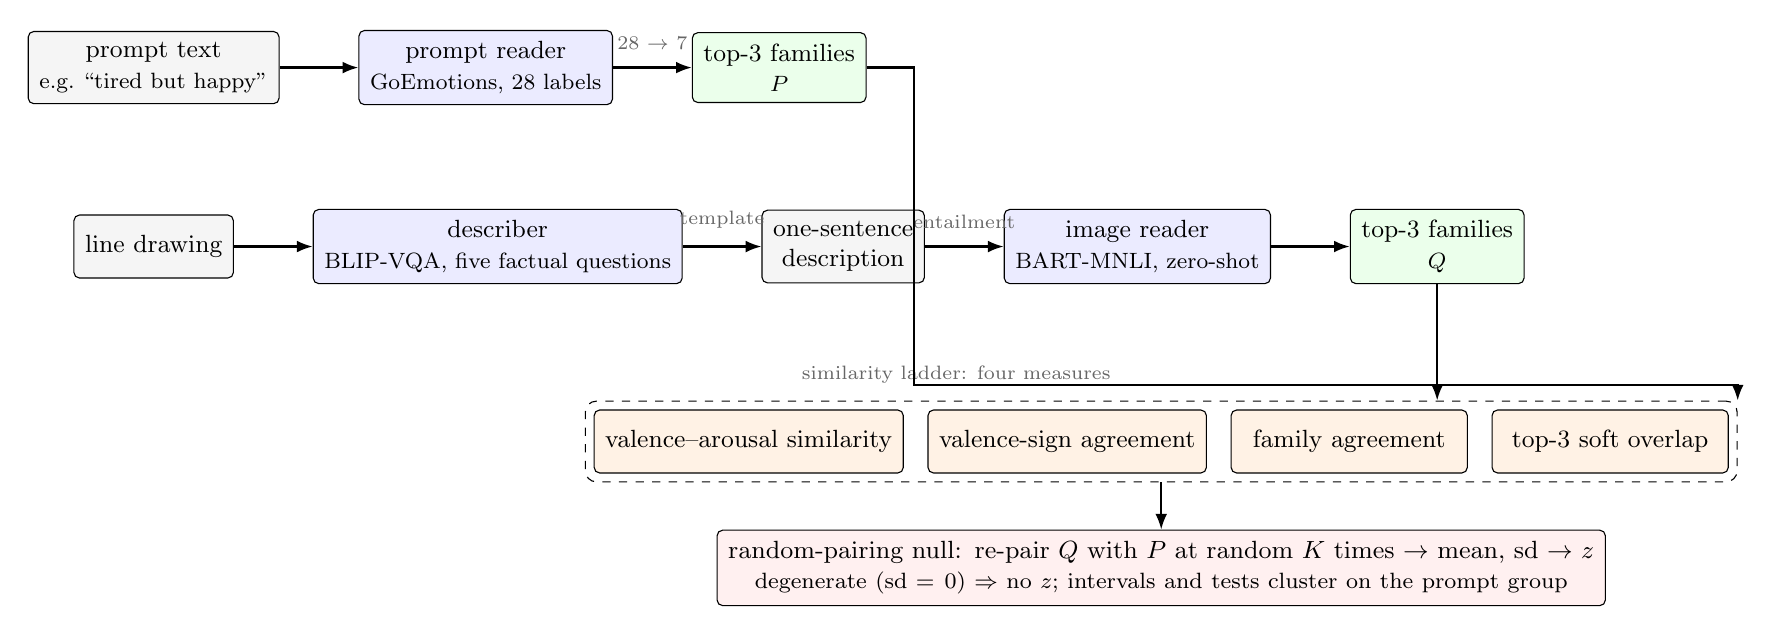
\begin{tikzpicture}[
  font=\small,
  node distance=6mm and 10mm,
  box/.style={draw, rounded corners=2pt, align=center, minimum height=8mm, inner sep=4pt, fill=white},
  data/.style={box, fill=black!4},
  model/.style={box, fill=blue!8},
  res/.style={box, fill=green!8},
  meas/.style={box, fill=orange!10, minimum width=30mm},
  arr/.style={-{Latex[length=2mm]}, thick},
  lab/.style={font=\scriptsize, text=black!60, yshift=1mm}
]
% prompt lane
\node[data] (prompt) {prompt text\\\footnotesize e.g.\ ``tired but happy''};
\node[model, right=of prompt] (goe) {prompt reader\\\footnotesize GoEmotions, 28 labels};
\node[res, right=of goe] (pfam) {top-3 families\\\footnotesize $P$};
\draw[arr] (prompt) -- (goe);
\draw[arr] (goe) -- node[lab, above] {28 $\to$ 7} (pfam);

% image lane
\node[data, below=14mm of prompt] (img) {line drawing};
\node[model, right=of img] (vqa) {describer\\\footnotesize BLIP-VQA, five factual questions};
\node[data, right=of vqa] (desc) {one-sentence\\description};
\node[model, right=of desc] (nli) {image reader\\\footnotesize BART-MNLI, zero-shot};
\node[res, right=of nli] (ifam) {top-3 families\\\footnotesize $Q$};
\draw[arr] (img) -- (vqa);
\draw[arr] (vqa) -- node[lab, above] {template} (desc);
\draw[arr] (desc) -- node[lab, above] {entailment} (nli);
\draw[arr] (nli) -- (ifam);

% ladder
\node[meas, below=16mm of desc, xshift=-12mm] (va) {valence--arousal similarity};
\node[meas, right=3mm of va] (sign) {valence-sign agreement};
\node[meas, right=3mm of sign] (fam) {family agreement};
\node[meas, right=3mm of fam] (ovl) {top-3 soft overlap};
\node[draw, dashed, rounded corners, inner sep=3pt, fit=(va)(sign)(fam)(ovl), label={[lab]above left:similarity ladder: four measures}] (ladder) {};
\draw[arr] (pfam.east) -- ++(6mm,0) |- ($(ladder.north east)+(0,2mm)$) -- (ladder.north east);
\draw[arr] (ifam.south) -- (ladder.north -| ifam.south);

% null
\node[box, fill=red!6, below=6mm of ladder, text width=110mm] (null) {random-pairing null: re-pair $Q$ with $P$ at random $K$ times $\to$ mean, sd $\to$ $z$\\\footnotesize degenerate (sd $=0$) $\Rightarrow$ no $z$; intervals and tests cluster on the prompt group};
\draw[arr] (ladder) -- (null);
\end{tikzpicture}
}
\caption{The chain from prompt and drawing to the four measures. Top: the prompt reader turns the visitor's words into three scored families. Middle: the describer answers five questions, the template makes one sentence of the answers, and the image reader scores the seven families by entailment. Bottom: the four measures and the random-pairing null that each of them is compared with; a null with zero spread yields no $z$, and every interval and test clusters on the prompt group.}
\label{fig:pipeline}
\end{figure}

\section{The corpus}
\label{sec:method-corpus}

The data are \nTotal{} records from Sheffield's Festival of the Mind in September 2024. Visitors typed how they felt. The box accepted any text, and each entry produced one drawing for the visitor to look at. Every drawing is monochrome line art, 1024 by 1024 pixels, because the installation software added a style instruction to every prompt, and the instruction itself was not passed on with the data. What arrived was one JSON file of \nTotal{} bare strings keyed by position, no labels, no metadata, no participant identifiers, plus a folder of \nTotal{} PNG files whose only link to the strings is their order.

Each PNG also carries a C2PA (Coalition for Content Provenance and Authenticity) provenance manifest. It names DALL$\cdot$E as the software agent, without a version, and holds no seed and no copy of the rewritten prompt that DALL$\cdot$E composes before it draws \cite{betker2023improving}, so nothing can be regenerated and the generation settings are unknown. Its signing time, though, did a lot of work in the pre-processing (Section~\ref{sec:method-preprocessing}).

Most prompts are short. Half of them have four words or fewer, the mean is about six, the longest runs to 107 words, and 294 of the analysed prompts consist of one word (Figure~\ref{fig:promptlength}). About 78\% never use a capital letter, and a handful are written in Italian, in French or in German. The commonest entry is ``happy'', drawn \nHappy{} times. Mixed feelings are common (``tired proud happy'', ``tired but happy''), and a fair number of entries are not about feelings at all: objects (``pigs''), pop culture (``mickey mouse''), questions put to the machine, place names.

Records are not people. Among the \nAnalysed{} analysed records, \nRepeats{} are repeats of a prompt someone had already typed, so how many people took part is unknown, \nDistinct{} is the upper bound, and any interval that treats records as independent will be too narrow (Section~\ref{sec:method-inference}). Figure~\ref{fig:dataset} gives the make-up of the corpus after pre-processing: \nPretest{} tests set aside, then the prompt reader's split (\nEmotional{} emotional, \nNonEmotional{} neutral-labelled) and, within the emotional prompts, the describer's (\nFaceEmo{} face-classified, \nSceneEmo{} scene-classified).

\begin{figure}[htbp]
\centering
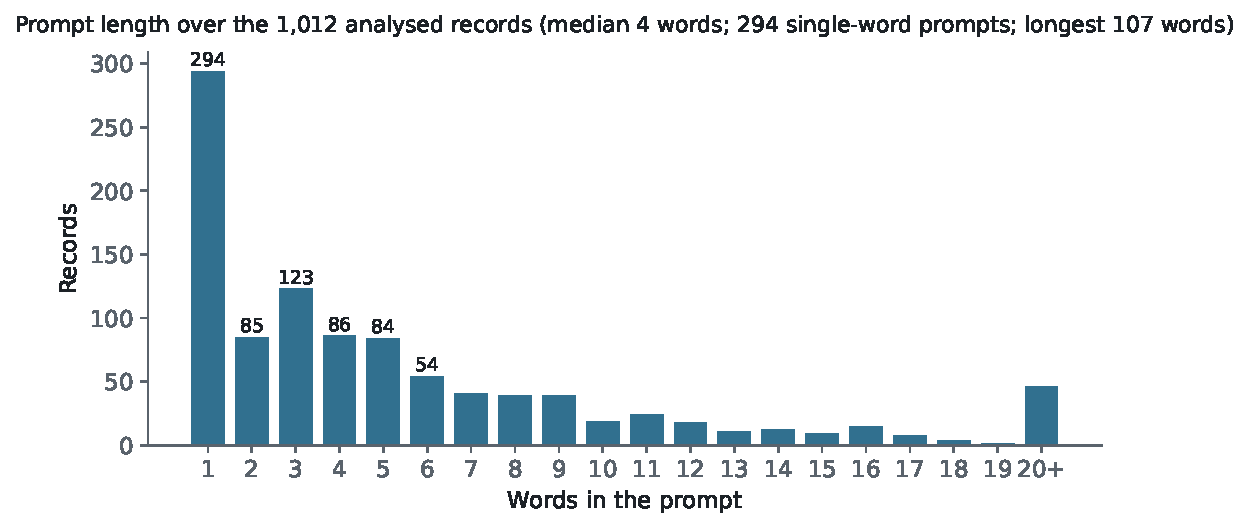
\includegraphics[width=\textwidth]{fig_prompt_length}
\caption{Word counts of the \nAnalysed{} analysed prompts, with the tail collapsed at twenty words: median four words, 294 prompts of one word, longest 107 words.}
\label{fig:promptlength}
\end{figure}

\begin{figure}[htbp]
\centering
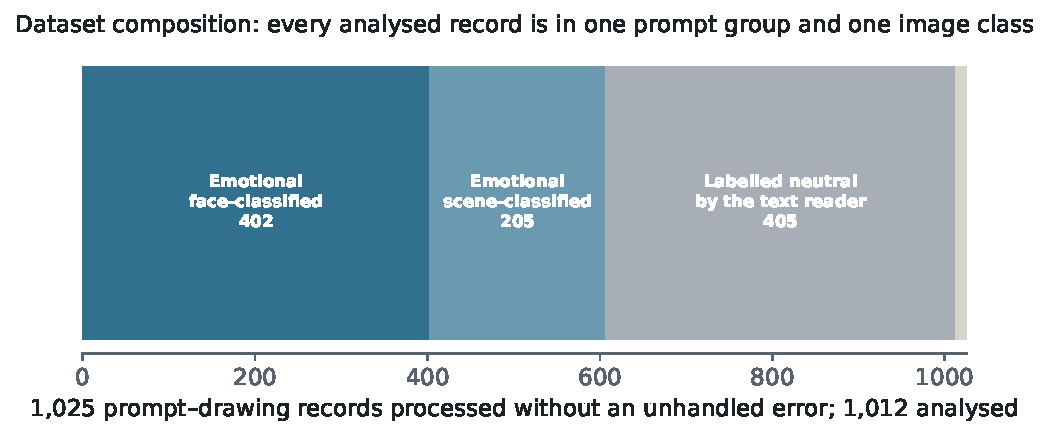
\includegraphics[width=\textwidth]{fig5_dataset}
\caption{What the \nTotal{} records became after pre-processing: \nPretest{} pre-festival tests set aside, then the \nAnalysed{} analysed records divided by the prompt reader into emotional and neutral-labelled prompts and, within the emotional prompts, by the describer into face-classified drawings and scene-classified ones. These are groupings for analysis; no analysed record is excluded by them.}
\label{fig:dataset}
\end{figure}


\section{Data pre-processing}
\label{sec:method-preprocessing}

\subsection{Loading and pre-test removal}

Nothing could be analysed until the files could be opened. Three naming patterns share one directory. The earliest records are zero-padded (\texttt{img\_00001.PNG}), the middle block is unpadded (\texttt{img\_200.PNG}), the records from 1000 onwards have a \texttt{t} before the number (\texttt{img\_t1000.PNG}), and records 2 and 4 end in lower-case \texttt{.png}, which a case-sensitive file system reads as another name. A loader written for the first pattern finds fewer than one file in five. \texttt{emoviz/data.py} handles all three and asserts that exactly \nTotal{} records resolve, so a missing file stops the run instead of quietly shrinking the sample.

The timestamps came out of the same loader. Every C2PA manifest carries an RFC-3161 signing time, and reading it gave each image a date the supplied files did not expose (Figure~\ref{fig:timeline}). The first \nPretest{} records date from 26 August to 18 September 2024, before the festival opened, on scattered days, as a developer testing the installation would, so they are excluded from every analysis and pushed through the pipeline all the same, so that the completion count covers everything. All the others up to the penultimate record fall on 19--29 September 2024, with none on 23 September. The last record, signed on 20 October 2024, is kept.

\begin{figure}[htbp]
\centering
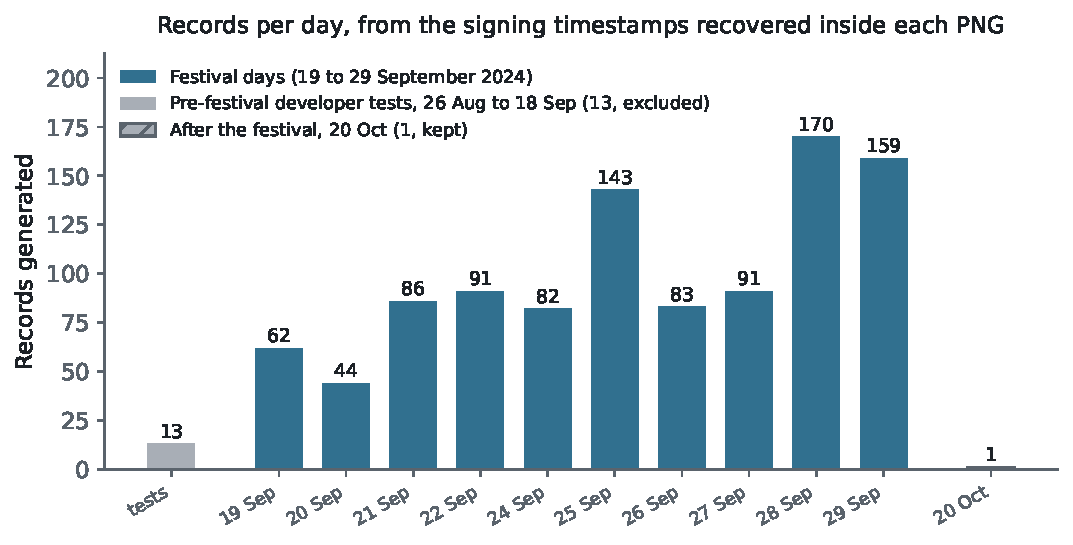
\includegraphics[width=\textwidth]{fig_timeline}
\caption{Records per day from the signing timestamps inside the PNG files. The \nPretest{} developer tests from 26 August to 18 September 2024 are shown apart on the left; the festival days run from 19 to 29 September with none on 23 September; the single record signed on 20 October is on the right and is kept.}
\label{fig:timeline}
\end{figure}

\subsection{Prompt groups}

Each record belongs to one prompt group. The group identifier is the prompt with surrounding whitespace removed and case folded. There are \nDistinct{} groups. \nGroups{} contain more than one record, those hold \nGroupRecords{} records, and \nPairGroups{} are pairs. The identifier is computed from the text as typed, before any name is redacted, and that order matters, because two different names collapse to one placeholder and an identifier computed after redaction would merge two unrelated prompts (this went wrong once in development, and the accounting test caught it). The identifier ignores case but the prompt reader did not, so a few groups hold two slightly different readings (``Ok'' and ``ok'' share one); no count changes because of it.

\subsection{Name redaction}

Eight prompts name a private individual, a friend, a relative, a teacher. Dr Chen's direction at the end of July was to handle this as data pre-processing, replacing the name of a private person with a placeholder while leaving in what visitors wrote about illness, grief and hard times, since that content identifies nobody on its own and the analysis needs it. Redaction runs at load time. The files on disk stay as they were, and analysis, figures and demonstrator all read the same redacted text.

The procedure has three stages, each written up in Appendix~\ref{app:instruments}. Detection favours recall. Since so few visitors used capitals, three detectors run together, an NLTK list of 7,944 given names \cite{bird2009natural}, capitalised tokens in mid-sentence that are missing from an English word list of 236,000 entries, and phrases of the form ``called X'' or ``my friend X''. Review attaches a decision, keep or redact, and a reason to every candidate and ties each redaction to one record, so that ``Jack Frost'' and ``woolly mammoth'' stay as they are. The audit refuses to pass while any candidate is undecided or any redaction entry has nothing left to act on. Application then swaps the token and merges adjacent placeholders.

Running the prompt reader again on the redacted text moved every family probability by 0.012 or less and left every top-1 family where it was, so every analysis uses the same prompt labels with or without the placeholder. Two entries were nothing but a name. They reduce to the bare placeholder (\CtrlNameOnly{} records), and the control audit (Section~\ref{sec:method-analyses}) confirms that they make no difference there either. The decision table names the tokens it removes, so it is kept with the dataset and out of the code folder.

\section{The pipeline}
\label{sec:method-pipeline}

\subsection{Prompt reader}

The prompt reader is RoBERTa fine-tuned on GoEmotions \cite{demszky2020goemotions}, the \texttt{SamLowe/\allowbreak roberta-base-go\_emotions} checkpoint, roughly 125 million parameters. Its output is 28 probabilities, one per category. These are added up into the seven families the GoEmotions authors proposed (Appendix~\ref{app:instruments}), the seven sums are rescaled so that they add to one, and the top three are kept as the prompt reading. A prompt counts as emotional whenever its top family is anything other than neutral, which makes \nEmotional{} of the \nAnalysed{} analysed prompts emotional and \nNonEmotional{} neutral-labelled. Nobody checked those labels. They are the reader's opinion, so the neutral-labelled prompts are kept as a group of their own and audited (Section~\ref{sec:method-analyses}).

GoEmotions was the third reader tried on this side. My first pipeline used a hand-built lexicon, transparent but unable to represent ``calm but tired'' except by letting one word win, and the prompts are full of blends like that. The same NLI model was then put on both sides. On short prompts it over-read surprise. Roughly a third of the corpus was labelled surprise in that run, the hypothesis wording misfiring on two-word inputs. GoEmotions has no such artefact. It was trained on Reddit comments written in the first person, as close to a festival entry as training data gets, and swapping it in left every headline result where it was.

\subsection{Describer}

The describer is BLIP-VQA \cite{li2022blip}, the \texttt{Salesforce/blip-vqa-base} checkpoint, roughly 385 million parameters. It gets five fixed questions per drawing. They always come in the same order, expression first, then action, posture, people count and scene (Appendix~\ref{app:instruments}), and none of the five contains the word ``emotion'', in keeping with the third principle above. The answers are cached record by record, so the template ablation can later repeat the extraction stage without touching the vision model at all.

BLIP-VQA is what remained after three attempts that went nowhere. The intended describer was Qwen2.5-VL, a vision--language model of 3 billion parameters, and on the 16~GB laptop available it filled the memory, swapped for 4~h~45~min and completed nothing. Florence-2 came next. It failed on the pinned Transformers 5.14 over a \texttt{forced\_bos\_token\_id} incompatibility. The plain captioning head of BLIP was tried next, but its captions were so terse that the image reader put almost every drawing into one family, surprise. With BLIP-VQA the full run over the \nTotal{} images completed, at between roughly 1 and 12 seconds a record, slowing when memory was short.

\subsection{Description template and image reader}

The five answers become one sentence. The template puts the people count and the scene first, ``A drawing of \{people\} showing \{scene\}.'', then the action and the posture, ``The person is \{action\}, \{posture\}.'', and last of all ``The facial expression is \{expression\}.'' (Appendix~\ref{app:instruments}). That sentence goes to BART fine-tuned on MultiNLI \cite{lewis2020bart, williams2018broad}, the \texttt{facebook/bart-large-mnli} checkpoint, roughly 407 million parameters, which scores, for each family, the hypothesis string ``This scene conveys \{family\}'' by entailment in the zero-shot manner of Yin and colleagues \cite{yin2019benchmarking}. The three best-scoring families form the image reading.

One property of the template matters later. The template states, for every record, that there is a person and that the person has a facial expression, even where the describer's own answer to the people question was zero, so a mountain reaches the reader with a person and a facial expression attached. It was written in week one. Nobody measured what that did until the audits in September (Sections~\ref{sec:results-describer} and \ref{sec:results-ablation}). GoEmotions, the one other reader tried on this side, put almost everything in neutral with nearly all the probability on that family, because it wants feeling words in the first person, which a description of a drawing never has.

\subsection{Face and scene classes}

Dr Chen expected faces to be easier than scenes for any reader and asked for the split. The rule is mechanical. Face-classified means two things are true of the describer's answers, that the people count is at least one and that the expression answer contains, as a whole token, one of the readable expression words in Appendix~\ref{app:instruments}, so ``man is smiling'' qualifies. Everything else is scene-classified. A digit or a number word in the people answer gives the count. Over all \nAnalysed{} analysed records the split is \nFaceAll{} to \nSceneAll{}, and inside the emotional prompts it is \nFaceEmo{} to \nSceneEmo{}. The rule was tightened on 1 September, after the first audit, so that only whole tokens count.

The split is partly circular. The class comes out of the describer's answers, and the image reader reads a sentence built from those same answers, which makes part of the face/scene contrast a contrast between two kinds of description. Chapter~\ref{ch:results} puts a number on it. The single-coder check, where a sample of drawings is classed by a person who has not seen the describer's answers, is the only place it is broken.

\section{The similarity ladder}
\label{sec:method-measures}

Each reader returns three families with scores, $T = \{(\ell_i, s_i)\}_{i=1}^{3}$ with $\ell_i \in \mathcal{F}$ and $\mathcal{F} = \{\text{joy}, \text{sadness}, \text{anger}, \text{fear}, \text{surprise}, \text{disgust}, \text{neutral}\}$. $P$ is the prompt reader's list, $Q$ the image reader's; $\operatorname{top}(T) = \ell_1$ is the top family. Each family also has $c_\ell = (v_\ell, a_\ell)$, a fixed point on the valence--arousal plane (Appendix~\ref{app:instruments}). They were placed by hand from the usual positions of the basic emotions on Russell's circumplex \cite{russell1980circumplex}; per-family averages of the NRC valence and arousal norms \cite{mohammad2018obtaining} are the documented alternative, left for further work. The four measures are defined below, beginning with the loosest.

\paragraph{Valence--arousal similarity.} A reading is first reduced to one point on the plane, its score-weighted centroid, and two readings are compared by the distance between their points:
\begin{equation}
\mathbf{v}(T) = \frac{\sum_i s_i\, c_{\ell_i}}{\sum_i s_i}, \qquad
S_{\mathrm{VA}}(P, Q) = 1 - \frac{1}{\sqrt{2}}\,\Bigl\|\Bigl(\tfrac{v_P + 1}{2} - \tfrac{v_Q + 1}{2},\; a_P - a_Q\Bigr)\Bigr\|_2 ,
\label{eq:va}
\end{equation}
Here $(v_P, a_P)$ is $\mathbf{v}(P)$, likewise for $Q$, and valence is mapped onto $[0,1]$ so the two axes span the same range. This rung forgives. A prompt read as joy against a drawing read as surprise scores well here, since the two points lie near each other, although the top families differ. The minimum over the seven fixed points is $0.412$ (joy paired with sadness), and random pairings already average about \FullNeuVaNull{}, so this measure is never reported without its null beside it.

\paragraph{Top-3 soft overlap.} The two readers score on different scales, so each side is rescaled so that its three scores sum to one, $\tilde{p}_\ell = s_\ell / \sum_j s_j$, and the overlap adds up, family by family, the smaller of the two shares,
\begin{equation}
S_{\mathrm{ovl}}(P, Q) = \sum_{\ell \in \mathcal{F}} \min\bigl(\tilde{p}_\ell,\; \tilde{q}_\ell\bigr) \in [0, 1],
\label{eq:overlap}
\end{equation}
It equals one exactly when the two sides coincide. Credit goes to a second or third family that both readers listed, which the top rung ignores, and of the four rungs this is the only one that uses the scores as well as the labels.

\paragraph{Family agreement.} For $n$ records the rate is
\begin{equation}
A_{\mathrm{fam}} = \frac{1}{n} \sum_{i=1}^{n} \mathbb{1}\bigl[\operatorname{top}(P_i) = \operatorname{top}(Q_i)\bigr].
\label{eq:family}
\end{equation}
Of the four this is the least forgiving, and it is the one other studies most often report. Its chance level depends on the marginals. A reader that answers joy for many drawings will agree by accident with a prompt reader that answers joy for many prompts, and Table~\ref{tab:families} shows that both readers here do exactly that.

\paragraph{Valence-sign agreement.} Let $\sigma(\ell) \in \{+, -, 0\}$ map joy to $+$, surprise and neutral to $0$, and the other four families to $-$. Then
\begin{equation}
A_{\mathrm{sign}} = \frac{\sum_{i} \mathbb{1}\bigl[\sigma(\operatorname{top} P_i) \neq 0 \;\wedge\; \sigma(\operatorname{top} P_i) = \sigma(\operatorname{top} Q_i)\bigr]}{\sum_{i} \mathbb{1}\bigl[\sigma(\operatorname{top} P_i) \neq 0\bigr]} ,
\label{eq:sign}
\end{equation}
so a record with an unsigned prompt family drops out of the denominator, and the denominator is printed beside every value it produces; for the emotional prompts it is \FullEmoNSign{} of \FullEmoN{}. It asks the coarsest question there is, whether both readers gave the same sign, and the headline result rests on it.

\section{The random-pairing null}
\label{sec:method-null}

None of the measures starts at zero. Equation~\ref{eq:va} is bounded below, and both readers say joy so often (Table~\ref{tab:families}) that top-1 agreement happens by accident. So every value is compared with the same measure after the image readings have been shuffled against the prompts, the exchangeability hypothesis \cite{good2005permutation}: if a drawing's reading has nothing to do with its prompt, handing each prompt somebody else's drawing changes the measure only by noise. For any subset of $n$ records and any measure $m$, the image side is permuted $K$ times, $\pi_k$ being the $k$-th permutation, and $m_k$ is the measure recomputed on the pairs $(P_i, Q_{\pi_k(i)})$; with $\hat\mu = \frac{1}{K}\sum_k m_k$ the mean of these values and $\hat\sigma$ their standard deviation,
\begin{equation}
z = \frac{m_{\mathrm{obs}} - \hat\mu}{\hat\sigma}, \qquad K = \nullShuffles,\ \text{seed}\ \nullSeed .
\label{eq:z}
\end{equation}

There are two cautions on $z$. First, \nullShuffles{} re-pairings give a rough estimate of the standard deviation in the denominator. Re-running with seeds 1 to 5 puts the headline valence-sign $z$ anywhere from \ZSeedMin{} to \ZSeedMax{} (the null mean moves by under a tenth of a point). $z$ is therefore used to rank effects and never as an exact probability. Second, a null can be degenerate. When a subset's prompts all have the same top family, shuffling the drawings leaves family agreement exactly where it was, and likewise for the sign when every prompt has the same sign; $\hat\sigma$ comes out at zero and $z$ is undefined. The scripts spot this from the spread of the null itself and print nothing in that cell. Before that, two subsets had been flagged by hand and a third missed.

\section{Inference}
\label{sec:method-inference}

Records are not independent, and for a while they were analysed as if they were. \nRepeats{} records share their prompt with an earlier one, and all the drawings of one prompt inherit whatever that prompt does to each reader. The face/scene permutation test and the interval on that difference were run just before the presentation on 4 September; everything else here, the clustered intervals for every other cell, Cohen's kappa, the Holm correction and the paired tests for the two image readers, was added in the second audit on 9 September, when the marking criteria were revisited. The unit of resampling throughout is the prompt group \cite{cameron2008bootstrap}.

\paragraph{Clustered bootstrap intervals.} Let $\mathcal{G}$ be the prompt groups in a subset. One draw takes $|\mathcal{G}|$ groups with replacement, pools every record of the groups it drew and recomputes the measure, and the interval is the middle 95\% of the $B$ bootstrap values \cite{efron1993introduction}, $B = \DiffDraws{}$, seed \nullSeed{}. A group drawn twice counts twice, so a prompt drawn \nHappy{} times moves the interval as one piece of evidence and never as \nHappy{}.

\paragraph{Clustered permutation test of the face/scene difference.} Under the null the image class has no bearing on agreement, so face/scene labels can be shuffled over prompt groups. That is done $P$ times, recomputing the difference each time and counting how often the shuffled difference is at least as extreme as the real one; the two-sided $p$-value follows North and colleagues \cite{north2002note},
\begin{equation}
p = \frac{k + 1}{P + 1}, \qquad k = \#\{\text{permuted differences at least as extreme as the observed}\},
\label{eq:permp}
\end{equation}
With $P = \DiffDraws$ the smallest value that can come out is $10^{-4}$.

\paragraph{Cohen's kappa.} Family agreement is also given as Cohen's kappa, for comparison with other studies,
\begin{equation}
\kappa = \frac{p_o - p_e}{1 - p_e},
\label{eq:kappa}
\end{equation}
Here $p_o$ is the top-1 rate actually observed and $p_e$ the rate the two readers' family marginals would produce on their own if the readers had nothing to do with each other \cite{cohen1960coefficient}. Landis and Koch's bands \cite{landis1977measurement} give the words for it. The interval is the same clustered bootstrap.

\paragraph{Multiple comparisons.} \HolmM{} $z$-scores survive the degeneracy filter. Each becomes a two-sided $p$-value under the normal approximation, and Holm's step-down procedure \cite{holm1979simple} controls the family-wise rate: with the $p$-values sorted, $p_{(1)} \le \dots \le p_{(m)}$, rejection proceeds in order and stops at the first $p_{(i)} > \alpha / (m - i + 1)$, at $\alpha = 0.05$. For the largest $z$ the normal approximation is only nominal, and no decision changes because of it.

\paragraph{Paired comparison of two image readers.} Each record gives each reader a yes or a no. The comparison is therefore paired. Let $b$ be the number of records where only the first reader agrees and $c$ the number where only the second does. McNemar's exact test \cite{mcnemar1947note} on $(b, c)$ assumes independent records and is therefore optimistic here, so a clustered alternative sums the differences inside each prompt group and flips the sign of whole groups at random, \McClusterDraws{} times; the interval on the rate difference is again a clustered bootstrap.

\paragraph{Wilson intervals.} The single-coder check produces proportions from a small sample, some of them near 0 or 1, so they get Wilson score intervals \cite{wilson1927probable}, which behave where the normal interval breaks down.

\section{Analyses}
\label{sec:method-analyses}

The list below follows the order of Chapter~\ref{ch:results}. Each analysis is one script writing one JSON file, and every table, figure and number in the text is generated from those files (Appendix~\ref{app:repro}).

\paragraph{Splits and the main table.} \texttt{analysis\_final.py} produces the main table, four measures each with its null, for the emotional prompts, for the face-classified and the scene-classified records inside them, for the positive and the negative prompts, and for the neutral-labelled prompts, all by Equation~\ref{eq:z}. Only valence--arousal similarity has a live null in the single-valence cells. The same script repeats the table on distinct prompts only, keeping the first record of each of the \nDistinct{} groups, and that is the robustness check for repeated prompts.

\paragraph{The face/scene difference.} \texttt{significance.py} runs the permutation test and the bootstrap interval for the difference, for valence sign and for family. Then \texttt{inference.py} supplies the intervals for the remaining cells, kappa for the emotional, face and scene cells, the Holm step-down over the printed $z$-scores, and the seed check.

\paragraph{Specificity check.} Neutral-labelled prompts are the specificity check: their agreement should sit at the null. Only valence--arousal similarity can be read there, since on a subset with one prompt label the other three nulls have no spread, and the analysis reports the degeneracy in place of a $z$.

\paragraph{Method comparison.} \texttt{method\_comparison.py} changes the image reader and nothing else, with an identical prompt reader, identical records (\McN{} of them), identical measures and identical re-pairings. The second reader is direct CLIP \cite{radford2021learning, ilharco2021openclip}. It is OpenCLIP ViT-B/32 with LAION-2B weights, given the seven family names as text prompts, and its readings sit frozen in a file the main pipeline cannot overwrite. A first-build comparison had used NLI on the prompt side, another subset and another overlap formula, and the first audit on 1 September found its direct-CLIP overlap computed over the wrong label space. Table~\ref{tab:methodvone} keeps it as a record only; the like-for-like version dates from 9 September.

\paragraph{Consistency across repeated prompts.} For a repeat group $g$ of $n_g \ge 2$ records, write $c_g = \max_{\ell} n_{g,\ell} / n_g$ for the share of its drawings given the group's commonest image family. The consistency $C$ is the mean of $c_g$ over the \nGroups{} groups. A pair cannot score under $0.5$, and \nPairGroups{} groups are pairs, so the null shuffles image families over all \nAnalysed{} analysed records, keeps the group boundaries where they are and recomputes $C$, \ConsDraws{} times, and the number of groups with $c_g = 1$ gets the same treatment. The scripted null is a 9 September addition. $C$ bounds the reproducibility of prompt, generator and reader together; it cannot isolate the generator, whose settings were never recorded, and one visitor entering ``happy'' twice looks identical to two visitors entering it once each.

\paragraph{Per-family agreement.} \texttt{audits.py} also breaks family agreement down by prompt family, as the fraction of each prompt family's records that the image reader put in the same family, with clustered intervals; Table~\ref{tab:confusion} has the full cross-tabulation.

\paragraph{Control audit.} The same script scans the \CtrlN{} neutral-labelled prompts for any of \CtrlLexicon{} ordinary affect words, and it picks out the \CtrlNameOnly{} records that redaction reduced to the bare placeholder. The specificity check is then re-run without either set.

\paragraph{Describer audit and copy rate.} The describer's people count is tabulated against whether an expression word is present, and the smile answers are counted with their denominators. The copy rate concerns one-word expression answers. It is the fraction of those records on which the image reader's top family coincides with the family of that word; the strict version admits only words that name a feeling (happy, sad, angry and the like, \DescBareStrictN{} records) and the broad version adds facial actions such as smile and crying (\DescBareBroadN{} records).

\paragraph{Error taxonomy.} \texttt{error\_taxonomy.py} collects the emotional records on which the two readers disagree about the top family while each gives its own top family a score of at least 0.8. Fewer than the intended 40 qualified, so all were examined. An automatic tagger first marks each record (people count, bare expression word, short prompt, ambiguous raw label, connective), and then every drawing was opened and one primary failure mode chosen out of six fixed ones: (a) an invented face or expression, (b) a misread one, (c) a fair description the reader mis-inferred from, (d) a mixed or ambiguous prompt, (e) a drawing unrelated to its prompt, and (f) a prompt the prompt reader mislabelled. A fixed tie-break rule, printed with the counts, settled records where more than one applied.

\paragraph{Template ablation.} \texttt{ablate\_nli.py} takes the cached answers, builds each description again with a modified template, sends only that sentence back through the image reader, and then computes the ladder and the nulls exactly as the main analysis does, seed included. There are five single-clause deletions (expression, action, posture, people, scene), one variant that sets every expression to ``unclear'', and two people-aware variants that shorten the sentence for records with a zero people count, one keeping the action and posture clauses and one keeping only the scene clause. A control run with the original template separates numerical noise from real template effects. It changed \AblControlChanged{} top-1 readings.

\paragraph{Single-coder check.} \texttt{human\_check.py} draws the sample and scores the coding. The sample is 120 drawings chosen by seed in three strata defined by the describer's output, 40 from the face-classified records, 40 from scene-classified records with a zero people count, and every record whose people answer was vague or a single word, the remainder split equally between the first two strata. Six numbered contact sheets hold the drawings and nothing else. The author is the coder, filling the four columns in Appendix~\ref{app:instruments} blind to prompt, description and readings. Once coded, the script scores the people count and the precision and recall of the face rule, both against the coder, what lies behind the ``smiling'' answers, and the coder's valence against the image reader's, with Wilson intervals, and then recomputes the face/scene difference on the coder's classification, the one estimate free of the describer's split. The coding was not finished at the time of writing. Figure~\ref{fig:codingsheet} shows the first sheet.

\begin{figure}[htbp]
\centering
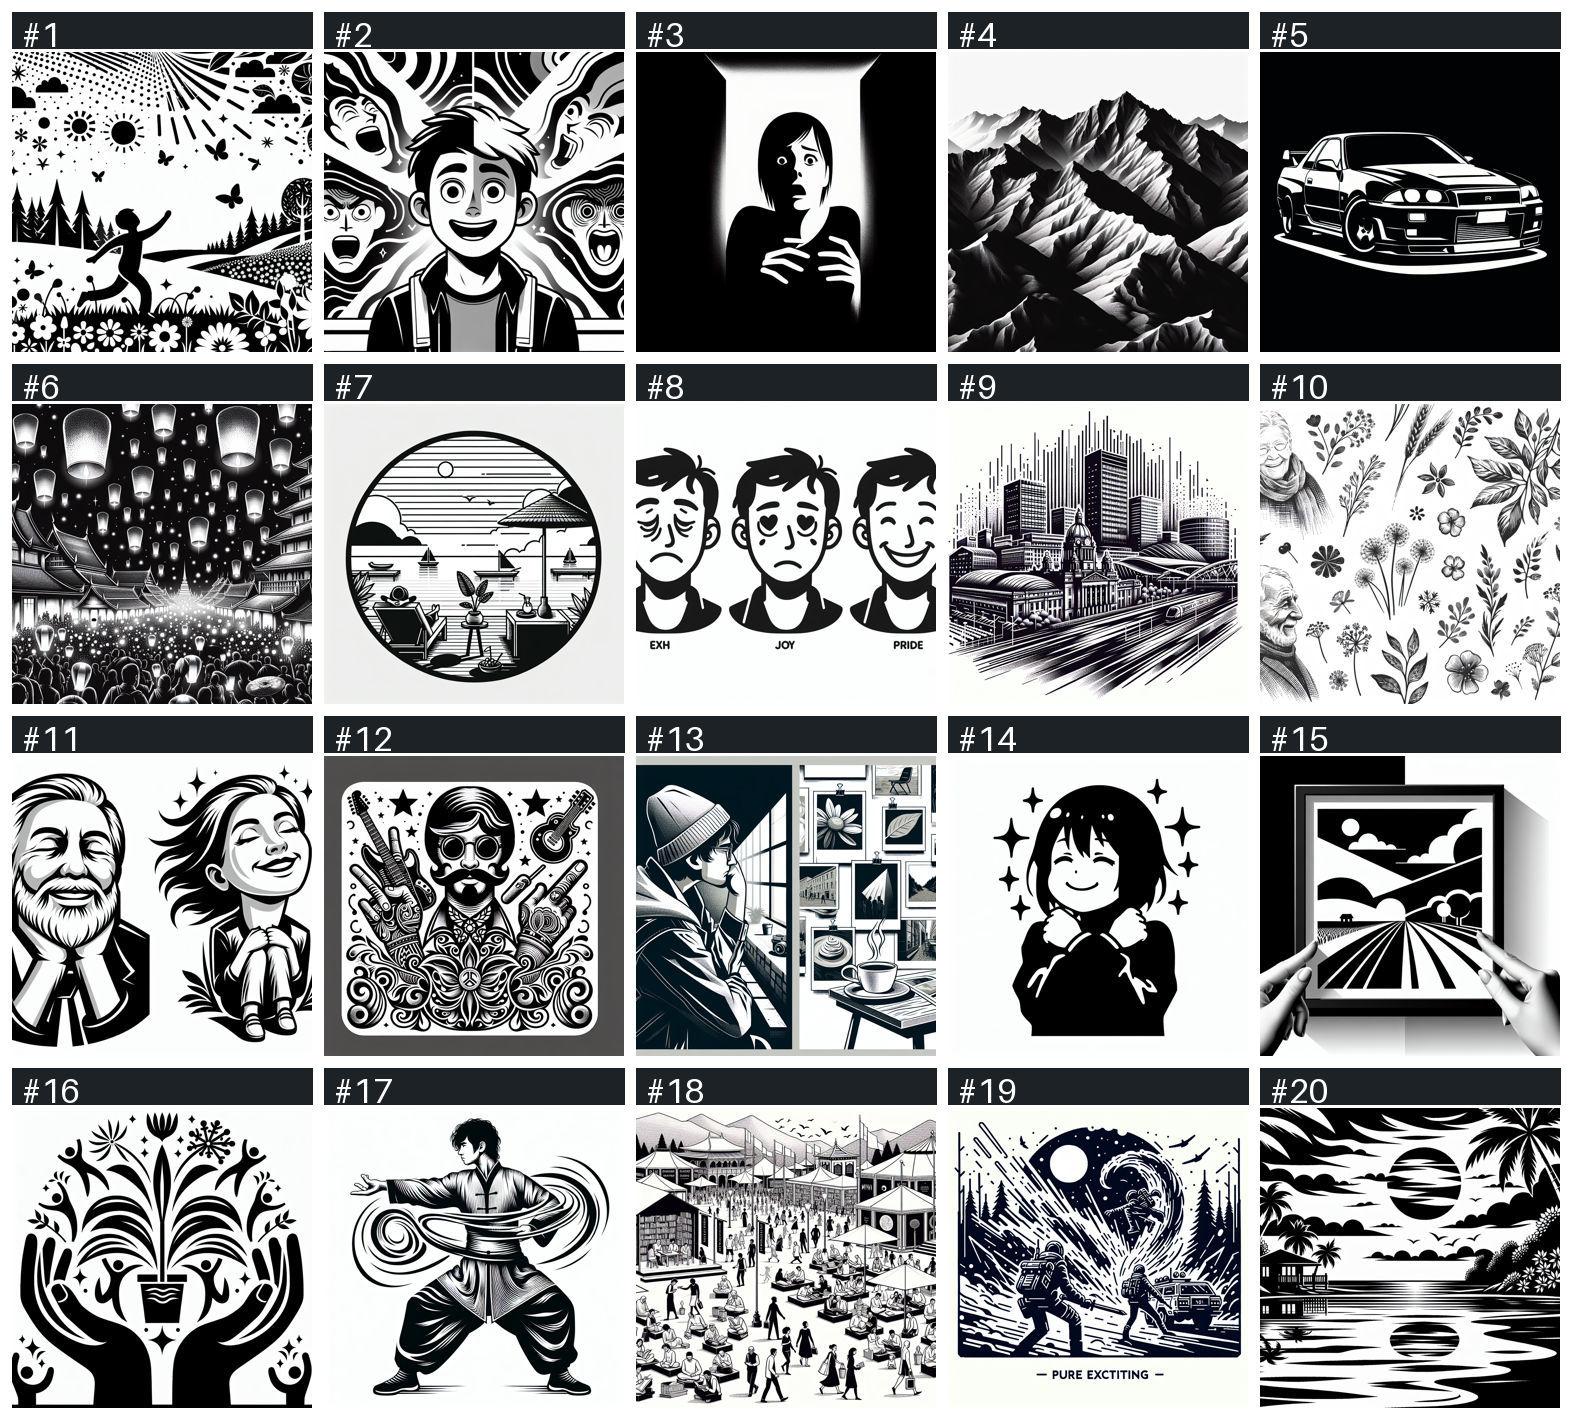
\includegraphics[width=0.9\textwidth]{coding_sheet}
\caption{The first of the six contact sheets for the single-coder check. Only the drawings and their sheet numbers are shown; the prompt, the description and both readings stay hidden until the coding file is complete.}
\label{fig:codingsheet}
\end{figure}

\section{The demonstrator}
\label{sec:method-demo}

The pipeline also runs as a local Flask application, \texttt{app.py} with one page in \texttt{web/index.html}, on port 5050. It applies the real models to any analysed record or an uploaded image and shows the five answers, the sentence built from them, both readings, and the four measures against the null the analysis used, computed when the server starts from the result files. Three choices in the interface come straight from the methodology. The axis for valence--arousal similarity begins at 0.412, its floor, and the middle half of the random pairings is shaded across it, so a below-chance value sits visibly under the band. The verdict puts valence sign and family first and gives the loosest measure only as a percentile among the random pairings. A degenerate chance level is named as degenerate, with no number. The page stores nothing that is typed or uploaded, the request log is switched off, and it was never used to collect data.

\begin{figure}[htbp]
\centering
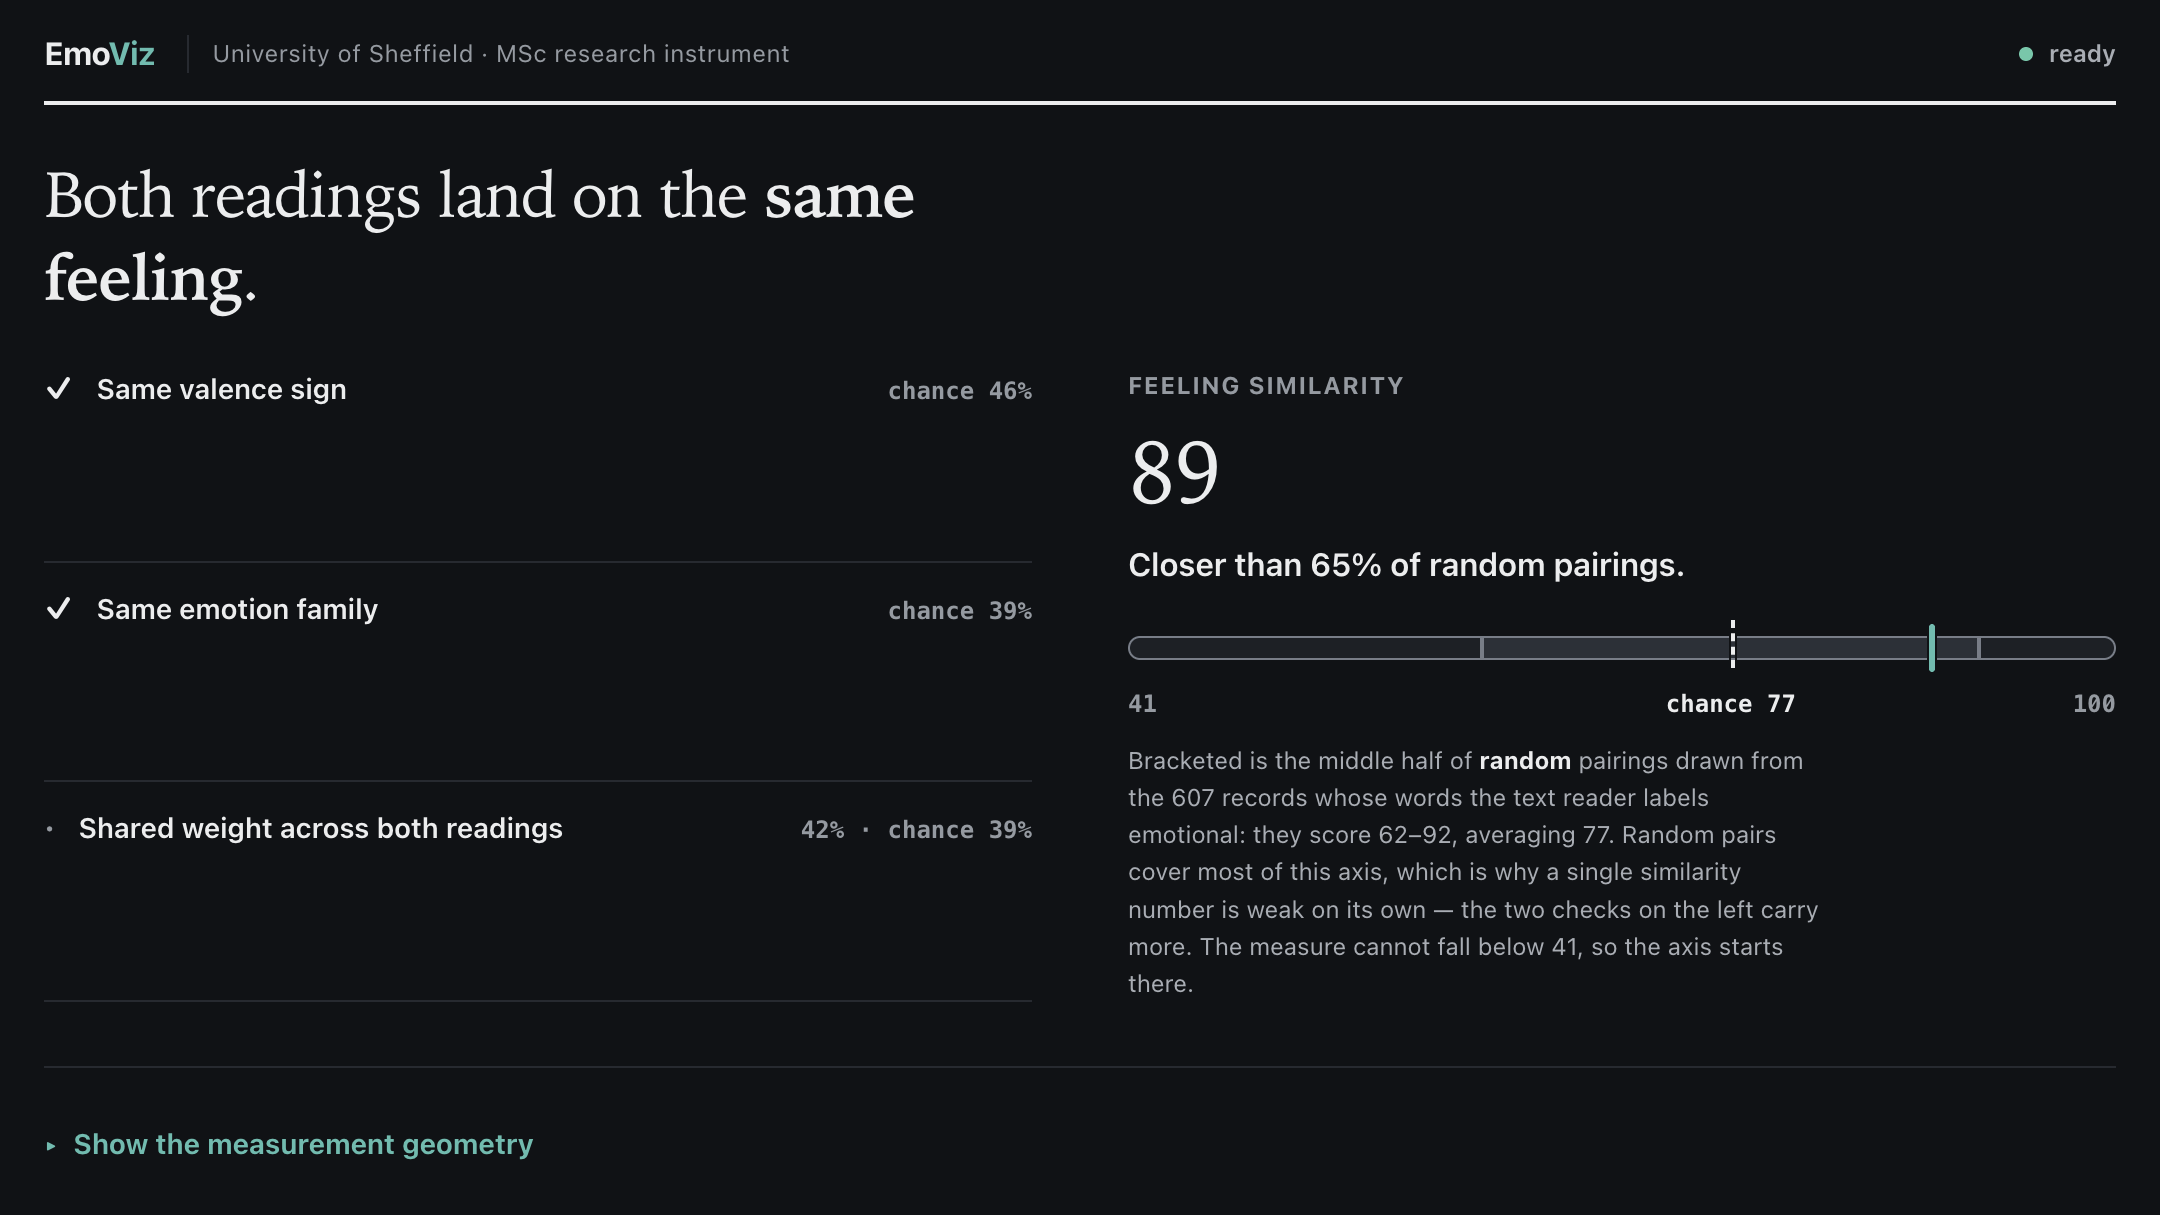
\includegraphics[width=\textwidth]{demo_screenshot}
\caption{The demonstrator's verdict after running record 63, ``super tired'', through the live models. Valence sign and family are reported first, each beside the chance level for that measure, and the third row gives the top-3 overlap. Valence--arousal similarity is not scored as a check but placed on its own axis on the right: the axis starts at its floor of 41, the shaded bracket is the middle half of the random pairings, the dashed mark is their mean and the solid mark is this record.}
\label{fig:demo}
\end{figure}

\section{Reproducibility and testing}
\label{sec:method-repro}

The environment is pinned in \texttt{requirements.txt}, Python 3.12 with PyTorch 2.13 and Transformers 5.14, on Apple silicon in float16, with about 3.5~GB of model downloads on first use. Every random process is seeded. Model outputs are cached record by record, the pipeline checkpoints to a JSONL file after each record so that a crash resumes where it stopped, and every stage after the pipeline reruns in seconds. Direct CLIP's readings are frozen in a file.

A single module, \texttt{emoviz/metrics.py}, defines each measure, each constant, the split rule and the null exactly once, and the scripts import from it, so a formula has nowhere to drift. Before it existed, two scripts had their own overlap formulas. They differed slightly. The difference changed no result on this data.

Testing has two layers. The first, \texttt{test.sh}, is a shell smoke suite: it verifies the environment, checks that the corpus and the cached outputs are intact, runs the redaction audit, runs each analysis script and requires a clean exit, pushes three fresh images through the live pipeline, and builds the figures, and any failure gives a non-zero exit. The second, \texttt{test\_numeric.py}, pins the headline numbers, comparing each one quoted in the text with the JSON value it comes from, to a stated tolerance, and it also unit-tests the measures themselves, the 0.412 floor, symmetry, overlap bounds and scale invariance, the sign map and the face rule. Figures come from \texttt{make\_figures.py} and the tables and macros from \texttt{export\_tex.py}, both reading the same JSON, so no result in this document was typed by hand.

The tests also have a limit. None of them compares a model's answer with a person's judgement. The completion figure, every one of the \nTotal{} images run through without an unhandled error, says that the code did not crash and nothing about whether its answers are any good, and a person enters the chain at one point only, the single-coder check. Appendix~\ref{app:repro} has the file list and the run order.
   % Methodology
\chapter{Results}
\label{ch:results}

This chapter reports the results in the order Section~\ref{sec:method-analyses} introduced the analyses. Interpretation is kept for Chapter~\ref{ch:discussion}. Every statistic in this chapter is taken from the analysis result files, and the tables are built from the same files. Each rate is set beside the random-pairing null for its own subset, built by re-pairing image readings and prompts at random \nullShuffles{} times under seed \nullSeed{}, and each interval is a 95\% clustered bootstrap over prompt groups with \DiffDraws{} draws.

\section{Overall agreement}
\label{sec:results-overall}

Table~\ref{tab:headline} is the main table. It holds the four measures for the \nEmotional{} emotional prompts, and Figure~\ref{fig:zgroup} plots each of those cells as a distance from its null, in units of the null's standard deviation. Every rung of the ladder sits above chance. On valence sign the rate is \FullEmoSignObs{} where random re-pairing gives \FullEmoSignNull{} ($z$ = \FullEmoSignZ{}, 95\% confidence interval (CI) \FullEmoSignCi{}). Its denominator is \FullEmoNSign{} of the \FullEmoN{}, because a prompt whose top family is surprise has no valence sign. Family agreement comes to \FullEmoFamObs{} against \FullEmoFamNull{} ($z$ = \FullEmoFamZ{}, CI \FullEmoFamCi{}) and top-3 soft overlap to \FullEmoOvlpObs{} against \FullEmoOvlpNull{} ($z$ = \FullEmoOvlpZ{}). Valence--arousal similarity is \FullEmoVaObs{} against \FullEmoVaNull{} ($z$ = \FullEmoVaZ{}). So the loosest measure gives the largest $z$ of the four, and the smallest gap in points between observed and null. Because of the floor in Equation~\ref{eq:va}, random pairs already score high on this measure and the null barely varies, so a few points above it come to many multiples of the null's spread.

% GENERATED by emoviz/export_tex.py — do not edit
\begin{table}[htbp]
\centering
\small
\caption{Agreement between the prompt reader and the image reader on the 1,012 analysed records, by prompt group and image class, against the random-pairing null (300 re-pairings, seed 7). CI: clustered bootstrap over prompt groups (10,000 draws). n/a: degenerate null (every prompt in the subset shares one label, so permutation cannot change the score).}
\label{tab:headline}
\begin{tabular}{lrrrl}
\toprule
Subset / measure & Observed & Null & $z$ & 95\% CI \\
\midrule
\textbf{Emotional prompts} ($n$=607; sign $n$=530) &  &  &  &  \\
Valence--arousal similarity & 83.8\% & 77.3\% & +12.2 & [82.0, 85.5] \\
Valence-sign agreement & 64.0\% & 45.6\% & +11.1 & [58.6, 68.8] \\
Family agreement & 53.0\% & 38.8\% & +10.3 & [47.3, 58.7] \\
Top-3 soft overlap & 50.6\% & 39.4\% & +11.6 & [46.5, 54.7] \\
\midrule
\textbf{\quad face-classified} ($n$=402; sign $n$=360) &  &  &  &  \\
Valence--arousal similarity & 84.2\% & 76.4\% & +11.2 & [82.3, 86.1] \\
Valence-sign agreement & 73.9\% & 53.5\% & +10.4 & [68.3, 79.2] \\
Family agreement & 61.9\% & 45.8\% & +10.3 & [55.8, 68.0] \\
Top-3 soft overlap & 53.4\% & 40.4\% & +11.6 & [49.2, 57.7] \\
\midrule
\textbf{\quad scene-classified} ($n$=205; sign $n$=170) &  &  &  &  \\
Valence--arousal similarity & 82.9\% & 79.1\% & +6.0 & [80.4, 85.2] \\
Valence-sign agreement & 42.9\% & 29.6\% & +5.8 & [33.1, 51.1] \\
Family agreement & 35.6\% & 26.2\% & +4.4 & [26.4, 44.1] \\
Top-3 soft overlap & 44.9\% & 38.1\% & +4.9 & [38.7, 51.0] \\
\midrule
\textbf{Neutral-labelled prompts} ($n$=405; sign $n$=0) &  &  &  &  \\
Valence--arousal similarity & 76.6\% & 76.6\% & +0.3 & [75.6, 77.6] \\
Valence-sign agreement & 0.0\% & 0.0\% & n/a & degenerate \\
Family agreement & 28.6\% & 28.6\% & n/a & degenerate \\
Top-3 soft overlap & 31.6\% & 31.6\% & +0.0 & -- \\
\bottomrule
\end{tabular}
\end{table}


\begin{figure}[htbp]
\centering
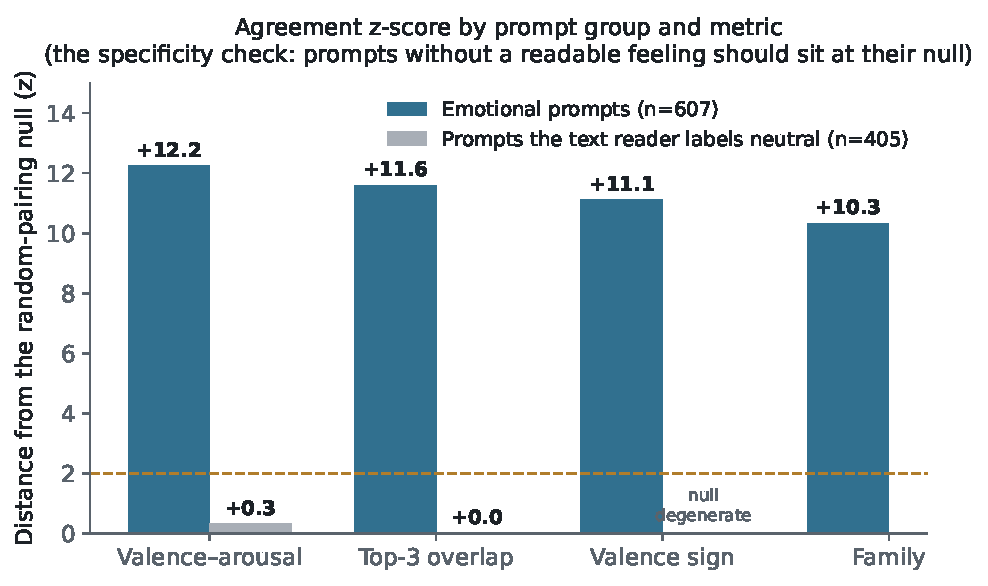
\includegraphics[width=0.9\textwidth]{fig3_z_by_prompt_group}
\caption{Distance from the random-pairing null, in standard deviations of that null ($z$), by prompt group and by measure. The neutral-labelled group has a degenerate null for valence sign and for family, so those two cells are left empty.}
\label{fig:zgroup}
\end{figure}

\section{Face-classified versus scene-classified drawings}
\label{sec:results-face-scene}

Figure~\ref{fig:facescene} and Table~\ref{tab:difference} divide the same \nEmotional{} prompts by the class the describer's answers assign to the drawing. Faces are the larger class, with \FullFaceN{} records. There valence-sign agreement reaches \FullFaceSignObs{} where the null is \FullFaceSignNull{} ($z$ = \FullFaceSignZ{}, CI \FullFaceSignCi{}), and family agreement reaches \FullFaceFamObs{} where the null is \FullFaceFamNull{} ($z$ = \FullFaceFamZ{}). The \FullSceneN{} scene-classified records come out lower on both rungs, at \FullSceneSignObs{} on valence sign (null \FullSceneSignNull{}, $z$ = \FullSceneSignZ{}, CI \FullSceneSignCi{}) and \FullSceneFamObs{} on family (null \FullSceneFamNull{}, $z$ = \FullSceneFamZ{}). In this table both classes clear their nulls. The scene row comes up again in Section~\ref{sec:results-ablation}.

Each class has a null of its own. For that reason the contrast is stated as a difference in percentage points and tested with the clustered permutation procedure from Section~\ref{sec:method-inference}, which gives face minus scene as \DiffSignPp{} for valence sign (clustered interval \DiffSignCi{}) and \DiffFamPp{} for family (interval \DiffFamCi{}). The permutation test returns $p$ = \DiffSignP{} for valence sign and $p$ = \DiffFamP{} for family, the smallest value it can report with the number of permutations run. Valence--arousal similarity hardly moves between the classes (\FullFaceVaObs{} for faces, \FullSceneVaObs{} for scenes), so the gap between them sits in the two categorical rungs.

\begin{figure}[htbp]
\centering
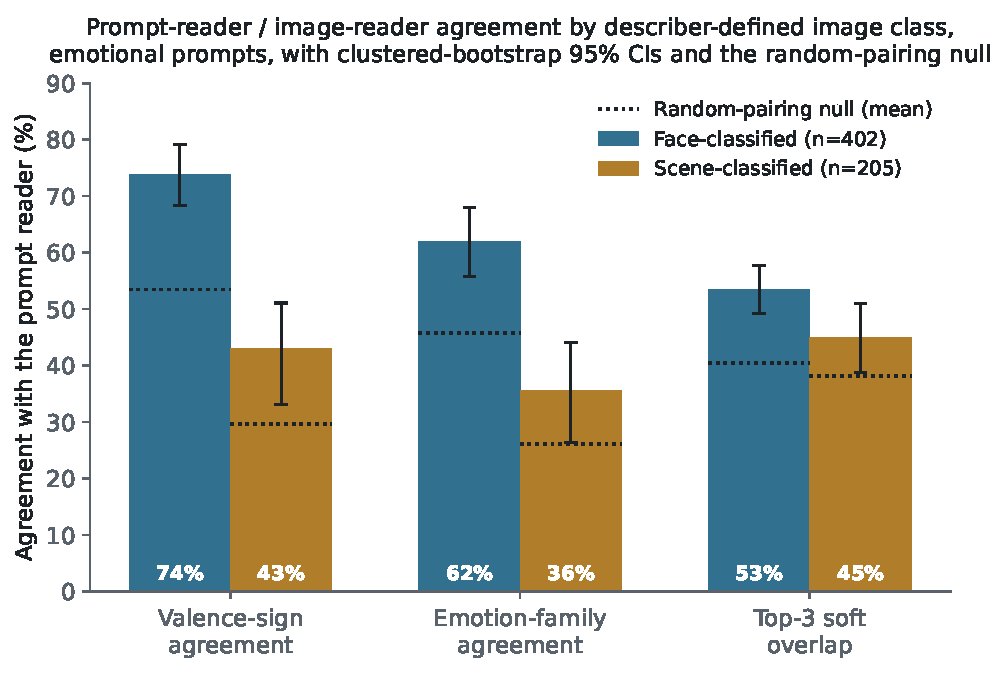
\includegraphics[width=\textwidth]{fig1_face_vs_scene}
\caption{Agreement of the image reader with the prompt reader on the emotional prompts, split by the describer-defined class of the drawing. Error bars are clustered-bootstrap 95\% intervals. The dotted line in each cell is that cell's random-pairing null.}
\label{fig:facescene}
\end{figure}

% GENERATED by emoviz/export_tex.py — do not edit
\begin{table}[htbp]
\centering
\footnotesize
\caption{Face-classified versus scene-classified drawings on the emotional prompts: agreement with 95\% clustered-bootstrap CIs, the difference with its CI, and the clustered permutation p (10,000 draws; significance.py).}
\label{tab:difference}
\begin{tabular}{lllll}
\toprule
Measure & Face ($n$=402) & Scene ($n$=205) & Difference (pp) & Perm.\ $p$ \\
\midrule
Valence-sign agreement & 73.9\% [68.3, 79.2] & 42.9\% [33.1, 51.1] & +30.9~pp [+22.6, +40.6] & 0.0001 \\
Family agreement & 61.9\% [55.8, 68.0] & 35.6\% [26.4, 44.1] & +26.3~pp [+18.4, +35.3] & 0.0001 \\
\bottomrule
\end{tabular}
\end{table}


\section{Distinct prompts and the multiple-comparison correction}
\label{sec:results-robustness}

Because \nRepeats{} records repeat an earlier prompt, Table~\ref{tab:distinct} re-runs the main table with only each prompt's first occurrence kept. That leaves \nDistinct{} records, \nDistinctEmo{} of them emotional. The overall and the face results hold: the \DistFaceN{} face-classified records among the distinct prompts give \DistFaceSignObs{} on valence sign ($z$ = \DistFaceSignZ{}) and \DistFaceFamObs{} on family ($z$ = \DistFaceFamZ{}). The scene row loses a good part of its margin. For the \DistSceneN{} scene-classified records among them, valence sign drops to \DistSceneSignObs{} ($z$ = \DistSceneSignZ{}) and family to \DistSceneFamObs{} ($z$ = \DistSceneFamZ{}).

Table~\ref{tab:holm} runs Holm--Bonferroni over all \HolmM{} of the $z$-scores that are not degenerate. \HolmSurvive{} pass at the family-wise 0.05 level and \HolmFail{} fail. The survivors include the full-sample cells of the emotional subset and of both image classes, and the distinct-prompt cells of the emotional subset and of the face class, so every cell reported so far survives except one. Most of the failures were expected to sit at chance anyway: the neutral-labelled control in both blocks, and the valence--arousal and overlap cells of the two single-valence subsets. The one failure among the reported cells is the scene family cell of the distinct-prompt block at $z$ = \DistSceneFamZ{}. It was expected to be informative, and is treated as suggestive only.

% GENERATED by emoviz/export_tex.py — do not edit
\begin{table}[htbp]
\centering
\small
\caption{The same analysis on the 763 distinct prompts only (first occurrence of each prompt text kept), a check against pseudo-replication from the 249 repeated prompts.}
\label{tab:distinct}
\begin{tabular}{lrrrl}
\toprule
Subset / measure & Observed & Null & $z$ & 95\% CI \\
\midrule
\textbf{Emotional prompts} ($n$=452; sign $n$=394) &  &  &  &  \\
Valence--arousal similarity & 83.0\% & 76.5\% & +10.6 & [81.5, 84.4] \\
Valence-sign agreement & 62.2\% & 44.4\% & +9.9 & [57.2, 67.0] \\
Family agreement & 51.3\% & 37.2\% & +9.3 & [46.7, 56.0] \\
Top-3 soft overlap & 48.9\% & 37.7\% & +10.8 & [45.9, 51.9] \\
\midrule
\textbf{\quad face-classified} ($n$=319; sign $n$=284) &  &  &  &  \\
Valence--arousal similarity & 83.5\% & 75.5\% & +9.7 & [81.7, 85.2] \\
Valence-sign agreement & 71.8\% & 51.0\% & +8.4 & [66.4, 77.0] \\
Family agreement & 59.9\% & 43.0\% & +8.1 & [54.2, 65.2] \\
Top-3 soft overlap & 51.8\% & 38.4\% & +9.7 & [48.1, 55.4] \\
\midrule
\textbf{\quad scene-classified} ($n$=133; sign $n$=110) &  &  &  &  \\
Valence--arousal similarity & 81.8\% & 78.9\% & +3.6 & [79.5, 83.8] \\
Valence-sign agreement & 37.3\% & 27.1\% & +3.5 & [28.1, 46.2] \\
Family agreement & 30.8\% & 24.1\% & +2.6 & [23.3, 38.4] \\
Top-3 soft overlap & 41.7\% & 36.7\% & +3.1 & [36.9, 46.5] \\
\midrule
\textbf{Neutral-labelled prompts} ($n$=311; sign $n$=0) &  &  &  &  \\
Valence--arousal similarity & 76.6\% & 76.4\% & +1.1 & -- \\
Valence-sign agreement & 0.0\% & 0.0\% & n/a & degenerate \\
Family agreement & 27.7\% & 27.7\% & n/a & degenerate \\
Top-3 soft overlap & 31.4\% & 31.1\% & +0.8 & -- \\
\bottomrule
\end{tabular}
\end{table}

% GENERATED by emoviz/export_tex.py — do not edit
\begin{table}[htbp]
\centering
\footnotesize
\caption{Multiple-comparison control over the 36 non-degenerate $z$-scores the analysis prints (12 degenerate ones excluded). Two-sided $p$ by the normal approximation; Holm--Bonferroni at family-wise 0.05: 26 survive, 10 do not.}
\label{tab:holm}
\begin{tabular}{lp{0.78\textwidth}}
\toprule
Outcome & Tests \\
\midrule
Do not survive & DISTINCT negative prompts overlap z+2.7; DISTINCT scene images family z+2.6; FULL positive prompts overlap z+2.3; FULL negative prompts va z+2.1; DISTINCT positive prompts overlap z+1.9; DISTINCT negative prompts va z+1.6; DISTINCT non-emotional va z+1.1; DISTINCT non-emotional overlap z+0.8; FULL non-emotional va z+0.3; FULL non-emotional overlap z+0.0 \\
Survive & the remaining 26, including every headline (emotional, face and scene on all four measures; distinct-prompt emotional and face) \\
\bottomrule
\end{tabular}
\end{table}


\section{Specificity check: prompts the prompt reader labels neutral}
\label{sec:results-control}

The specificity check uses the \CtrlN{} prompts that the prompt reader labelled neutral. Only one measure can move here. Valence sign has a numerator and a denominator of zero on this subset, and the family rate is exactly its null, \CtrlFamObs{}, because every prompt has the same label and re-pairing the drawings cannot change how often the two labels coincide. Valence--arousal similarity does have a live null, and the observed value sits on it: \CtrlVaObs{} against \CtrlVaNull{}, with $z$ = \CtrlVaZ{} at record level and \CtrlVaZClustered{} when the null is clustered on prompt groups.

Table~\ref{tab:control} reports the control audit. \CtrlFlagged{} of the \CtrlN{} (\CtrlFlaggedPct{}) contain at least one word from a fixed lexicon of \CtrlLexicon{} everyday affect words, the commonest being \CtrlTopWords{}, and a further \CtrlNameOnly{} consist of nothing but the redaction placeholder. Removing them leaves a cleaned control of \CtrlCleanN{} records. On those the value is \CtrlCleanVaObs{} against \CtrlCleanVaNull{} ($z$ = \CtrlCleanVaZ{}), the same as before. The null's standard deviation here is only \CtrlVaSd{}, because the prompt-side points hardly vary between neutral prompts, so observed and expected were always going to land close together. The check passes, and weakly, for that reason.

% GENERATED by emoviz/export_tex.py — do not edit
\begin{table}[htbp]
\centering
\small
\caption{The specificity check on the prompts the text reader labels neutral. Only valence--arousal similarity is informative there (sign and family are degenerate: every prompt shares the neutral label). Cleaned control = minus the 2 records reduced to `[name]' and the 68 containing one of 66 plain affect words.}
\label{tab:control}
\begin{tabular}{lrrrrr}
\toprule
Control set & $n$ & VA observed & VA null & $z$ (record null) & $z$ (clustered null) \\
\midrule
All neutral-labelled prompts & 405 & 76.6\% & 76.5\% & +0.5 & -0.1 \\
Cleaned control & 335 & 76.6\% & 76.6\% & +0.0 & -0.6 \\
\bottomrule
\end{tabular}
\end{table}


\section{Two image readers, like for like}
\label{sec:results-method}

Figure~\ref{fig:method} and Table~\ref{tab:method} score the two image readers under identical conditions: one prompt reader, the same \McN{} emotional records, the four measures and one set of random re-pairings. On family agreement describe-then-extract reaches \McDeFam{} and direct CLIP \McClipFam{}. The difference of \McDiffFamPp{} has a clustered interval of \McDiffFamCi{}, the cluster sign-flip test puts $p$ at \McClusterFamP{}, and the exact McNemar test, which takes every record as independent and so errs on the optimistic side, gives $p$ = \McMcNemarFamP{}. Valence sign goes the same way, \McDeSign{} against \McClipSign{} (\McDiffSignPp{}, CI \McDiffSignCi{}), as do overlap (\McDeOvlp{} against \McClipOvlp{}) and valence--arousal similarity (\McDeVa{} against \McClipVa{}). Counting records, \McFamB{} of the \McN{} are agreed on by describe-then-extract alone, \McFamC{} by direct CLIP alone, \McFamBoth{} by both readers and \McFamNeither{} by neither.

Two numbers in the table need a note. Direct CLIP's family $z$ is \McClipFamZ{}, above the \McDeFamZ{} of describe-then-extract, even though its rate is far lower. The reason is that its null sits lower and varies less. Direct CLIP returns neutral for \McClipNeutral{} of the \McN{} images, and an image read as neutral cannot agree by family with any emotional prompt the re-pairing hands it, so chance agreement is rare for it too. A $z$ measures a reader's distance from its own chance level, so the comparison between the readers rests on the paired tests on the rates above. The second number is the two image readers' own agreement, only \McReaderAgree{} on top-1 family. Table~\ref{tab:methodvone} is the first build's version of this comparison, run on \McVOneN{} records with the entailment model on the prompt side too and an earlier overlap formula, so its figures are not comparable with those of the main analysis. It is kept as history only and none of its figures is quoted.

\begin{figure}[htbp]
\centering
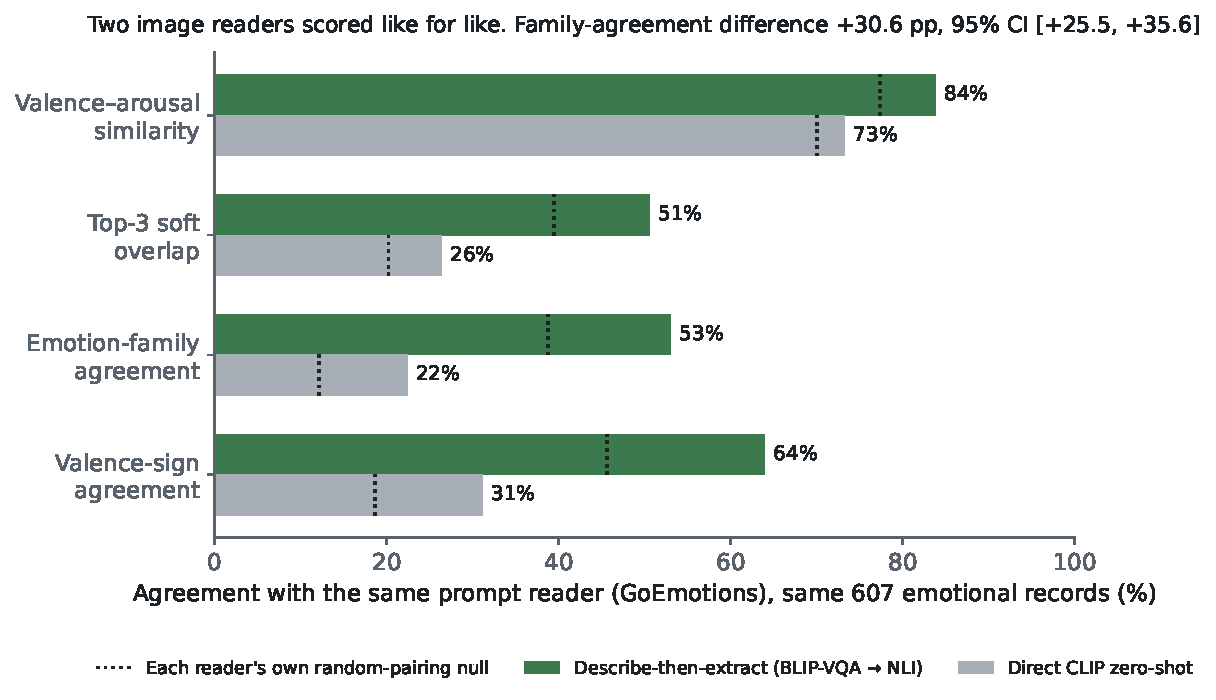
\includegraphics[width=\textwidth]{fig2_method_comparison}
\caption{The two image readers scored against one prompt reader on the same \McN{} emotional records. The dotted mark in each cell is that reader's own random-pairing null.}
\label{fig:method}
\end{figure}

{\setlength{\tabcolsep}{2.5pt}% GENERATED by emoviz/export_tex.py — do not edit
\begin{table}[htbp]
\centering
\scriptsize
\caption{Two image readers scored like for like against the same prompt reader (GoEmotions) on the same 607 emotional records with the same measures and the same 300 re-pairings. $b$ = records only describe-then-extract agrees on; $c$ = records only direct CLIP agrees on. The exact McNemar $p$ treats records as independent and is optimistic ($3.4\times10^{-35}$ for family); the cluster sign-flip randomisation (20,000 draws) respects prompt groups.}
\label{tab:method}
\begin{tabular}{lrrrrrr}
\toprule
Measure & Describe→extract & null & $z$ & Direct CLIP & null & $z$ \\
\midrule
Valence--arousal similarity & 83.8\% & 77.3\% & +12.2 & 73.3\% & 70.1\% & +10.2 \\
Valence-sign agreement & 64.0\% & 45.6\% & +11.1 & 31.1\% & 18.6\% & +9.9 \\
Family agreement & 53.0\% & 38.8\% & +10.3 & 22.4\% & 12.2\% & +11.1 \\
Top-3 soft overlap & 50.6\% & 39.4\% & +11.6 & 26.4\% & 20.2\% & +11.2 \\
\midrule
Paired family test & $b$=218, $c$=32 &  &  & diff +30.6~pp & CI [+25.5, +35.6] & cluster $p<0.001$ \\
Paired valence-sign test & $b$=204, $c$=30 &  &  & diff +32.8~pp & CI [+27.4, +38.2] & cluster $p<0.001$ \\
\bottomrule
\end{tabular}
\end{table}
}
% GENERATED by emoviz/export_tex.py — do not edit
\begin{table}[htbp]
\centering
\small
\caption{The earlier (v1) comparison as published in the build log: prompt side read by BART-MNLI, the 608 records of the v1 lexicon rule, and a different overlap formula. Kept as a record; not comparable with Table~\ref{tab:headline}.}
\label{tab:methodvone}
\begin{tabular}{lrr}
\toprule
Measure & Describe→extract & Direct CLIP \\
\midrule
Family agreement & 49.3\% & 25.3\% \\
Top-3 soft overlap & 48.6\% & 22.8\% \\
Valence--arousal similarity & 83.7\% & 74.2\% \\
\bottomrule
\end{tabular}
\end{table}


\section{Consistency across repeated prompts}
\label{sec:results-consistency}

Repeated prompts form \nGroups{} groups, which cover \nGroupRecords{} records. \nPairGroups{} of them are pairs. Figure~\ref{fig:consistency} and Table~\ref{tab:consistency} report how often the drawings in a group get the same reading. Averaged over groups, the share of a group's drawings given its modal family is \ConsFam{}, with a bootstrap interval over groups of \ConsFamCi{}. The permutation null shuffles image families over every analysed record and re-cuts the same groups, and it gives \ConsFamNull{} with a standard deviation of \ConsFamNullSd{}, so $z$ = \ConsFamZ{} and the permutation $p$ is \ConsFamP{}. On valence sign the within-group share is \ConsVal{} against \ConsValNull{} ($z$ = \ConsValZ{}). Groups in which every drawing received one family, the fully consistent ones, number \ConsFull{} of \nGroups{} (\ConsFullPct{}), where \ConsFullNull{} would be expected by chance ($z$ = \ConsFullZ{}). For the \nPairGroups{} pairs the share can only be one half or one, which puts a floor under the mean.

The largest group is the single word ``happy'', drawn \ConsHappyN{} times. Of those drawings the image reader returned joy for \ConsHappyJoy{}, neutral for \ConsHappyNeutral{} and surprise for \ConsHappySurprise{}, and Figure~\ref{fig:happygrid} lays out a selection of them with the reader's family printed under each.

\begin{figure}[htbp]
\centering
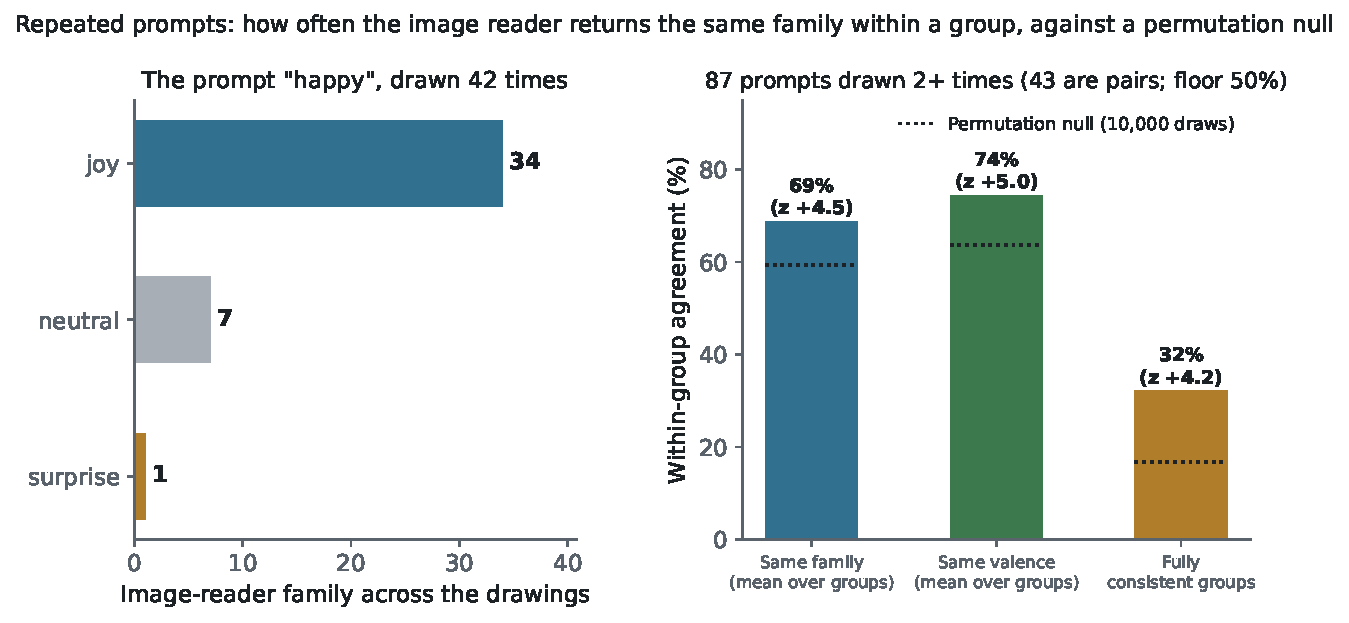
\includegraphics[width=\textwidth]{fig4_consistency}
\caption{Repeated prompts. Left: the image reader's top-1 family over the \ConsHappyN{} drawings of ``happy''. Right: for all \nGroups{} repeated prompts, the share of a group's drawings given its modal family, with the permutation null.}
\label{fig:consistency}
\end{figure}

\begin{figure}[htbp]
\centering
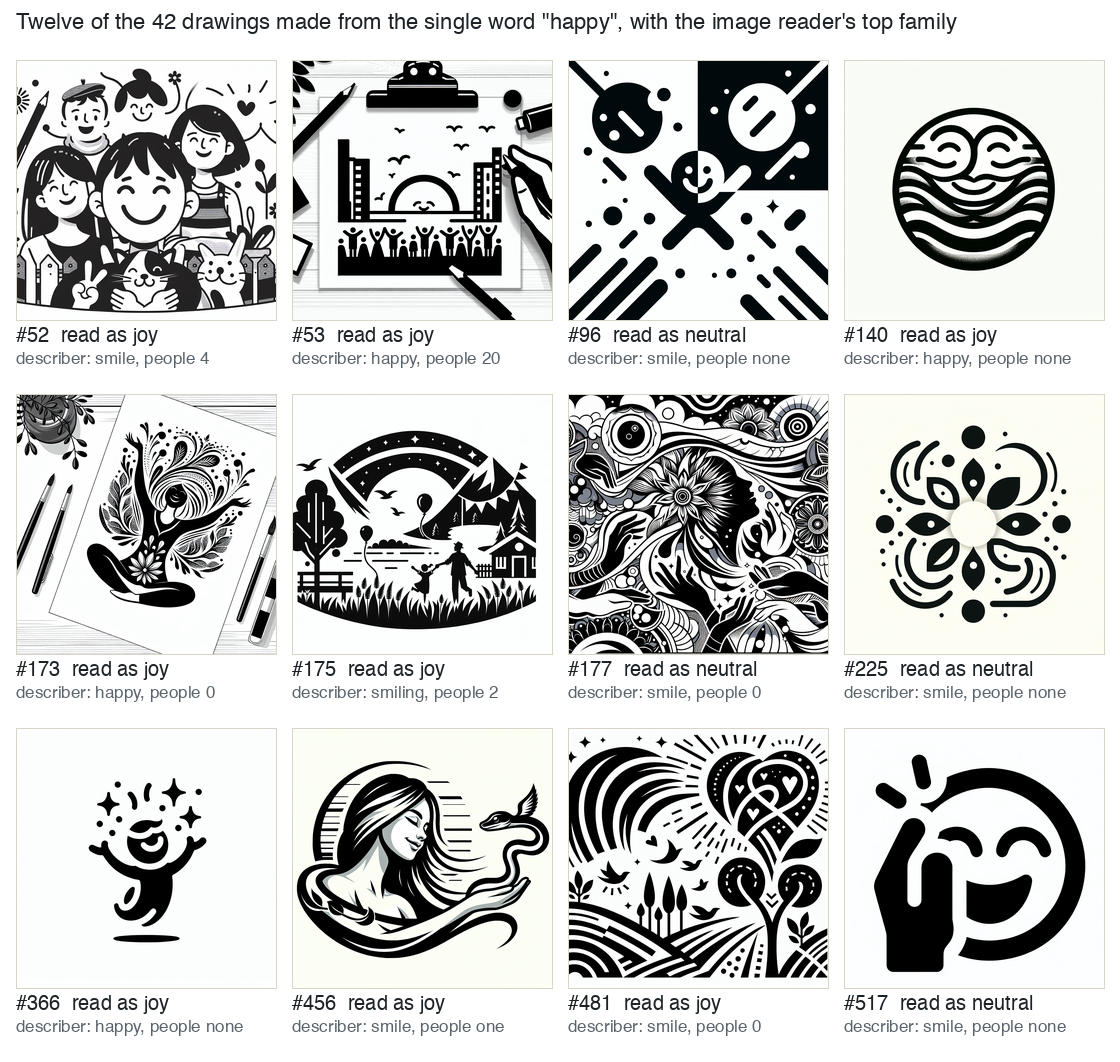
\includegraphics[width=\textwidth]{fig_happy_grid}
\caption{Twelve of the \ConsHappyN{} drawings made from the prompt ``happy'', each with the family the image reader returned for it.}
\label{fig:happygrid}
\end{figure}

% GENERATED by emoviz/export_tex.py — do not edit
\begin{table}[htbp]
\centering
\small
\caption{Within-group agreement of the image reader across the 87 prompts drawn two or more times (336 records; 43 groups are pairs, whose modal agreement cannot fall below 50\%), against a permutation null that shuffles the image readings over all 1,012 analysed records and re-cuts them into the same groups (10,000 draws, seed 7).}
\label{tab:consistency}
\begin{tabular}{lrrrr}
\toprule
Quantity & Observed & Null mean (sd) & $z$ & $p$ \\
\midrule
Same family, mean over groups & 68.8\% & 59.4\% (2.1\%) & +4.5 & $1.0\times10^{-4}$ \\
Same valence, mean over groups & 74.5\% & 63.7\% (2.1\%) & +5.0 & $1.0\times10^{-4}$ \\
Fully consistent groups (of 87) & 28 & 14.5 (3.2) & +4.2 & $2.0\times10^{-4}$ \\
\bottomrule
\end{tabular}
\end{table}


\section{Per-family agreement}
\label{sec:results-families}

Figure~\ref{fig:confusion} and Table~\ref{tab:confusion} tabulate the image reader's family against the prompt reader's for the \nEmotional{} emotional records, and Table~\ref{tab:families} gives the marginals of both readers over all \nAnalysed{} analysed records. Joy dominates the prompt side. It accounts for \RecJoyN{} of the emotional prompts, sadness for \RecSadnessN{} and surprise for \RecSurpriseN{}, while fear (\RecFearN{}), anger (\RecAngerN{}) and disgust (\RecDisgustN{}) are rare. Recall by prompt family is defined per row: of the prompts the prompt reader assigns to a family, the share whose drawing the image reader also assigns to it. Joy has recall \RecJoy{} (CI \RecJoyCi{}) and sadness \RecSadness{} (CI \RecSadnessCi{}); surprise is at \RecSurprise{} (CI \RecSurpriseCi{}), anger at \RecAnger{} on only \RecAngerN{} prompts and fear at \RecFear{} on \RecFearN{}. Disgust never comes back from the image reader. Fear comes back \famImageFear{} times in \nAnalysed{} records.

Table~\ref{tab:kappa} gives Cohen's kappa for family agreement. For the emotional prompts it is \KappaEmo{} (CI \KappaEmoCi{}), the face-classified records give \KappaFace{} and the scene-classified \KappaScene{}, which the Landis--Koch bands call \KappaEmoBand{}, \KappaFaceBand{} and \KappaSceneBand{} in that order. In practice family agreement can be read on three families, joy, sadness and neutral. Anger comes fourth, and it is too rare on the prompt side, as are fear and disgust, for a claim about any one of the three.

\begin{figure}[htbp]
\centering
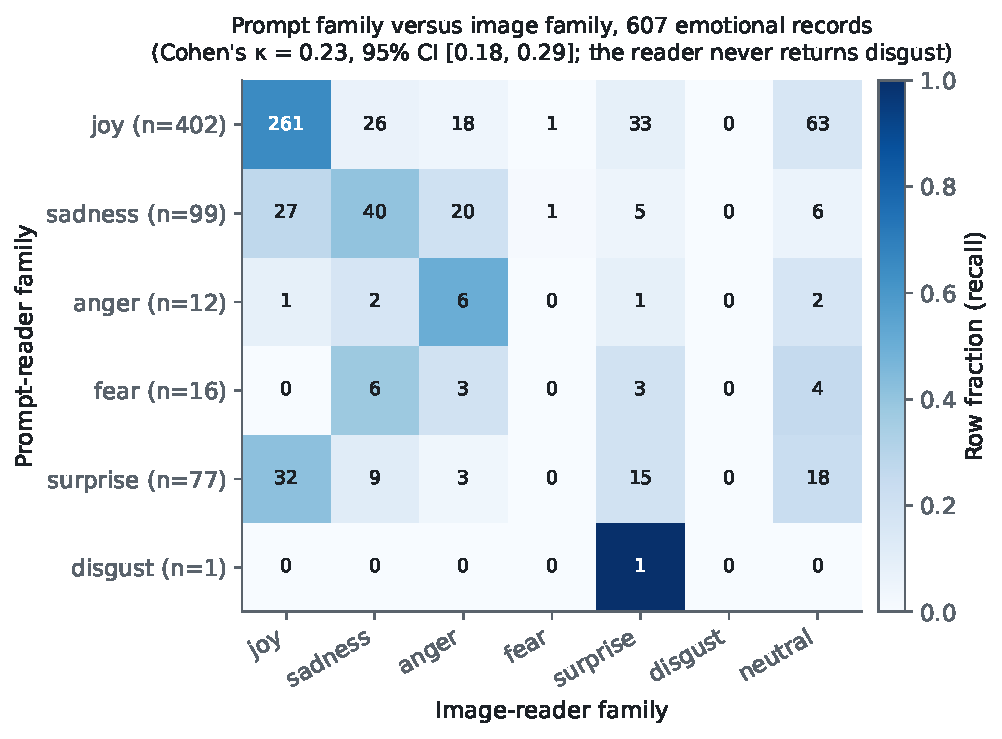
\includegraphics[width=0.85\textwidth]{fig6_confusion}
\caption{Prompt-reader family (rows) crossed with image-reader family (columns) on the \nEmotional{} emotional records. Each cell holds a count, and the shading is the share of the row.}
\label{fig:confusion}
\end{figure}

% GENERATED by emoviz/export_tex.py — do not edit
\begin{table}[htbp]
\centering
\scriptsize
\caption{Prompt-reader family (rows) against image-reader family (columns) on the 607 emotional records. Recall = row diagonal share, with a clustered-bootstrap 95\% CI. Cohen's $\kappa$ = 0.23 [0.18, 0.29]. The image reader never returns disgust and returns fear 4 times in 1,012 records.}
\label{tab:confusion}
\begin{tabular}{lrrrrrrrrl}
\toprule
Prompt \textbackslash{} image & joy & sadness & anger & fear & surprise & disgust & neutral & $n$ & Recall [CI] \\
\midrule
joy & 261 & 26 & 18 & 1 & 33 & 0 & 63 & 402 & 64.9\% [59, 70] \\
sadness & 27 & 40 & 20 & 1 & 5 & 0 & 6 & 99 & 40.4\% [31, 51] \\
anger & 1 & 2 & 6 & 0 & 1 & 0 & 2 & 12 & 50.0\% [22, 78] \\
fear & 0 & 6 & 3 & 0 & 3 & 0 & 4 & 16 & 0.0\% [0, 0] \\
surprise & 32 & 9 & 3 & 0 & 15 & 0 & 18 & 77 & 19.5\% [11, 28] \\
disgust & 0 & 0 & 0 & 0 & 1 & 0 & 0 & 1 & 0.0\% [0, 0] \\
\midrule
\textit{image total} & 321 & 83 & 50 & 2 & 58 & 0 & 93 & 607 &  \\
\bottomrule
\end{tabular}
\end{table}

% GENERATED by emoviz/export_tex.py — do not edit
\begin{table}[htbp]
\centering
\small
\caption{Cohen's $\kappa$ for family agreement (7 families), with clustered-bootstrap 95\% CIs and the Landis \& Koch (1977) band. The neutral-labelled subset is degenerate ($\kappa$ = 0 by construction) and is omitted.}
\label{tab:kappa}
\begin{tabular}{lrrll}
\toprule
Subset & $n$ & $\kappa$ & 95\% CI & Band \\
\midrule
emotional & 607 & 0.23 & [0.18, 0.29] & fair \\
face & 402 & 0.30 & [0.23, 0.37] & fair \\
scene & 205 & 0.13 & [0.06, 0.19] & slight \\
all analysed & 1012 & 0.21 & [0.16, 0.25] & fair \\
distinct emotional & 452 & 0.23 & [0.17, 0.29] & fair \\
distinct face & 319 & 0.29 & [0.21, 0.37] & fair \\
distinct scene & 133 & 0.09 & [0.01, 0.17] & slight \\
\bottomrule
\end{tabular}
\end{table}

% GENERATED by emoviz/export_tex.py — do not edit
\begin{table}[htbp]
\centering
\small
\caption{Top-1 family marginals of the two readers over all 1,012 analysed records.}
\label{tab:families}
\begin{tabular}{lrr}
\toprule
Family & Prompt reader & Image reader \\
\midrule
joy & 402 & 461 \\
sadness & 99 & 141 \\
anger & 12 & 89 \\
fear & 16 & 4 \\
surprise & 77 & 108 \\
disgust & 1 & 0 \\
neutral & 405 & 209 \\
\bottomrule
\end{tabular}
\end{table}


\section{The describer}
\label{sec:results-describer}

Table~\ref{tab:describer} tabulates, for all \nAnalysed{} records, the people count the describer gives against whether its expression answer contains an expression word, so the cells separate the records with a person and an expression word from those with only one of the two and those with neither. The expression question never gets a blank. For \DescNoPeopleExpr{} records it names an expression while its own people count says nobody is there. The scene-classified records number \DescSceneN{}, and for \DescScenePeopleZero{} of them the people count is zero, yet an expression word is present in \DescScenePeopleZeroExpr{} of those. Of the \DescScenePeopleZero{} records with no reported person, \DescSceneSmile{} (\DescSceneSmilePct{}) give ``smile'', ``smiling'' or ``happy'' as the expression. Figure~\ref{fig:noperson} shows four such drawings with all five answers. The smile rate is given with both denominators: \DescSmileAll{} over all \nAnalysed{} analysed records, \DescSmileFace{} over the \nFaceAll{} face-classified ones.

Copy rate means the share of records on which the image reader returns the family of the describer's own expression answer. On the strict definition the answer must be an emotion word. That is so for \DescBareStrictN{} records, \DescBareStrictPct{} of the corpus, and for those records the family the image reader returns is the family of the describer's own word \DescCopyStrict{} of the time. The broad definition also counts a facial action, ``smile'' or ``crying'' for instance, and covers \DescBareBroadN{} records. On it the copy rate is \DescCopyBroad{} overall, \DescCopyBroadPeople{} when the describer reports a person and \DescCopyBroadPeopleZero{} when it reports none. With the ``0 people'' token in the description, the reading is pulled towards neutral.

% GENERATED by emoviz/export_tex.py — do not edit
\begin{table}[htbp]
\centering
\small
\caption{The describer's answers on all 1,012 analysed records: people count crossed with whether the facial-expression answer contains an expression word. The face rule is the top-left cell. Of the 421 scene-classified records, 414 report no people and 406 of those still contain an expression word (332 answer smile, smiling or happy).}
\label{tab:describer}
\begin{tabular}{lrr}
\toprule
 & Expression word present & Expression word absent \\
\midrule
People $\geq 1$ & 591 & 7 \\
People $= 0$ & 406 & 8 \\
\bottomrule
\end{tabular}
\end{table}


\begin{figure}[htbp]
\centering
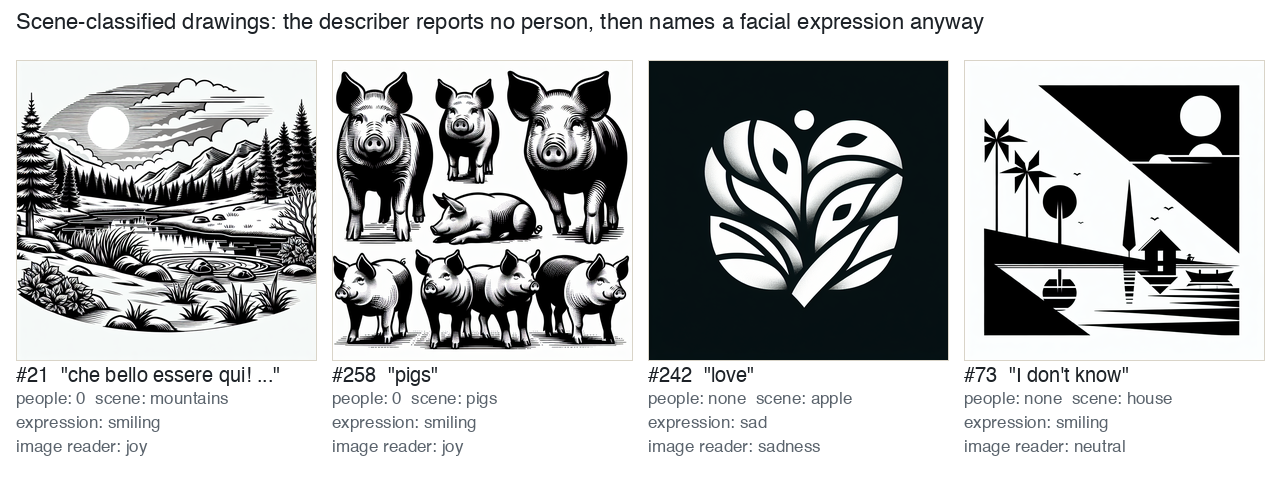
\includegraphics[width=\textwidth]{fig_no_person_expression}
\caption{Four scene-classified drawings for which the describer reported no person and still named a facial expression, each with its five answers as given.}
\label{fig:noperson}
\end{figure}

\section{Error taxonomy}
\label{sec:results-taxonomy}

The taxonomy covers the emotional records where each reader gives its top family a score of at least 0.8 and the two families differ. There are \TaxN{} of them, covering \TaxDistinct{} distinct prompts. The intention was to sample 40, but fewer than that qualified, so every one was examined. Figure~\ref{fig:taxonomy} and Table~\ref{tab:taxonomy} count the primary failure mode, which was assigned by looking at the drawing. The describer is behind \TaxDescriber{} of the \TaxN{}, \TaxA{} of those because a face or an expression it reported is not in the drawing and \TaxB{} because it misread one that is. The image reader accounts for \TaxReader{}, where the description was fair to the drawing and the entailment step still returned another family. \TaxPrompt{} trace to the prompt side, \TaxD{} of them mixed or ambiguous prompts and \TaxF{} a prompt the prompt reader mislabelled, and \TaxGenerator{} to the generator, where the drawing does not depict what the prompt says. Record 137, ``i am excited'', drawn as a screaming face, is one of the \TaxGenerator{} generator cases.

The table shows two patterns. A people count of zero goes with the invented-expression mode, since \TaxPeopleZero{} of the \TaxN{} records have the ``0 people'' tag and most of the \TaxA{} invented-expression records are among them. One mechanism accounts for the joy-to-neutral cell. ``grateful'' and ``calm but tired'' are two of the prompts in it, and both name a low-arousal positive state that none of the seven families has room for, so the describer's answer is ``calm'' or ``smile'' and the image reader returns neutral. The automatic detector for mixed prompts looked for connectives such as ``but'' and ``although''. It caught none of the \TaxD{} mixed prompts, because visitors tend to list feelings with no connective at all, as in ``tired proud happy'', and a detector that looks for a list would do better.

\begin{figure}[htbp]
\centering
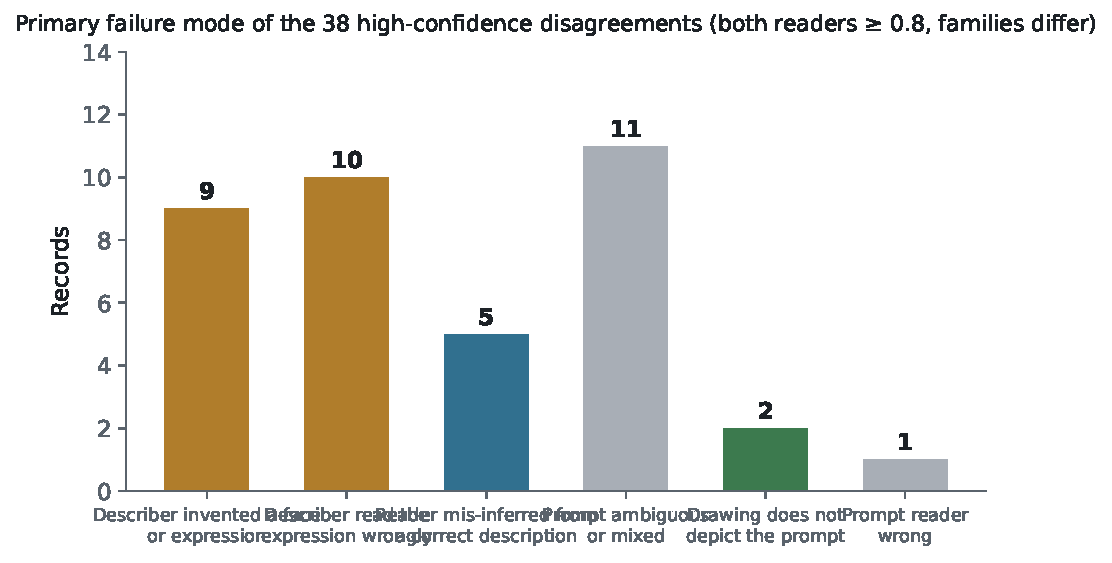
\includegraphics[width=0.95\textwidth]{fig7_error_taxonomy}
\caption{Primary failure mode of the \TaxN{} high-confidence disagreements. Each was assigned by looking at the drawing.}
\label{fig:taxonomy}
\end{figure}

% GENERATED by emoviz/export_tex.py — do not edit
\begin{table}[htbp]
\centering
\small
\caption{Primary failure mode of the 38 high-confidence disagreements (both readers' top-1 score $\geq 0.8$, families differ), assigned from the drawing. Describer faults (a+b) = 19; image reader (c) = 5; prompt side (d+f) = 12; generator (e) = 2.}
\label{tab:taxonomy}
\begin{tabular}{lp{0.55\textwidth}rl}
\toprule
Mode & Description & $n$ & Exemplar ids \\
\midrule
(a) & describer invented a face or expression where none is drawn & 9 & 18, 19, 242 \\
(b) & describer read the expression wrongly & 10 & 39, 192, 202 \\
(c) & reader mis-inferred from a correct description & 5 & 89, 107, 231 \\
(d) & prompt ambiguous or mixed & 11 & 65, 66, 93 \\
(e) & drawing does not depict the prompt & 2 & 137, 771 \\
(f) & prompt reader wrong & 1 & 436 \\
\bottomrule
\end{tabular}
\end{table}


\section{Description-template ablation}
\label{sec:results-ablation}

The template ablation is in Table~\ref{tab:ablation} and Figure~\ref{fig:ablation}, one row per altered description template. Only the entailment stage was re-run. As a control the unmodified template was re-run through the same code path, and the number of records whose top-1 reading changed was \AblControlChanged{}, so the re-run is exact and every difference in the table comes from the template change. The unmodified row reproduces Section~\ref{sec:results-overall}.

Dropping the expression sentence removes most of the agreement. For the emotional prompts, family agreement goes from \FullEmoFamObs{} down to \AblDropExpressionEmoFamObs{}, where the null is \AblDropExpressionEmoFamNull{} ($z$ = \AblDropExpressionEmoFamZ{}), and valence sign from \FullEmoSignObs{} down to \AblDropExpressionEmoSignObs{}, null \AblDropExpressionEmoSignNull{} ($z$ = \AblDropExpressionEmoSignZ{}). The face-classified records alone end at \AblDropExpressionFaceSignObs{} on valence sign. With the expression sentence gone, the image reader's output piles up on two families, surprise on \AblDropExpressionSurprise{} of the \nAnalysed{} records and neutral on \AblDropExpressionNeutral{}. Holding the expression word at ``unclear'' for every record collapses the ladder in the same way, with family agreement at \AblFixedExpressionEmoFamObs{} ($z$ = \AblFixedExpressionEmoFamZ{}). The other clauses matter less. Taking out the action clause, or the posture or scene clause, instead shifts family agreement by between one and three points, to \AblDropActionEmoFamObs{}, \AblDropPostureEmoFamObs{} and \AblDropSceneEmoFamObs{}. Dropping the people count raises the rates and the nulls together, the scene valence-sign cell going to \AblDropPeopleSceneSignObs{} against \AblDropPeopleSceneSignNull{} ($z$ = \AblDropPeopleSceneSignZ{}). Without the ``0 people'' token holding scene readings near neutral, the invented smile reads as joy, and joy is the top family of most emotional prompts.

Under the people-aware template the whole description becomes ``A drawing showing \{scene\}.'' for any record whose people count is zero, and nothing else changes. The face rows cannot change under it. They stay at \AblPeopleAwareFaceSignObs{} and \AblPeopleAwareFaceFamObs{}, identical to the unmodified template by construction, because a face-classified record always has a person reported and so keeps its full description. The scene rows both fall to their nulls, on valence sign \AblPeopleAwareSceneSignObs{} where the null is \AblPeopleAwareSceneSignNull{} ($z$ = \AblPeopleAwareSceneSignZ{}), and on family \AblPeopleAwareSceneFamObs{} where the null is \AblPeopleAwareSceneFamNull{} ($z$ = \AblPeopleAwareSceneFamZ{}). Putting the action and posture clauses back for those records gives the scene cells \AblPeopleAwareNoExpressionSceneSignObs{} on valence sign, null \AblPeopleAwareNoExpressionSceneSignNull{} ($z$ = \AblPeopleAwareNoExpressionSceneSignZ{}), and \AblPeopleAwareNoExpressionSceneFamObs{} on family, null \AblPeopleAwareNoExpressionSceneFamNull{} ($z$ = \AblPeopleAwareNoExpressionSceneFamZ{}). Taken over every emotional prompt, the people-aware template gives \AblPeopleAwareEmoSignObs{} on valence sign ($z$ = \AblPeopleAwareEmoSignZ{}) and \AblPeopleAwareEmoFamObs{} on family ($z$ = \AblPeopleAwareEmoFamZ{}).

\begin{figure}[htbp]
\centering
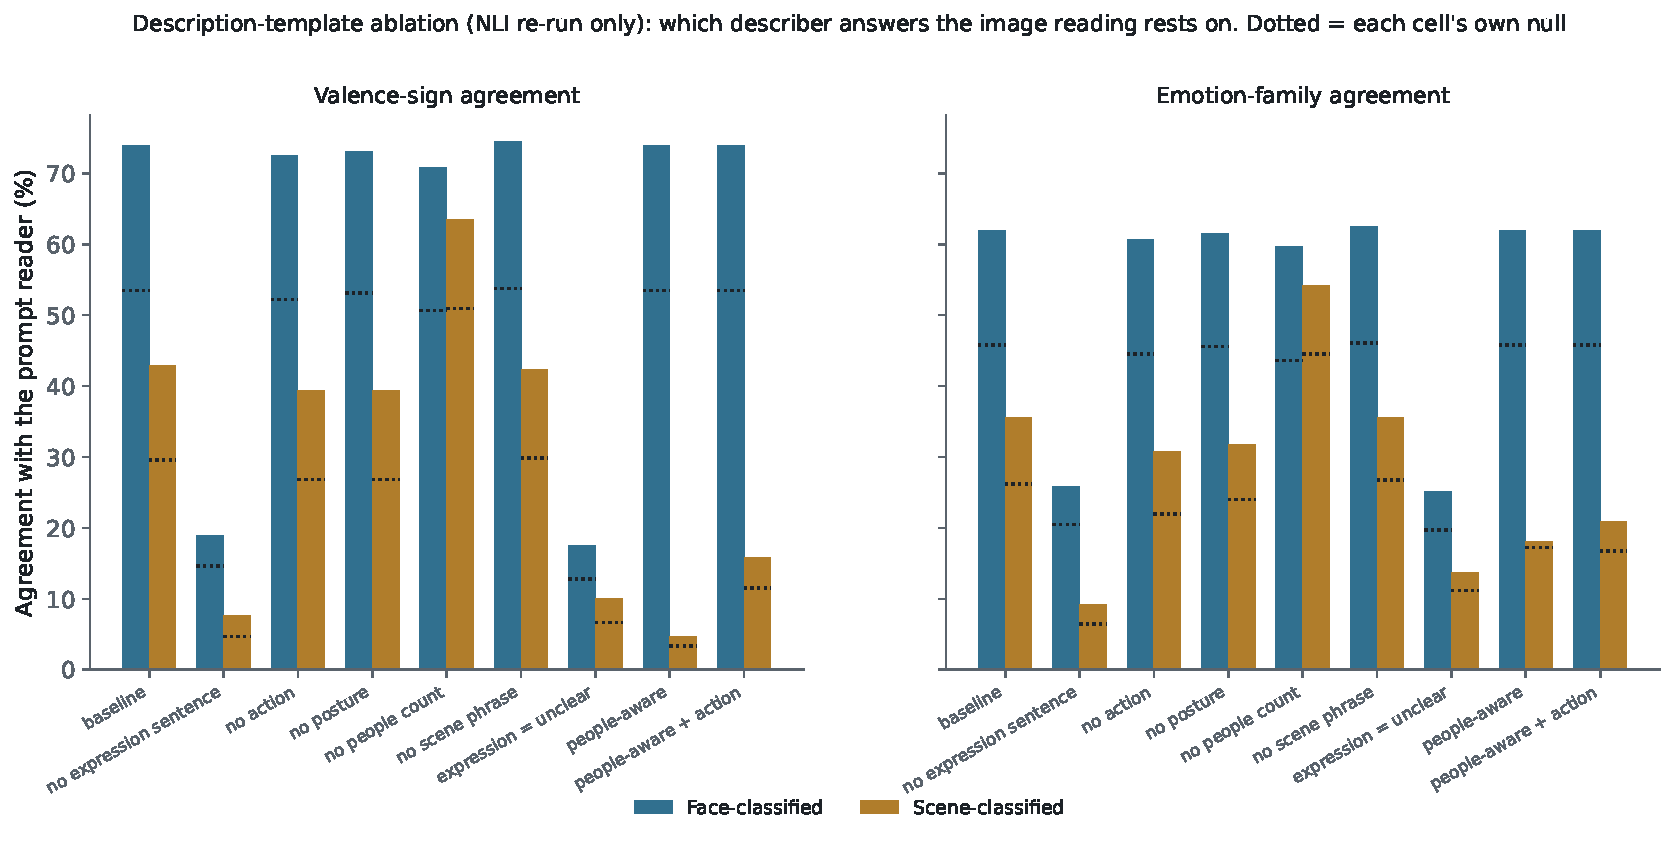
\includegraphics[width=\textwidth]{fig8_ablation}
\caption{Description-template ablation with only the entailment stage re-run. Valence-sign and family agreement by image class under each template. The dotted line in each cell is that cell's random-pairing null.}
\label{fig:ablation}
\end{figure}

% GENERATED by emoviz/export_tex.py — do not edit
\begin{table}[htbp]
\centering
\footnotesize
\caption{Description-template ablation: the NLI stage re-run on descriptions rebuilt from the cached describer answers with one clause removed or fixed; the prompt side and the null procedure unchanged. Valence-sign and family agreement per variant on the emotional prompts and their face/scene halves.}
\label{tab:ablation}
\begin{tabular}{llrrrrrrr}
\toprule
Variant & Subset & $n$ & Sign obs & null & $z$ & Family obs & null & $z$ \\
\midrule
baseline & emotional & 607 & 64.0\% & 45.6\% & +11.1 & 53.0\% & 38.8\% & +10.3 \\
 & face & 402 & 73.9\% & 53.5\% & +10.4 & 61.9\% & 45.8\% & +10.3 \\
 & scene & 205 & 42.9\% & 29.6\% & +5.8 & 35.6\% & 26.2\% & +4.4 \\
\midrule
drop\_expression & emotional & 607 & 15.3\% & 11.4\% & +5.1 & 20.3\% & 16.6\% & +3.8 \\
 & face & 402 & 18.9\% & 14.7\% & +3.8 & 25.9\% & 20.5\% & +3.8 \\
 & scene & 205 & 7.6\% & 4.7\% & +2.7 & 9.3\% & 6.4\% & +2.2 \\
\midrule
drop\_action & emotional & 607 & 61.9\% & 43.9\% & +11.0 & 50.6\% & 36.7\% & +10.3 \\
 & face & 402 & 72.5\% & 52.2\% & +10.4 & 60.7\% & 44.5\% & +10.4 \\
 & scene & 205 & 39.4\% & 26.8\% & +5.6 & 30.7\% & 21.9\% & +4.6 \\
\midrule
drop\_posture & emotional & 607 & 62.3\% & 44.5\% & +10.7 & 51.4\% & 37.9\% & +9.7 \\
 & face & 402 & 73.1\% & 53.1\% & +10.0 & 61.4\% & 45.6\% & +10.1 \\
 & scene & 205 & 39.4\% & 26.8\% & +5.6 & 31.7\% & 24.0\% & +3.6 \\
\midrule
drop\_people & emotional & 607 & 68.5\% & 50.7\% & +10.8 & 57.8\% & 43.7\% & +9.9 \\
 & face & 402 & 70.8\% & 50.7\% & +10.4 & 59.7\% & 43.6\% & +10.3 \\
 & scene & 205 & 63.5\% & 50.9\% & +5.0 & 54.1\% & 44.5\% & +3.8 \\
\midrule
drop\_scene & emotional & 607 & 64.2\% & 46.0\% & +10.7 & 53.4\% & 39.2\% & +9.8 \\
 & face & 402 & 74.4\% & 53.8\% & +10.4 & 62.4\% & 46.1\% & +10.1 \\
 & scene & 205 & 42.4\% & 29.9\% & +5.6 & 35.6\% & 26.8\% & +3.9 \\
\midrule
fixed\_expression & emotional & 607 & 15.1\% & 10.8\% & +5.9 & 21.3\% & 17.5\% & +3.9 \\
 & face & 402 & 17.5\% & 12.8\% & +4.4 & 25.1\% & 19.7\% & +4.0 \\
 & scene & 205 & 10.0\% & 6.6\% & +2.8 & 13.7\% & 11.2\% & +1.5 \\
\midrule
people\_aware & emotional & 607 & 51.7\% & 36.9\% & +10.1 & 47.1\% & 34.5\% & +8.8 \\
 & face & 402 & 73.9\% & 53.5\% & +10.4 & 61.9\% & 45.8\% & +10.3 \\
 & scene & 205 & 4.7\% & 3.4\% & +1.6 & 18.0\% & 17.3\% & +0.6 \\
\midrule
people\_aware\_no\_expression & emotional & 607 & 55.3\% & 39.5\% & +10.5 & 48.1\% & 35.0\% & +9.6 \\
 & face & 402 & 73.9\% & 53.5\% & +10.4 & 61.9\% & 45.8\% & +10.3 \\
 & scene & 205 & 15.9\% & 11.6\% & +2.7 & 21.0\% & 16.8\% & +2.2 \\
\midrule
control\_full\_template & emotional & 607 & 64.0\% & 45.6\% & +11.1 & 53.0\% & 38.8\% & +10.3 \\
 & face & 402 & 73.9\% & 53.5\% & +10.4 & 61.9\% & 45.8\% & +10.3 \\
 & scene & 205 & 42.9\% & 29.6\% & +5.8 & 35.6\% & 26.2\% & +4.4 \\
\bottomrule
\end{tabular}
\end{table}


\section{Single-coder reliability check}
\label{sec:results-human}

The \HcN{} sampled drawings were coded from the contact sheets (the first is Figure~\ref{fig:codingsheet}), blind to the prompt, the description and both readings, marking for each one whether a person is drawn, whether a face can be read, the valence it gives and the family. Table~\ref{tab:humancheck} scores the pipeline against that coding with Wilson intervals. One person coded it once, so it is a judgement, not a reliability estimate.

The describer's people count agrees with the coder on \HcPeopleAcc{} of the sample, so it can tell whether anybody is drawn. The face rule cannot. Its accuracy against the coder's judgement of whether a face is readable is \HcFaceAcc{}, and it holds a recall of \HcFaceRec{} against a precision of \HcFacePrec{}: of the drawings it puts in the face class, fewer than half carry a face the coder could read. The ``smiling'' answers go the same way. Of the \HcSmileN{} in the sample, \HcSmileTrue{} have a readable positive face behind them and \HcSmileNoPerson{} have nobody drawn at all, which is the count of Section~\ref{sec:results-describer} met from the other side, by a person.

Against the coder's own reading of the drawings the image reader agrees on valence sign for \HcReaderSign{} of the records that have a sign, and on family for \HcReaderFam{} ($\kappa$ = \HcReaderKappa{}), the same Landis--Koch band as its agreement with the prompt reader. The last row is the one the check was built for. Splitting on the coder's classification instead of the describer's, the prompt reader's valence agrees with the coder on \HcPromptFace{} of the drawings with a readable face and \HcPromptScene{} of those without, a difference of \HcPromptDiffPp{} at $z$ = \HcPromptDiffZ{}. It is a different pair of readers from the \DiffSignPp{} of Section~\ref{sec:results-face-scene} and cannot replace it, but it is the one split in this document that the describer had no hand in, and on it the face advantage is small and does not clear its own noise. The two rates rest on a few dozen records each, so their intervals are wide. The check passes on the people count, fails on the face rule, and is too small to settle the contrast either way.

% GENERATED — human check not scored when export_tex.py last ran; code outputs/human_check/labels.csv, run human_check.py score, then export_tex.py.
\noindent\emph{[Human-check table pending: code \texttt{outputs/human\_check/labels.csv}, run \texttt{human\_check.py score}, then \texttt{export\_tex.py}.]}


\section{Summary of findings}
\label{sec:results-summary}

The five findings below are tied to the objectives in Section~\ref{sec:intro-aims}.

\begin{enumerate}
\item For the \nEmotional{} emotional prompts, the two readers agree above chance on all four measures, with valence sign at \FullEmoSignObs{} where chance gives \FullEmoSignNull{} and family at \FullEmoFamObs{} where chance gives \FullEmoFamNull{}. Clustering, the re-run on distinct prompts and Holm's correction leave this intact (objectives 2 and 3).
\item Agreement concentrates in drawings the describer classes as faces. The face-minus-scene difference on valence sign is \DiffSignPp{} (CI \DiffSignCi{}, clustered permutation $p$ = \DiffSignP{}). The scene result shrinks on distinct prompts and drops to its null once the description stops asserting a person for drawings with none (objectives 3, 4 and 7).
\item On the neutral-labelled prompts the only measure with a live null sits at chance, \CtrlVaObs{} against \CtrlVaNull{}, and stays there once the \CtrlFlagged{} prompts with an affect word are taken out (objective 3).
\item Under like-for-like conditions, describe-then-extract and the prompt reader agree on \McDeFam{} of families, direct CLIP and the prompt reader on \McClipFam{}, a gap of \McDiffFamPp{}, for which the clustered sign-flip test gives $p$ \McClusterFamP{} (objective 5).
\item When a prompt was drawn more than once, the image reader returned the group's modal family for \ConsFam{} of the drawings, where chance gives \ConsFamNull{} ($z$ = \ConsFamZ{}), so the reading is steadier than chance, though well short of fixed (objective 6).
\end{enumerate}

The audits bear on every item above. For \DescScenePeopleZeroExpr{} of the \DescScenePeopleZero{} scene-classified records with a people count of zero, the describer still named an expression. When the describer's expression answer is already an emotion word, the image reader returns its family \DescCopyStrict{} of the time, and under the ablation most of the agreement goes when the expression sentence is removed.
   % Results
\chapter{Discussion}
\label{ch:discussion}

\section{What the results establish}
\label{sec:disc-establish}

Chapter~\ref{ch:results} reports the numbers. This chapter sets out which claims they support, where the pipeline is weakest, how much weight the face/scene contrast can bear, and where the findings stand next to the studies in Chapter~\ref{ch:lit}. The results support three statements.

The first is that the prompt reader's reading of what a visitor typed and the image reader's reading of the drawing made from it agree, on all four rungs, well above the random-pairing null. Clustering on prompt groups discounts the \nRepeats{} records whose prompt appeared earlier, and the intervals in Table~\ref{tab:headline} still clear their nulls. Keeping only the first record of each prompt lowers the rates a little and the nulls with them, and the sign $z$ goes from \FullEmoSignZ{} to \DistEmoSignZ{}. Holm's correction over the \HolmM{} non-degenerate comparisons keeps \HolmSurvive{}. Valence sign carries the most weight here, \FullEmoSignObs{} where the null sits at \FullEmoSignNull{} ($z$ \FullEmoSignZ{}, interval \FullEmoSignCi{}), because it asks the simplest question and states its denominator, \FullEmoNSign{} of \FullEmoN{}.

The second is that the agreement sits in drawings in which the describer found a face. The design set out to test faces against scenes, and the outcome is that only the face drawings agree at all for this reader. Face-classified records reach \FullFaceSignObs{} on valence sign against \FullSceneSignObs{} for scene-classified ones, a gap of \DiffSignPp{} with a clustered interval of \DiffSignCi{} and a permutation $p$ of \DiffSignP{}. On distinct prompts the scene family cell drops to \DistSceneFamObs{} ($z$ \DistSceneFamZ{}) and is among the \HolmFail{} comparisons Holm removes. The template ablation removes the scene-side agreement that is left. With the people-aware template the face rows are identical by construction while the scene rows fall onto their nulls, \AblPeopleAwareSceneSignObs{} against \AblPeopleAwareSceneSignNull{} on sign ($z$ \AblPeopleAwareSceneSignZ{}) and \AblPeopleAwareSceneFamObs{} against \AblPeopleAwareSceneFamNull{} on family ($z$ \AblPeopleAwareSceneFamZ{}).

The third is that the specificity check and the direct-CLIP comparison behave as expected. Where the prompt reader found no affect, the only measure with a working null sits at chance, \CtrlVaObs{} against \CtrlVaNull{} (clustered $z$ \CtrlVaZClustered{}). The control audit flagged \CtrlRemoved{} records, \CtrlFlagged{} containing a plain affect word and \CtrlNameOnly{} reduced by redaction to the bare placeholder. With those removed the clustered $z$ is \CtrlCleanVaZClustered{}. Scored like for like on the \McN{} records, describe-then-extract reaches \McDeFam{} family agreement and direct CLIP \McClipFam{}, which leaves a gap of \McDiffFamPp{} (CI \McDiffFamCi{}, cluster sign-flip $p$ \McClusterFamP{}). There is no ground truth, so the gap does not say which reader is the better one. The two image readers share a top-1 family on only \McReaderAgree{} of these records, and describe-then-extract agrees with the prompt reader far more often.

None of this says what a person would see, because no person has rated the drawings. Every number in Chapter~\ref{ch:results} is one machine reader agreeing with another. The single-coder check is the only step in the project that sets a human reading beside the machine ones, and on its \HcN{} drawings the image reader agrees with the coder's valence sign \HcReaderSign{} of the time (Section~\ref{sec:results-human}). One coder on a sample of that size settles nothing on its own.

\section{The describer is the weak link}
\label{sec:disc-describer}

All of the audits point at the describer. The description template writes a person with a facial expression into every description, whether or not the drawing has a face in it. Of the \DescSceneN{} scene-classified records, the describer counted nobody in \DescScenePeopleZero{}, and for \DescScenePeopleZeroExpr{} of those it still named an expression. For \DescSceneSmile{} of them (\DescSceneSmilePct{} of the no-person records) the word was ``smile'', ``smiling'' or ``happy''. Because the image reader reads only that description, the smile word goes straight into the emotion decision. Where the expression answer is a bare emotion word (\DescBareStrictN{} records, \DescBareStrictPct{} of everything analysed), the reader's top family and the family of that word coincide \DescCopyStrict{} of the time. On those records the image reader mostly returns the family of the describer's own emotion word, so the vision model is taking part in the emotion decision that the two-stage design was meant to keep it out of.

The ablation puts numbers on this (Table~\ref{tab:ablation}). Taking the expression sentence out of the template drops family agreement for the emotional prompts from \FullEmoFamObs{} to \AblDropExpressionEmoFamObs{}, against a null of \AblDropExpressionEmoFamNull{}, and the sign rung from \FullEmoSignObs{} to \AblDropExpressionEmoSignObs{}. With the expression word pinned to ``unclear'' the figure is \AblFixedExpressionEmoFamObs{}. Removing the action, the posture or the scene clause instead moves family agreement to \AblDropActionEmoFamObs{}, \AblDropPostureEmoFamObs{} and \AblDropSceneEmoFamObs{}, a shift of one to three points, so most of the reading rests on the expression clause.

This changes how the comparison with direct CLIP should be read. The gap of \McDiffFamPp{} may simply mean that BLIP-VQA reads a drawn face better than CLIP does, with the two stages adding little, and an ablation that strips emotion words from the expression answer before the reader gets it would tell the two apart. It has not been run. It is listed as further work in Chapter~\ref{ch:conclusion}.

The error taxonomy points the same way (Table~\ref{tab:taxonomy}). Of the \TaxN{} records where both readers were confident and disagreed, the describer accounts for \TaxDescriber{} (\TaxA{} inventing a face or an expression, \TaxB{} misreading one), the image reader for \TaxReader{}, the prompt side for \TaxPrompt{} (\TaxD{} mixed prompts, \TaxF{} prompt-reader misreadings) and the generator for \TaxGenerator{}. So the generator is seldom the cause when the two readings differ, and one of the readers usually is. Bhattacharyya and colleagues \cite{bhattacharyya2025evaluating} find a positive bias in vision-language models. Here it takes the form of a smile rate of \DescSmileFace{} among the \nFaceAll{} face-classified records and \DescSmileAll{} over everything analysed. Gao and colleagues \cite{gao2025eemo} report that the same models mix up the feeling on a depicted face with the feeling a picture is meant to evoke in a viewer, and in this corpus that confusion appears as the \DescScenePeopleZeroExpr{} records where the describer named an expression but counted nobody.

\section{Circularity of the face/scene split}
\label{sec:disc-circularity}

The face/scene contrast was Dr Chen's hypothesis from the meeting at the end of July and the one contrast the design was built to test, so it needs its own caveats. A record is in the face class when the describer counts a person and uses a listed expression word, and in the scene class otherwise. In practice the people count does nearly all of the work, since the describer counted nobody in \DescScenePeopleZero{} of the \DescSceneN{} scene-classified records. That same description is what the image reader then reads. So the contrast compares two kinds of describer output, and its two classes are defined by the same text the reader scores.

The contrast clears its nulls, holds under clustering, and the permutation test gives $p$ = \DiffSignP{} on both sign and family. It is a narrower result than a difference between faces and scenes as drawn, because the classes come from the describer. When a person and an expression are both reported, the family the reader returns tracks the prompt; when nobody is counted, the reader is left with only the expression the template made it assert, and once the people-aware template drops that assertion the scene rows sit on their nulls. What a person would read in a scene drawing is untested. The single-coder check sorts drawings with no input from the describer, and it says the rule is worse than the contrast makes it look: its precision against the coder's judgement of a readable face is \HcFacePrec{}, so most of what it calls a face is not one, and on the coder's own split the face advantage falls to \HcPromptDiffPp{} at $z$ = \HcPromptDiffZ{} (Section~\ref{sec:results-human}). That is a smaller sample and a different pair of readers, so it qualifies the contrast rather than overturning it. None of this was measured until the 9 September audit, though the template dated from early August.

\section{What is not claimed}
\label{sec:disc-not-claimed}

No claim is made that agreement is higher for positive prompts than for negative ones, or the reverse. My first build gave higher agreement for negative prompts than positive ones, and the second build, which had a different image reader, gave the opposite. Both were withdrawn at the audit on 1 September. Inside a single-valence subset every prompt shares one sign, so the valence-sign null has zero spread and there is no test to run, and the raw gap on the valence--arousal rung is a base-rate artefact of where the two families sit on the circumplex. The two image readers also point opposite ways on the direction, so none is reported.

The registered title names what the project set out to study, while the body measures something narrower, the agreement between two machine readers set out in Section~\ref{sec:disc-establish}, and the text says so wherever a number appears because the two are easy to confuse. The human rating study is described as further work in Chapter~\ref{ch:conclusion}.

Colour is outside this study. Every drawing is monochrome and there is no colour condition. Alvarado \cite{alvarado2025texttoimage} find that colour does most of the emotional work in generated images, so a monochrome corpus was expected to be a hard case, but their model uses colour features alone and says nothing about line. So nothing here can be put down to the missing colour as opposed to the readers, the family scheme or the rarity of some families.

The \ConsFam{} within-group agreement against a null of \ConsFamNull{} is a bound on the entire chain, prompt to drawing to reading, so it says nothing about the generator by itself. The image reader's reliability was not estimated, so part of the spread inside a repeat group is measurement noise. Generation parameters are unknown as well. The files record neither seed nor rewritten prompt, so the remainder cannot be split between sampling and prompt rewriting, and a repeat group cannot tell one visitor typing twice from two visitors typing the same word.

Two restrictions remain. Fear (\RecFearN{} prompts), anger (\RecAngerN{}) and disgust (\RecDisgustN{}) occur too seldom among the prompts for any statement at family level, disgust is never returned by the image reader, fear is returned only \famImageFear{} times in \nAnalysed{} records, and surprise is mostly prompts about curiosity. Claims stop at overall agreement and at the face/scene difference. Every number is also a count of records, and the people behind the \nAnalysed{} records number at most \nDistinct{}, so nothing here says how many visitors felt anything.

\section{Relation to prior work}
\label{sec:disc-prior}

Lomas and colleagues \cite{lomas2024improved} come closest. Their secondary result, from 24 raters scoring 240 images for ten emotions, was that an emotion drawn on a person scored higher than the same emotion drawn on a robot. The same direction appears here with two machine readers and prompts that visitors typed themselves, and the ablation then shows that this version of the effect depends on the describer reporting a face, whether or not one is drawn. The two results agree in direction, but because their raters were people and these are machine readers, neither validates the other. WikiArt Emotions \cite{mohammad2018wikiart} found that images with faces get more consistent emotion judgements from annotators, and the face/scene contrast reproduces that, except that the consistency here is a machine's.

The ladder rests on Cowen and Keltner \cite{cowen2017self}. If self-reported experience falls into 27 categories joined by gradients, then a near miss between two readers is information and should be scored as such. Valence--arousal similarity sits at \FullEmoVaObs{} against \FullEmoVaNull{} and top-3 overlap at \FullEmoOvlpObs{} against \FullEmoOvlpNull{} on the same records where family agreement is \FullEmoFamObs{}, so the two readers are near one another far more often than they land on the same family, and a one-to-one score would have discarded that closeness.

The prompt reader bounds everything downstream. The text literature says it will struggle with this register \cite{demszky2020goemotions, yang2023context}. Cohen's kappa for the emotional prompts is \KappaEmo{} (CI \KappaEmoCi{}), in the \KappaEmoBand{} band of Landis and Koch \cite{landis1977measurement}, which is the sort of value human annotators manage on fine-grained text emotion. GoEmotions' own annotators agreed only moderately on many of its 28 categories, and two machine readers with a generator and a drawing in between had no chance of beating that. Carrasco and colleagues \cite{carrasco2024level} find that agreement between people and a generator's labels climbs steeply when the labels are reduced to positive and negative, which is the same pattern as the gap between the sign and family rungs here.

Quoting every value with its null is taken from Zhang and Wan \cite{zhang2025rethinking} and from Lee and colleagues \cite{lee2023holistic}, who find that the usual image--text scores shift when an image is perturbed slightly and track human judgement weakly. A score like that should not be quoted bare. Neither should a similarity whose lowest possible value is 0.412 and which random pairings already push to about \FullNeuVaNull{}. CLIPScore \cite{hessel2021clipscore} is the field's default for this kind of judgement, which made direct CLIP the obvious comparison. It does poorly on these drawings because an embedding trained on captioned photographs has little to say about a monochrome drawn face, and that is the same weakness that led the VQAScore authors \cite{lin2024evaluating} to a question-answering judge. On that view the describer is a VQAScore-style judge aimed at facial expression, which fits how much of the reading rests on its expression answer.

\section{Limitations}
\label{sec:disc-limitations}

\begin{enumerate}
\item Every result is agreement between two machine readers. The only human anchor is the single-coder check, and it is one coder, coding once, over \HcN{} drawings.
\item Which prompts count as emotional is the prompt reader's call, never checked by a person; \CtrlFlaggedPct{} of the control contains a plain affect word, so the control means prompts in which the reader found no affect, which is not the same as prompts without feeling.
\item Circularity affects the face/scene split, because its inputs are the describer's answers, the very text the image reader then reads, and the people count drives it.
\item For every drawing the template writes in a person and an expression. The people-aware template exists only in the ablation, so every main result uses the original one.
\item Low-arousal positive states have no family of their own among the seven, so prompts like ``grateful'', ``calm'' and ``at peace'' all end up as neutral.
\item The family centroids were placed by hand. Means computed per family from the NRC norms \cite{mohammad2018obtaining} would put data in place of that judgement.
\item Each $z$ comes from \nullShuffles{} re-pairings and is an ordering statistic; over seeds 1--5 the headline $z$ for valence sign moves between \ZSeedMin{} and \ZSeedMax{}.
\item Nothing can be regenerated because the generation parameters were never recorded, so the consistency figure cannot be broken down.
\item Redaction removes only the name, so the drawing and the rest of the text stay and some re-identification risk stays with them.
\item Everything was run once, on one machine, so a second describer and a test--retest estimate for each reader are both missing.
\end{enumerate}

\section{Threats to validity}
\label{sec:disc-threats}

The largest threat is to construct validity, because no person has rated the drawings and agreement between two machine readers is all that is measured (Section~\ref{sec:disc-establish}). Two internal threats, the leak from the describer's expression answer into the image reader and the split built from the describer's own answers, were not measured until the 9 September audit (Sections~\ref{sec:results-describer} and \ref{sec:results-ablation}), and the third, pseudo-replication from the \nRepeats{} repeated records, is handled by the clustered inference. External validity is narrow. The corpus is one generator, one festival, mostly one language and one monochrome style, and nothing transfers to colour or to another generator without being measured again. On the statistical side, Holm's procedure covers the \HolmM{} comparisons and the degenerate nulls are now caught from the spread of the null itself. The threat the design could not answer is the human anchor, which is the first item of further work in Chapter~\ref{ch:conclusion}.
   % Discussion
\chapter{Conclusions and Further Work}
\label{ch:conclusion}

\section{Conclusions}
\label{sec:conc}

I set out to measure how closely two readings of one record agree, one from what the visitor typed and one from the drawing the generator returned. There are three findings, each with the qualifications Chapter~\ref{ch:discussion} puts on it. On the \nEmotional{} emotional prompts the two automatic readers agree well above random pairing on each of the four rungs. That agreement is concentrated in the face-classified drawings. Once the people-aware template drops the person and the expression from the description wherever the describer counted nobody, the face-classified rows do not move and the scene-classified rows fall to their nulls, so for this reader a scene drawing gives nothing above chance.

Every objective in Section~\ref{sec:intro-aims} was met in full except the seventh, whose single-coder check has its 120 drawings sampled but not yet coded. One result, the scene-classified agreement, fell to its null in the second audit. By early August the first objective, the describe-then-extract reader, had run over all \nTotal{} images without an unhandled error. The second objective, a random-pairing null on every rung of the ladder, did the most work, since it showed that random pairs already average \FullNeuVaNull{} on the loosest rung. For the third, agreement measured over the corpus and on each split gives \FullEmoSignObs{} valence-sign agreement on the emotional prompts against a null of \FullEmoSignNull{}, \FullFaceSignObs{} for face-classified drawings and \FullSceneSignObs{} for scene-classified ones, with the neutral-labelled prompts at chance. The fourth objective put the face/scene gap of \DiffSignPp{} to a clustered permutation test, which gave $p = \DiffSignP{}$, and the headline values survive the re-run on distinct prompts and Holm's correction. The scene family value on distinct prompts does not survive Holm.

In the like-for-like comparison of the fifth objective, describe-then-extract reaches \McDeFam{} family agreement and direct CLIP \McClipFam{} on the same \McN{} records. For the sixth, the mean share of a repeat group's drawings given its modal family is \ConsFam{} over the \nGroups{} groups against \ConsFamNull{} under the permutation null, so drawings of one prompt share a family more often than chance, though far from always. Under the seventh objective, the audits found that the describer named an expression for \DescScenePeopleZeroExpr{} of the \DescScenePeopleZero{} scene-classified drawings where it counted nobody. When the expression answer is a bare emotion word, the image reader returns that word's family \DescCopyStrict{} of the time. The ablation shows that the reading hangs on that one answer. In the error taxonomy, \TaxDescriber{} of the \TaxN{} confident disagreements trace to the describer and \TaxGenerator{} to the generator. For the eighth, the code is released with its two layers of tests and the demonstrator.

I think four things here are new, and none is a new metric or a new classifier. First, the corpus and the question put to it, because I found no earlier study that had short public self-reports, typed in the visitors' own words and often mixed, drawn without colour and asked whether two readings of each record agree. Second, every value is printed beside its own chance level. Third, the consistency experiment, which needs the \nRepeats{} repeated records this corpus has. Fourth, the audits give an account of the instrument, which is plainer in practice than its two-stage design led me to expect. Although I built that reader so that no question put to the vision model mentions emotion, the audits show that for most records it amounts to a facial-expression question and a lookup from answer to family. A study of what a person sees in these drawings therefore needs human raters or a describer able to read scenes, and both are in Section~\ref{sec:further}.

\section{Further work}
\label{sec:further}

The list runs in priority order, and each item follows from a result in Chapter~\ref{ch:results}.

\begin{enumerate}
\item A human-rated study, the step this pipeline was built to precede. Raters would score a stratified sample of the drawings on the same four measures, so that human and machine agreement line up rung for rung, and blind to provenance, since three studies in the review \cite{ragot2020ai, horton2023bias, millet2023defending} found that knowing a machine made a picture changes the ratings. The protocol to adapt is the one Lomas and colleagues used \cite{lomas2024improved}, with the single-coder check as its pilot.
\item Making the people-aware template the default, on the evidence of the ablation. The pipeline and the demonstrator should switch together, so the two never drift apart, and the main table should then be re-run.
\item An expression-word ablation on the face-classified records. Take the emotion word out of the expression answer before the entailment stage and measure what is left. The gap over direct CLIP has two possible explanations, that BLIP-VQA reads a drawn face well or that the two-stage design is better whatever the describer reports, and this ablation would separate them. I have not run it.
\item A describer that reads scenes. I designed a sketch- or drawing-specific describer, but time ran out before I could run it. If raters in the human study see emotion in the scene drawings, the next describer needs to get at affect through composition, posture and setting instead of the face, and its answers would go into the people-aware template.
\item A second describer, and a test--retest estimate for both readers. Until those exist, the consistency result cannot be split into variation from the generator and noise from the measurement.
\item Per-family valence--arousal means from the NRC norms \cite{mohammad2018obtaining} in place of my hand-placed centroids, and a richer label scheme, possibly the 27 categories of Cowen and Keltner \cite{cowen2017self}, so that a low-arousal positive state such as ``grateful'' has somewhere to go besides neutral.
\item A second coder on the same 120 drawings, with an agreement statistic between the two, so the human coding has its own reliability figure before the face/scene contrast is recomputed on it.
\end{enumerate}

The most concrete step is the single-coder check, which items 1 and 7 both start from. Its 120 drawings are already on six numbered contact sheets, and coding them fills the pending table in Section~\ref{sec:results-human} and gives the face/scene contrast an estimate that does not pass through the describer.
   % Conclusions and Further Work

\bibliographystyle{acm}
\bibliography{mybibliography}

\begin{appendices}
\chapter{Reproducibility}
\label{app:repro}

\begin{sloppypar}

This appendix lists what is in the code folder, the order in which the scripts run, and the environment they ran in. Everything the dissertation quotes is produced by one of these scripts and written to a JSON file; the numbers and tables in the text are generated from those files by \texttt{export\_tex.py}.

\section{Repository layout}
\begin{itemize}\setlength{\itemsep}{1pt}
\item \texttt{emoviz/emoviz/metrics.py}: the only definition of every measure, split rule, centroid and the random-pairing null. Every other script imports it.
\item \texttt{emoviz/emoviz/data.py}: the loader. It resolves the three filename schemes, reads the signing timestamps, computes prompt groups and applies name redaction at load time.
\item \texttt{emoviz/preprocess\_names.py}: the three-stage redaction procedure (detect, review, apply). The reviewed decision table is kept with the dataset, not with the code.
\item \texttt{emoviz/describe\_extract.py}: the pipeline (BLIP-VQA, the template, BART-MNLI). It checkpoints to a JSONL file after every record and resumes from it.
\item \texttt{emoviz/analysis\_final.py}: the splits, the four measures, the nulls and the distinct-prompt re-run. Writes \texttt{outputs/analysis\_final.json}.
\item \texttt{emoviz/significance.py}: the clustered bootstrap and the clustered permutation test of the face/scene difference.
\item \texttt{emoviz/inference.py}: clustered intervals for every subset, Cohen's $\kappa$, the Holm procedure, and the seed check on $z$.
\item \texttt{emoviz/method\_comparison.py}: the like-for-like comparison of the two image readers with the paired tests.
\item \texttt{emoviz/data\_audit\_consistency.py}: the record accounting and the repeated-prompt consistency with its permutation null.
\item \texttt{emoviz/audits.py}: the control audit, the describer audit and copy rate, and per-family recall.
\item \texttt{emoviz/error\_taxonomy.py}: the census of high-confidence disagreements and their failure modes.
\item \texttt{emoviz/ablate\_nli.py}: the description-template ablation (only the entailment stage re-runs).
\item \texttt{emoviz/human\_check.py}: draws the single-coder sample, lays out the contact sheets, and scores the coded file.
\item \texttt{emoviz/make\_figures.py} and \texttt{emoviz/export\_tex.py}: every figure, and every number and table in this document, from the JSON files. The four extra figures in this document are made by \texttt{dissertation/build\_notes/make\_extra\_figures.py}.
\item \texttt{emoviz/app.py} and \texttt{emoviz/web/}: the demonstrator.
\item \texttt{emoviz/test.sh} and \texttt{emoviz/test\_numeric.py}: the smoke suite and the pinned numeric checks.
\item \texttt{emoviz/outputs/}: cached model outputs, the result JSON files, the figures, and the frozen direct-CLIP file.
\end{itemize}

\section{Run order}
\begin{enumerate}\setlength{\itemsep}{1pt}
\item \texttt{bash emoviz/setup.sh} creates the environment from the pinned \texttt{requirements.txt}.
\item \texttt{describe\_extract.py} runs the pipeline over all images. Its output is cached, so this step is only repeated to regenerate from scratch.
\item \texttt{analysis\_final.py} runs the main analysis from the cached outputs in a few seconds.
\item \texttt{significance.py}, \texttt{inference.py} and \texttt{method\_comparison.py}.
\item \texttt{data\_audit\_consistency.py}, \texttt{audits.py}, \texttt{error\_taxonomy.py} and \texttt{ablate\_nli.py} (the ablation takes about half an hour because it re-runs the entailment model).
\item \texttt{human\_check.py sample}, then code \texttt{outputs/human\_check/labels.csv} from the sheets, then \texttt{human\_check.py score}.
\item \texttt{make\_figures.py} and \texttt{export\_tex.py}, then build this document with \texttt{pdflatex}, \texttt{bibtex}, and \texttt{pdflatex} twice more.
\item \texttt{bash emoviz/test.sh} runs everything above that is fast, plus \texttt{test\_numeric.py}.
\end{enumerate}
All scripts are run with \texttt{emoviz/.venv/bin/python} from the \texttt{emoviz/} directory. The dataset folder sits next to \texttt{emoviz/} and is never copied or uploaded.

\section{Environment}
Python 3.12 with PyTorch 2.13 and Transformers 5.14, on an Apple-silicon laptop with 16~GB of memory; the models run on the Metal backend in half precision. The models are \texttt{SamLowe/roberta-base-go\_emotions} (about 125 million parameters), \texttt{Salesforce/blip-vqa-base} (about 385 million), \texttt{facebook/bart-large-mnli} (about 407 million) and OpenCLIP ViT-B/32 with LAION-2B weights for the comparison reader. The first run downloads about 3.5~GB of weights. The pipeline processed all \nTotal\ images without an unhandled error, which is a statement about robustness and not about correctness; the per-record time was between about one and twelve seconds, slowing when memory was short. Every random process is seeded (the analysis seed is \nullSeed).

\begin{figure}[htbp]
\centering
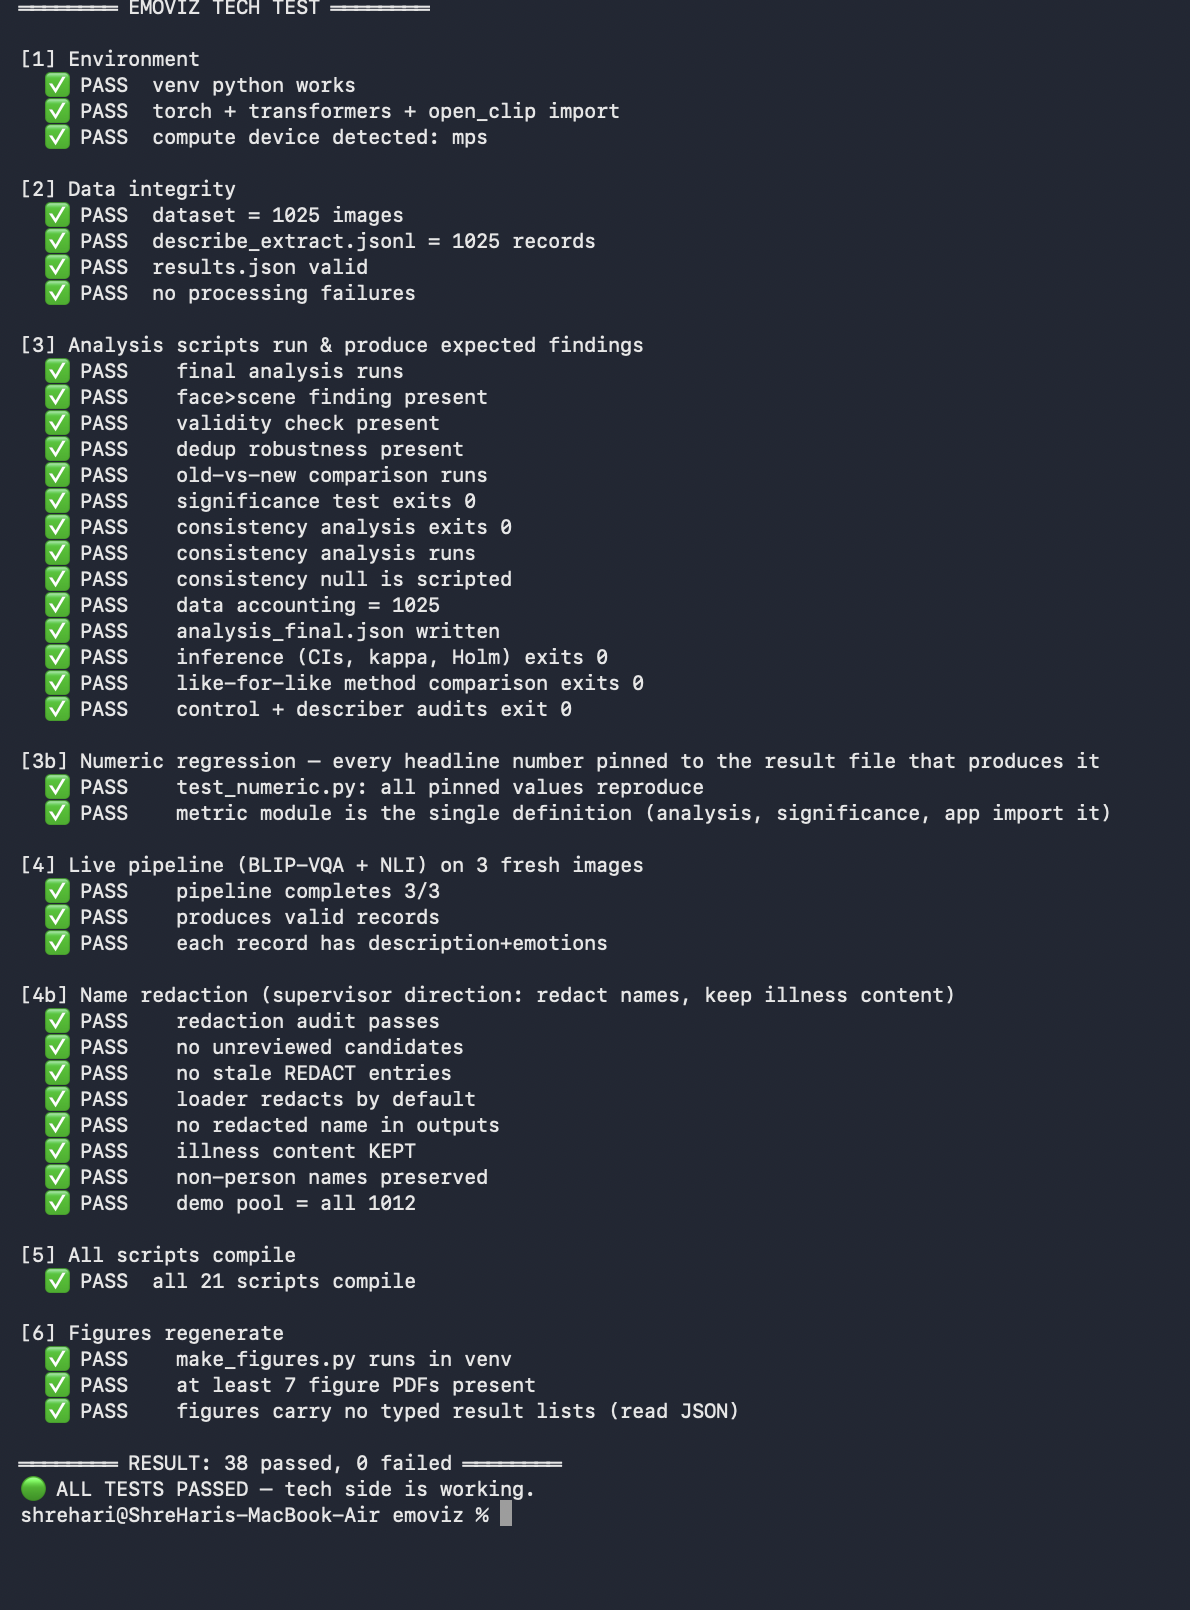
\includegraphics[width=0.82\textwidth]{test_suite}
\caption{The automated self-test after a full run (\texttt{bash emoviz/test.sh}): the environment and data checks, every analysis script run to a clean exit, the pinned numeric regression, the live pipeline over three fresh images, the redaction audit, and the figures rebuilt from the result files.}
\label{fig:testsuite}
\end{figure}

\end{sloppypar}
  % Reproducibility
\chapter{Instruments}
\label{app:instruments}

This appendix gives the fixed strings and tables the pipeline runs on, so that any number in the dissertation can be traced to the exact question, template or mapping that produced it.

\section{The five describer questions}
The describer is asked these questions in this order, and each answer is stored per record:
\begin{enumerate}\setlength{\itemsep}{1pt}
\item \emph{What is the facial expression?} (\texttt{expression})
\item \emph{What is the person doing?} (\texttt{action})
\item \emph{What is the body posture?} (\texttt{posture})
\item \emph{How many people are there?} (\texttt{people})
\item \emph{What is in the picture?} (\texttt{scene})
\end{enumerate}
None of the questions contains the word ``emotion''.

\section{The description template}
The five answers are put into one sentence:
\begin{quote}\ttfamily
A drawing of \{people\} showing \{scene\}. The person is \{action\}, \{posture\}. The facial expression is \{expression\}.
\end{quote}
The template is applied to every record, including those where \texttt{people} is ``0'' or ``none''. The ablation variants in Section~\ref{sec:results-ablation} drop one clause at a time, fix \texttt{expression} to ``unclear'', or (the people-aware variants) reduce the sentence to ``A drawing showing \{scene\}.'' wherever no person was reported.

\section{The image reader's hypothesis}
The image reader scores each family by entailment against the hypothesis
\begin{quote}\ttfamily
This scene conveys \{family\}.
\end{quote}
for the seven families in turn, and the three highest entailment scores are kept.

\section{GoEmotions categories to families}
\begin{description}\setlength{\itemsep}{1pt}
\item[joy] admiration, amusement, approval, caring, desire, excitement, gratitude, joy, love, optimism, pride, relief
\item[sadness] disappointment, embarrassment, grief, remorse, sadness
\item[anger] anger, annoyance, disapproval
\item[fear] fear, nervousness
\item[surprise] surprise, realization, confusion, curiosity
\item[disgust] disgust
\item[neutral] neutral
\end{description}
A family's score is the sum of its members' probabilities, and the seven sums are normalised to a distribution. The grouping is the one proposed by the GoEmotions authors.

\section{Family centroids on the circumplex}
\begin{center}
\begin{tabular}{lrr}
\toprule
Family & Valence & Arousal \\
\midrule
joy & $+0.80$ & $0.60$ \\
sadness & $-0.75$ & $0.30$ \\
anger & $-0.70$ & $0.80$ \\
fear & $-0.65$ & $0.75$ \\
surprise & $+0.30$ & $0.80$ \\
disgust & $-0.70$ & $0.60$ \\
neutral & $0.00$ & $0.30$ \\
\bottomrule
\end{tabular}
\end{center}
The centroids were set by hand from the usual placement of the basic emotions on the circumplex. The smallest value of Equation~\ref{eq:va} over these seven points is $0.412$ (joy against sadness).

\section{Readable expression words}
A record is face-classified when the describer reports at least one person and its expression answer contains, as a whole token, one of:
\begin{quote}
smile, smiling, happy, sad, angry, serious, surprised, surprise, calm, excited, crying, laughing, frowning, scared, shocked, worried, concentration, concentrating, grin, grinning, neutral, confused, determined, pensive, sleepy, sleeping.
\end{quote}
The people count is parsed from digits or number words (none, one, two, \ldots, several, many, crowd, group, lots). A non-empty answer that is neither is taken to mean at least one person is present.

\section{Name redaction procedure}
\begin{enumerate}\setlength{\itemsep}{1pt}
\item \textbf{Detect.} Candidates come from three detectors: a given-name gazetteer (7,944 names), mid-sentence capitalised tokens that are absent from a 236,000-word English dictionary, and naming phrases such as ``called X'' and ``my friend X''. Recall matters more than precision here because most prompts are typed in lower case.
\item \textbf{Review.} Every candidate has a recorded decision (redact or keep) with a reason, and each redaction is tied to the record it was reviewed in. The audit fails if any candidate has no decision or if a redaction entry no longer matches anything.
\item \textbf{Apply.} At load time, per record, the token is replaced by \texttt{[name]}; consecutive placeholders collapse to one. The files on disk are never changed. Words about illness, grief and places are kept.
\end{enumerate}

\section{Single-coder check: coding instructions}
The coder works from numbered contact sheets that show only the drawings and fills four columns per drawing:
\begin{description}\setlength{\itemsep}{1pt}
\item[person] y / n: is at least one person or face drawn?
\item[face] y / n: is there a face whose expression can be read? (n if there is no person)
\item[valence] $+$ / $-$ / 0: the feeling the drawing gives, positive, negative or neither
\item[family] joy / sadness / anger / fear / surprise / disgust / neutral
\end{description}
The sample is fixed by seed: 120 drawings, made up of 40 face-classified records, 40 scene-classified records with no people reported, and every record whose people answer was vague or a bare word, topped up equally from the first two strata. The prompt, the description and the model readings are not shown during coding.
  % Instruments
\chapter{Supervision record}
\label{app:supervision}

Supervision ran roughly fortnightly from June, with a written brief prepared before each meeting. The table lists the meetings and what each one changed in the project. The direction given at the end of July shaped the whole design and is described in Chapter~\ref{ch:method}.

\begin{center}
\small
\begin{tabular}{p{2.6cm}p{10.2cm}}
\toprule
Date (2026) & What was discussed and what followed \\
\midrule
18 June & First meeting. Get to know the dataset, start reading around text-to-image generation, get the School template. \\
9 July & The two strands of the project agreed: emotion from the text, and analysis of the drawings. A six-part structure for the write-up (abstract, introduction, literature review, methodology, results, discussion), and the instruction to argue from cited evidence and not from opinion. Dataset findings presented alongside: the three filename schemes, the timestamps recovered from the image files, the thirteen pre-festival records, the repeated prompts; questions raised about the original prompt sent to the generator and about names in the data. \\
31 July & The methodological direction, and the timeline for the remaining work: measure how similar the two readings are instead of scoring matches; describe the drawing first and extract the emotion from the description; split faces from scenes and emotional from non-emotional prompts; redact names and keep illness content; build in an evaluation. \\
20 August & The demonstrator shown running live. Timing of a human-rated study discussed; agreed to write up the computational results and treat the rated study as the next step. \\
4 September & Project presentation, with a live demonstration. \\
\bottomrule
\end{tabular}
\end{center}
  % Supervision record
\end{appendices}

\end{document}
